% main.tex -- Chinese edition of the main text of the article (../main.tex and ../sections/m*.tex).
% The English main text is the source of truth; this edition translates it section by section into files of
% the same names under sections/.  Mathematics, labels and the source comments are copied unchanged.  The
% Supplementary Material stays in English (../supplement.tex); it is cited as 补充材料 with its S-numbers,
% which xr-hyper reads from ../supplement.aux (prefix S-, as in the English main text).
% Compile (one latexmk at a time; the English supplement must have been compiled first so that
% ../supplement.aux exists):  latexmk -xelatex main.tex   (XeLaTeX + BibTeX; TeX Live 2025; Fandol fonts
% ship with TeX Live).
% Every quantitative statement in main.tex and sections/*.tex carries a comment  % src: <path> (<key>)
% pointing at the results file or script it comes from; paths are relative to the repository root.
\documentclass[UTF8,a4paper,11pt,fontset=fandol]{ctexart}

% The packages of the English article.  fontenc (T1), inputenc and lmodern are not loaded: under XeLaTeX the
% ctex/fontspec setup supplies Unicode (TU) Latin Modern for Latin text and Fandol for Chinese.
\usepackage[a4paper,margin=2.5cm]{geometry}
\usepackage{amsmath,amssymb,amsthm}
\usepackage{graphicx}
\usepackage{booktabs}
\usepackage{array,longtable,multirow}
\usepackage{enumitem}
\usepackage[font=small,labelfont=bf]{caption}
\usepackage{microtype}
\usepackage[numbers,sort&compress]{natbib}
\usepackage{xcolor}
\usepackage{xr-hyper}
\usepackage[colorlinks=true,linkcolor=blue!50!black,citecolor=blue!50!black,urlcolor=blue!50!black]{hyperref}
\externaldocument[S-]{../supplement}
% Links to the supplement are GoToR actions with a named destination.  Under XeLaTeX, hyperref keeps the page
% value of the first remote link and then warns `Invalid page number (0)' at every later one; the page value is not
% used when a named destination is given, so it is reset before each remote link (no \href with page= is used).
\makeatletter
\let\zh@MakeRemoteAction\Hy@MakeRemoteAction
\def\Hy@MakeRemoteAction{\let\Hy@href@page\@empty\zh@MakeRemoteAction}
\makeatother

\usepackage[section]{placeins}   % floats stay inside the section that defines them

\renewcommand{\topfraction}{0.92}
\renewcommand{\bottomfraction}{0.80}
\renewcommand{\textfraction}{0.06}
\renewcommand{\floatpagefraction}{0.75}
\setcounter{topnumber}{3}
\setcounter{bottomnumber}{2}
\setcounter{totalnumber}{4}

% Chinese typesetting: left-aligned section headings (as in the English article), caption label followed by
% a quad (图 3  ……), run-in paragraph headings.
\ctexset{
  section       = {format = \Large\bfseries\raggedright},
  subsection    = {format = \large\bfseries\raggedright},
  subsubsection = {format = \normalsize\bfseries\raggedright},
  paragraph     = {format = \bfseries, runin = true, afterskip = 0pt},
}
\captionsetup{labelsep=quad}
\pagestyle{plain}                 % page number at the foot, no running head (as in the English article)

\hypersetup{pdftitle={室内传染病流行的随机游走 SIR 模型：再生数、离散个体，以及以暴发记录、接触记录和示踪测量为对照的预先设定检验},
  pdfauthor={周易潇潇（Xiaoxiao Zhouyi）},
  pdfkeywords={室内传播；格点随机游走；基本再生数；下一代矩阵；配对层次理论；随机模拟；暴发数据；接触网络；%
  示踪测量；预先设定的检验}}

\graphicspath{{figures/}}
% macros.tex -- notation and theorem environments of the Chinese edition of the main text.
% Identical to ../macros.tex in every notation macro (all mathematics is unchanged).  Only three
% things differ: (1) the unit words of \perday, \cdunit and \cellday are Chinese (天 = day, 格 = cell),
% matching the axis labels of the *_zh figures; (2) the theorem environments carry Chinese names; (3) theorem
% bodies are upright and notes are in full-width brackets (Chinese typesetting).
% Loaded by main.tex (ctexart, XeLaTeX) after amsmath, amssymb, amsthm.  The notation is typeset as Table "appD_tables:tab:notation"
% (Supplementary Section S1); the comment table below adds, in its last column, the names used in the code.
%
% =====================================================================================================
% NOTATION TABLE (mapping to the code in the last column)
% -----------------------------------------------------------------------------------------------------
%  symbol            macro            meaning                                             code
% -----------------------------------------------------------------------------------------------------
%  \Omega            \cells           set of walkable lattice cells (barriers removed)    Omega
%  n                 \ncell           number of walkable cells, n = |\Omega|              n (theory), M or |Omega| (sim)
%  x, y, z           --               cells (elements of \Omega)                          r, s (theory); x, y (sim)
%  a                 --               lattice spacing (m); lengths in cells unless stated a
%  D_x               --               mobility (diffusion coefficient) of cell x, cell^2/day   D(r)
%  D_0               \Dz              mobility scale: D_x = D_0 d_x, d_x the zone multiplier    D0
%  \omega_{x\to y}   \hop{x}{y}       hop rate from x to a neighbouring cell y (1/day)    w_{s->r}, W(x->y)
%  \mathbf M         \gen             movement generator, M_{yx} = \omega_{x\to y}, 1^T M = 0   M (theory), L (sim)
%  \mathbf M_0       \genz            generator at D_0 = 1, so M = D_0 M_0
%  \boldsymbol\pi    \stat            stationary distribution of M (uniform for the symmetric rule)  pi
%  P_t(y|x)          --               propagator, (e^{Mt})_{yx}                           P_t(r|s), G
%  q_x, \mathbf Q    \Qm              infection efficiency of cell x; Q = diag(q)         q, Q
%  \beta, \gamma     --               transmission rate, recovery rate (1/day)
%  \mathbf P         \ker             contact kernel, row-stochastic, P_{xy} = P(y|x)     P (sim)
%  N                 \Npop            number of people in the room                        N, N_tot
%  S_x, I_x, R_x     --               expected numbers of susceptible/infective/recovered in cell x
%  \mathbf J         \Jm              growth operator J = M + F - \gamma 1                J
%  \mathbf F, \mathbf V  \Fm, \Vm     transmission and transition parts; F = \beta P^T Q (= \beta Q for the same-cell kernel), V = \gamma 1 - M
%  \mathbf K         \ngm             next-generation matrix K = F V^{-1}                 K
%  n_off(x)          \noff            offspring number: column sum of K (mean-field secondary cases of a case born at x)
%  R_0               \Rz              basic reproduction number of the mean-field model, \rho(K)
%  \lambda_1         \lamone          growth rate s(J)                                    lambda_1
%  s(A), \rho(A)     \sabs, \srad     spectral abscissa, spectral radius
%  <q>_\pi           \qmean           \sum_x \pi_x q_x  (plain <q> when \pi is uniform)   <q>_pi
%  q_max, q_min      \qmax, \qmin
%  u, \ell           \uvec, \lvec     right/left Perron vectors of J (prevalence map; u sums to 1)   u, l
%  w, z              \wvec, \zvec     right/left Perron vectors of K (incidence map; reproductive value)   w, z  (sim: v, u)
%  e_x               \evec            elasticity map, e_x = d ln R0 / d ln q_x            e
%  \mathcal E(v)     \dirich          Dirichlet form of the reversible generator          E(x)
%  \mu_k, \phi_k     --               eigenvalues/eigenvectors of -M (reversible case), \mu_0 = 0
%  Z, \mu_Z          \muZ             a set of cells (zone); exit rate \mu_Z = -s(M[Z,Z])
%  \kappa_x          --               exit (door) rate from cell x; M_\kappa = M - diag(\kappa)
%  \mu_leak          \muk             leak rate, -s(M_\kappa)
%  R_0^{room}        \Rroom           reproduction number of a leaky room
%  \bar\rho          \rhobar          mean number of OTHER people per cell, (N-1)/n       rho_bar
%  h(x,y)            --               pair hazard \beta q_x P(y|x)/\bar\rho               h
%  p(x,y)            --               probability that a case born at x infects a given person then at y
%  R_1(x)            \Rone            expected secondary cases of a lone index case born at x (pair level)
%  \bar R_1          \Ronebar         R_1 averaged over a uniformly placed index case      "pair R1", "R1 uniform index"
%  \mathbf K_1       \ngmone          pair-level next-generation matrix                   K1
%  g_0               \gz              Laplace-transformed return probability of the relative walk at \gamma
%  c_x               --               encounter factor of the per-cell rule
%  \hat R            \Rhat            counted mean number of secondary cases in simulation
%  f                 --               fraction of the day a room is occupied (duty cycle)
%  M0, M1, M2        \Mzero,\Mone,\Mtwo  validation models: well mixed; same-site; with non-local airborne term
%  \varepsilon_k     --               infectiousness parameter of outbreak event k
%  X_j               --               model exposure of susceptible j
%  D_p, D_{air}      \Dp, \Dair       calibrated mobility of people (M1) and mixing coefficient of quanta (M2), m^2/h
%  \Lambda           \remrate         removal rate of airborne quanta (ventilation + deposition + inactivation), 1/h
% -----------------------------------------------------------------------------------------------------
%  Units: time in days and lengths in lattice cells in Sections 2-6 (D in cell^2/day, a = 1);
%         hours and metres in Section 7 (D_p, D_air in m^2/h).
%  Default epidemiological parameters: \beta = 0.5/day, \gamma = 0.14/day.
% =====================================================================================================

% --- sets, vectors, matrices
\newcommand{\cells}{\Omega}
\newcommand{\ncell}{n}
\newcommand{\Npop}{N}
\newcommand{\Dz}{D_0}
\newcommand{\hop}[2]{\omega_{#1\to #2}}
\newcommand{\gen}{\mathbf{M}}
\newcommand{\genz}{\mathbf{M}_0}
\newcommand{\genk}{\mathbf{M}_{\kappa}}
\newcommand{\stat}{\boldsymbol{\pi}}
\newcommand{\Qm}{\mathbf{Q}}
\renewcommand{\ker}{\mathbf{P}}          % contact kernel (the operator \ker is not used in this article)
\newcommand{\Jm}{\mathbf{J}}
\newcommand{\Fm}{\mathbf{F}}
\newcommand{\Vm}{\mathbf{V}}
\newcommand{\ngm}{\mathbf{K}}
\newcommand{\ngmone}{\mathbf{K}_1}
\newcommand{\Id}{\mathbf{1}}             % identity matrix
\newcommand{\one}{\boldsymbol{1}}        % vector of ones
\newcommand{\uvec}{\mathbf{u}}
\newcommand{\lvec}{\boldsymbol{\ell}}
\newcommand{\wvec}{\mathbf{w}}
\newcommand{\zvec}{\mathbf{z}}
\newcommand{\evec}{\mathbf{e}}
\newcommand{\qvec}{\mathbf{q}}
\newcommand{\T}{\mathsf{T}}              % transpose
\newcommand{\diag}{\operatorname{diag}}

% --- spectral quantities and reproduction numbers
\newcommand{\sabs}{s}                    % spectral abscissa s(A)
\newcommand{\srad}{\rho}                 % spectral radius \rho(A)
\newcommand{\Rz}{R_0}
\newcommand{\Rroom}{R_0^{\mathrm{room}}}
\newcommand{\Rone}{R_1}
\newcommand{\Ronebar}{\bar{R}_1}
\newcommand{\Rhat}{\widehat{R}}
\newcommand{\lamone}{\lambda_1}
\newcommand{\qmean}{\langle q\rangle_{\pi}}
\newcommand{\qmax}{q_{\max}}
\newcommand{\qmin}{q_{\min}}
\newcommand{\muZ}{\mu_Z}
\newcommand{\muk}{\mu_{\mathrm{leak}}}   % leak rate (not \mu_\kappa: too close to \mu_k in print)
\newcommand{\noff}{n_{\mathrm{off}}}      % offspring number (column sum of K)
\newcommand{\dirich}{\mathcal{E}}
\newcommand{\rhobar}{\bar{\rho}}
\newcommand{\gz}{g_0}

% --- validation models and parameters
\newcommand{\Mzero}{\mathrm{M0}}
\newcommand{\Mone}{\mathrm{M1}}
\newcommand{\Mtwo}{\mathrm{M2}}
\newcommand{\Dp}{D_{\mathrm{p}}}
\newcommand{\Dair}{D_{\mathrm{air}}}
\newcommand{\remrate}{\Lambda}

% --- probability
\newcommand{\Prob}{\mathbb{P}}
\newcommand{\Exp}{\mathbb{E}}
\newcommand{\dd}{\mathrm{d}}
\newcommand{\e}{\mathrm{e}}

% --- units and small helpers (unit words localised for the Chinese edition; the mathematics is unchanged)
\newcommand{\perday}{\,\text{天}^{-1}}
\newcommand{\cdunit}{\ensuremath{\text{格}^2\cdot\text{天}^{-1}}}   % the unit of mobility, in text or math
\newcommand{\cellday}{\ensuremath{\,\text{格}^2\cdot\text{天}^{-1}}} % the same after a number
\newcommand{\pct}{\,\%}                                                  % per cent after a number
\newcommand{\sqmh}{\,\mathrm{m}^2\,\mathrm{h}^{-1}}
\newcommand{\qph}{\,\mathrm{quanta}\,\mathrm{h}^{-1}}

% --- theorem environments (one counter per section; numbering 定理 3.1, 命题 3.2, ...)
% One style for all environments: bold head, upright body, optional note in full-width brackets.
\newtheoremstyle{zhthm}{\topsep}{\topsep}{\normalfont}{}{\bfseries}{}{1em}%
  {\thmname{#1}\thmnumber{\ #2}\thmnote{\mdseries（#3）}}
\theoremstyle{zhthm}
\newtheorem{theorem}{定理}[section]
\newtheorem{proposition}[theorem]{命题}
\newtheorem{lemma}[theorem]{引理}
\newtheorem{corollary}[theorem]{推论}
\newtheorem{conjecture}[theorem]{猜想}
\newtheorem{definition}[theorem]{定义}
\newtheorem{assumption}{假设}
\renewcommand{\theassumption}{\Alph{assumption}}
\newtheorem{observation}[theorem]{数值观察}
\newtheorem{example}[theorem]{例}
\newtheorem{remark}[theorem]{注}

% Proof: bold head without a full stop (证明 / the optional title), upright body, QED box as in amsthm.
\makeatletter
\renewenvironment{proof}[1][\proofname]{\par
  \pushQED{\qed}%
  \normalfont \topsep6\p@\@plus6\p@\relax
  \trivlist
  \item[\hskip\labelsep\bfseries #1\quad]\ignorespaces
}{%
  \popQED\endtrivlist\@endpefalse
}
\makeatother
\renewcommand{\proofname}{证明}

% Generated table bodies (data/v2_tab_*.tex, written by code/v2_numbers.py) are read with the primitive \input,
% which is expandable, so that a rule may follow the last row.
\makeatletter
\newcommand{\tabinput}[1]{\@@input #1.tex }
\makeatother


% State of the repository named in the availability statement.  make_release.py tests the URL and the
% version tag when the release is built and writes repo_status.tex (\repopublictrue, \repotaggedtrue as
% found).  This edition reads its own repo_status.tex if a build writes one, and otherwise that of the English
% edition (../repo_status.tex); without either file the cautious wording is used.
\newcommand{\repoversion}{1.2.0}
\newif\ifrepopublic
\repopublicfalse
\newif\ifrepotagged
\repotaggedfalse
\InputIfFileExists{repo_status.tex}{}{\InputIfFileExists{../repo_status.tex}{}{}}

\title{室内传染病流行的随机游走 SIR 模型：\\再生数、离散个体，以及以暴发记录、\\
接触记录和示踪测量为对照的预先设定检验%
\thanks{本文为英文论文正文的中文版。补充材料为英文，文中以“补充材料”及其带前缀 S 的编号引用。}}

\author{周易潇潇（Xiaoxiao Zhouyi）\\[4pt]
\normalsize 英国布里斯托大学工程数学与技术学院\\
\normalsize \href{mailto:zhouyixiaoxiao@gmail.com}{zhouyixiaoxiao@gmail.com}}

\date{\vspace{-1.5ex}2026\vspace{-2ex}}

\begin{document}
\maketitle

\begin{abstract}
本文研究格点上独立随机游走者之间的 SIR 流行，其中迁移率与传染效率随格点而异。
(i)~平均场 $\Rz$ 是由格点传播子构成的下一代矩阵的谱半径。对同格传播，其上下界、极限以及随迁移率的单调递减均成立，
这些结论对斑块模型而言已为人所知；对其他接触核，下界与单调性可能不成立。在传染效率均匀时，封闭房间的 $\Rz$ 与其尺寸、
形状和迁移率无关；在所述条件下，泄漏将 $\gamma$ 替换为 $\gamma+\muk$。
(ii)~双游走者理论给出单独传播的指示病例所致第一代病例数的精确均值；在低占据率和低迁移率下，它低于 $\Rz$
（办公室场景中为 2.27，而 $\Rz$ 为 5.11），且不是阈值量。
% src: data/s5_pair_large_sample.json (office|D0=1: R1bar_exact 2.2661, counted 2.265 +- 0.004 in 400,000 runs, R0_ngm 5.1073; office|D0=100: R1bar_exact 4.3411, R0_ngm 4.646)
(iii)~在四个封闭房间场景的精确模拟中，空间效应仅在极低迁移率下才较大。
(iv)~五项检验（其方案均在受检模型运行之前确定；方案撰写时已知晓数据，其时间先后为自证，且未经登记）将模型与 38 条暴发记录中的 22 条、
接触记录、示踪测量以及一次学校疫情相对照。模型与这些数据之间不存在普遍一致。同格点传播未得到支持；游走产生的接触在
全部六个接触数据集上均未通过。空气传播扩展模型对留出事件距离梯度的预测优于均匀混合模型（对数得分增益 $+14.35$；
若暴发服从恒定的近/远比值，该模型也会以 0.65--0.73 的概率做到这一点），但预先设定的合并比较支持恒定比值（$-9.15$，其中十分之九来自
单个事件，而该事件的近区是根据其自身数据选定的）；在四个留出航班上，两者不分高下。罹患率是拟合得到的；随格点而异的迁移率仍未
得到检验。
% src: data/bsc_outbreaks/outbreaks.csv (27 rows); code/bsc_validation2/a1_more_outbreaks/PREREGISTRATION.md section 2.1 (11 records); 22 records in a test: 2 + 5 (first), 6 + 5 (second), and T3, C3, S1, T7 in the level checks and negative controls of the first test (outbreaks.csv protocol_role); data/v2_numbers.json (con.ladder: A0 on all six datasets); data/v2_numbers.json (out2.pooled.M2.all: delta0 14.351, deltaC -9.150; out2.pooled.plant_share_of_deltaC 0.916; out2.pooled.M2.air: deltaC -0.77; out2.power.registered: CRR P_B1 0.652; out2.power.corrected: CRR B1 0.732); notes/VERIFICATION.md section 4.10 (statement and reservations)
% src: data/s2_model_scenes.json (scenes.<name>.R0_1m: excess over the well-mixed value below 0.03 % at walking mobility)
\end{abstract}

\noindent\textbf{关键词：}室内传播；格点随机游走；基本再生数；下一代矩阵；配对层次理论；随机模拟；暴发数据；
接触网络；示踪测量；预先设定的检验

\section{引言}\label{s1_intro:sec}
% Main text, Section 1 (Introduction).
% Paths in "% src:" comments are relative to the repository root.

有记录的 SARS-CoV-2 聚集性感染绝大多数发生在室内\citep{qian2021indoor,leclerc2020settings}；在若干记录详尽的事件中，
病例在房间内的分布并不均匀：它们集中在呼叫中心楼层的一侧\citep{park2020}，在客机客舱\citep{khanh2020}或高铁
\citep{hu2021}上靠近指示病例，或位于同一台空调气流所及的相邻餐桌\citep{lu2020,li2021}。
室内风险的标准定量工具是 Wells--Riley 方程\citep{wells1955airborne,riley1978,szeto2010review}。该方程及以其为基础的
模型\citep{noakes2006modelling,bazant2021guideline}都把室内空气视为均匀混合，因而室内每个易感者承担相同的风险。
本文考察一个最简的空间模型能为这一图景增添什么：在由地面格点构成的格子上做独立随机游走的人群中的
易感–感染–恢复（SIR）流行，其中迁移率 $D_x$ 与传染效率 $q_x$ 随格点而异（工位、走廊、会议室、障碍物）。

\paragraph{已有工作。}
对移动个体中的流行病建模已有三十多年的历史：个体在格点之间移动的格点自动机\citep{boccara1992automata,rhodes1996persistence}，
在连续空间中移动的主体\citep{gonzalez2004scaling,frasca2006dynamical,buscarino2008disease}，以及集合种群网络上的
反应–扩散过程\citep{colizza2007reaction,belik2011natural,wang2014spatial}。
与本文模型最接近的是两个游走者之间传播的随机游走理论：当一个感染游走者与一个易感游走者相遇时，感染作为一种
以有限速率发生的反应而出现\citep{kenkre2014theory,sugaya2018analysis,kenkre2021theory}。\citet{giuggioli2022spatio}
借助精确传播子\citep{giuggioli2020exact,sarvaharman2023particle}在格点上表述了这一理论，并对移动的易感者、感染者和
恢复者解析地预测了基本再生数。
多游走者系统本身是概率论与统计物理中的经典研究对象。对于 $\mathbb{Z}^d$ 上独立的连续时间随机游走者（感染者与
健康者相遇时发生感染），\citet{kesten2005spread,kesten2008shape} 证明了感染集合随时间线性增长并具有渐近形状；
在感染游走者会恢复且可再次被感染的情形下，他们还证明了存在一个临界恢复率：低于该值时感染以正概率存续，高于该值时
感染消亡\citep{kesten2006phase}。同一过程在物理学中称为扩散流行过程（diffusive epidemic process），其吸收态相变已
通过平均场理论与模拟进行了分析\citep{maia2007diffusive}；在本文这样的永久免疫情形下，正方格子上的模拟显示出一个由
游走者密度控制的动态渗流型相变\citep{carvalho2025generalized}。这些结果针对的是无限的或大型的均匀格子。它们确立了
游走者系统中阈值的存在，但没有给出本文所考虑的小型异质房间中阈值的取值。
% src: data/refs_search.json (kesten2005spread, kesten2006phase, kesten2008shape, maia2007diffusive, carvalho2025generalized: Crossref records, abstracts in manual_checks; search queries of 1 October 2026)

对仓室模型，基本再生数 $\Rz$ 是下一代算子的谱半径\citep{diekmann1990definition}，即 $\Rz=\srad(\Fm\Vm^{-1})$，并且它是
一个阈值\citep{vandendriessche2002reproduction}。在无病平衡态处线性化后，格点模型的平均场版本就是一个采用标准发生率的
传染病斑块模型，相关定理均已发表。
对移动对称的斑块模型，\citet{allen2007asymptotic} 定义了 $\Rz=\srad(\Fm\Vm^{-1})$，证明了阈值性质，证明了增长界
$\sabs(\Fm-\Vm)$ 随扩散速率在其两个极限之间递减，并猜想 $\Rz$ 具有同样的单调性；该猜想由\citet{gao2019travel} 对对称
移动情形、由\citet{gao2020fast} 对一般情形给出证明（另见\citet{chen2020asymptotic}），它是\citet{altenberg2012resolvent}
的约化原理的一个实例。$\Rz$ 介于最小与最大的斑块再生数之间、且在二者相等时与移动无关，这一结论来自\citet{gao2011sis}；
更紧的下界（即快速扩散极限）来自\citet{gao2020fast}；以扩散速率倒数的一阶趋近该极限的结果由\citet{tien2015disease}
得到，其研究对象是一个由病原体而非宿主移动的网络，下一代矩阵具有相同的形式。连续情形的对应结果见
\citet{allen2008asymptotic} 与\citet{wang2012basic}。（我们阅读了\citet{gao2011sis} 与\citet{tien2015disease} 的正式发表
版本，其 Proposition~2.2 与第 4.2 节包含了我们归于它们的结果；也阅读了\citet{gao2020fast} 的正式发表版本。
对\citet{allen2007asymptotic} 与\citet{gao2019travel}，我们只阅读了摘要；我们归于它们的结论依据\citet{gao2020fast}
的转述，并在摘要所及的范围内与摘要一致：前者为阈值性质，后者为对称移动情形下随扩散速率的单调递减。）
% src: data/refs_search.json (gao2020fast_published: Theorems 2.1, 2.3, 3.3, Corollary 3.5 "generalization of Lemma 3.4 in Allen et al.", Discussion on Tien et al.; checked 1 October 2026)
% src: published versions of doi:10.1016/j.mbs.2011.05.001 (Proposition 2.2: max{max_i tilde R0^(i), min_i R0^(i)} <= R0 <= max_i R0^(i)) and doi:10.1007/s00285-014-0791-x (Section 4.2, eqs. (29)-(35): first-order Laurent correction of R0 in 1/d_W with the generalised group inverse X_0), author copies read 2 October 2026
% src: abstracts of doi:10.1137/060672522 and doi:10.1137/18M1211957 in their Crossref records (read 2 October 2026)

空间分辨的室内模型也已存在：分区通风模型\citep{noakes2009mathematical}，空气中浓度的输运模型
\citep{lau2022predicting,vuorinen2020modelling}，以及针对超市和航空旅行的基于行人或基于主体的模拟
\citep{ying2021modelling,namilae2017multiscale}。它们对空气或运动轨迹的刻画比格点游走更为细致。与之相比，格点模型
能提供的是对再生数的解析处理；而正如第~\ref{s8_outbreaks:sec}~节所示，它所欠缺的是对共享空气的就座人群以及
“谁与谁相遇”的恰当描述。

有三类测量与这样的模型相关，每一类都有各自的文献。室内人与人之间的近距离接触已在学校、办公室、医院和会议中用
可穿戴传感器记录下来；这些接触集中于少数反复出现的接触对象，按群组组织，且时长分布很宽
\citep{cattuto2010dynamics,stehle2011high,genois2015data,genois2018can}；在有吸引力的个体附近减速的平面随机游走者
能再现其中若干统计特征\citep{starnini2013modeling}；人们也已在实测网络上模拟了流行
\citep{stehle2011simulation,gemmetto2014mitigation}。交通工具中气溶胶的输运已用示踪测量过
\citep{kinahan2021aerosol,woodward2022evaluation,ou2022}，房间的湍流扩散系数也已与其通风联系起来
\citep{cheng2011modeling}。此外，暴发调查按距离报告风险：航空器上的接触追踪采用病例周围两排的范围，这一规则的局限
是已知的\citep{hertzberg2016risk}；学校中的流感传播也已被分解到班级、年级与学校层面\citep{endo2021within}。
第~\ref{s8_outbreaks:sec}~节正是以这些数据检验模型；这些数据所提示的规则——恒定的近/远风险比与固定的组内接触
份额——就是模型必须胜过的通用竞争模型。

\paragraph{本文贡献。}
\begin{enumerate}[label=(\roman*),leftmargin=2.2em,itemsep=1pt,topsep=3pt]
\item \emph{平均场再生数}（第~\ref{s3_r0:sec}~节和第~\ref{s4_geometry:sec}~节）。我们叙述并证明
  $\Rz=\srad\bigl(\beta\Qm(\gamma\Id-\gen)^{-1}\bigr)$，即由经拉普拉斯变换的格点传播子构成的下一代矩阵的谱半径。对同格
  传播，我们证明 $\beta\qmean/\gamma\le\Rz\le\beta\qmax/\gamma$，证明 $\Rz$ 随迁移率尺度在这两个极限之间单调递减，并证明
  任一高风险分区都给出一个下界；对其他接触核，下界与单调性都可能不成立。在 $q$ 均匀的封闭房间中，$\Rz$ 与房间的
  尺寸和形状无关。真正的边界效应是泄漏（门、有限的停留时间）：对均匀 $q$ 与同格接触核，或对不依赖于位置的停留时间
  与任意接触核，泄漏将 $\gamma$ 替换为 $\gamma+\muk$；对异质 $q$ 与同格接触核，它给出
  $\beta\langle q\rangle_\nu/(\gamma+\muk)\le\Rroom\le\beta\qmax/(\gamma+\muk)$
  （定理~\ref{s4_geometry:thm:leaky}）；当采用其他接触核且门为局部时，该公式与两个界都可能不成立。
\item \emph{离散个体}（第~\ref{s5_pair:sec}~节）。沿用双游走者传播理论\citep{kenkre2014theory,giuggioli2022spatio}，
  把感染处理为双游走者过程中的一个部分吸收缺陷。由此得到一个指示病例所致二代病例数的期望 $\Rone(x)$，以及均匀周期
  房间与无限大地面情形下的闭式解；在所检验的情形中，该闭式解对反射壁房间的近似误差在 1\,\% 以内。它解释了为何在
  低占据率下计数得到的二代病例数低于 $\Rz$，以及对离散的人而言有限尺寸效应取何种形式。
  % src: data/s5_pair_checks.json (finite_size: largest deviation of the closed form from the exact pair solve 0.90 %, 21 rooms)
\item \emph{精确随机模拟}（第~\ref{s6_scenes:sec}~节）：模拟四个场景（办公室、超市、教室、地铁车厢）与干预措施，
  其中二代病例数由感染树计数得到，而非拟合得到。
\item \emph{与数据对照}（第~\ref{s8_outbreaks:sec}~节）。我们汇集了 38 条有文献记录的室内暴发与暴露队列记录：
  第一数据集包含来自 31 篇已发表文献的 27 条记录（其中 23 条有病例数与暴露人数），第二数据集包含十起暴发的十一条
  带座位或位置数据的记录。在其中 18 条记录上，两项样本外检验把两个空间模型（$\Mone$、$\Mtwo$）与均匀混合模型
  （$\Mzero$）相比较（第一项用两条记录标定、五条留出；第二项为六条与五条；另有四条记录进入第一项检验的水平检验与
  阴性对照）；第二项检验按设计还把它们与恒定的近/远风险比相比较。另有三项分析处理暴发计数无法回答的问题：把格点
  游走产生的接触与六个室内场所的实测接触相比较；由已发表的示踪测量确定空气传播核，再与暴发数据对照；把模型约化到
  分区层面，以一所学校中测得的混合为输入，预测另外 29 所学校中的一次流感疫情。五项主要检验中的每一项，都遵循一份
  在受检模型于其数据上运行之前写成的方案（对示踪分析而言，所用暴发在其他模型下的结局已知）。这些方案是预先设定的，
  而不是通常意义上的预注册：撰写时数据已知，未提交任何登记平台，其时间先后仅以文件哈希值与文件时间戳为凭。在结果
  已知之后添加的比较均标为事后比较；全部检验的登记表注明了哪些是事先设定的（补充材料表~\ref{S-appS_prot2:tab:register}）。
  所有结果均连同其失败之处一并报告。
  % src: data/bsc_outbreaks/outbreaks.csv (27 rows); code/bsc_validation2/a1_more_outbreaks/PREREGISTRATION.md section 2.1; notes/VERIFICATION.md (Section 4.4, outbreak dataset); notes/VERIFICATION.md (Section 4.5, first outbreak test: pre-registration data-aware, model-blind); notes/VERIFICATION.md section 4.10 (reservations)
\end{enumerate}

\paragraph{已知结果与本文新增内容。}
表~\ref{s1_intro:tab:known} 将二者区分开来。关于平均场 $\Rz$ 的定理对斑块模型是已知的。我们仍从非负矩阵的标准结论
出发给出完整证明（补充材料第~\ref{S-appS_r0:sec}~节），原因在于条件至关重要：下界 $\beta\qmean/\gamma\le\Rz$ 对同格
接触核成立，对一般接触核则不成立，对此我们给出一个三格点反例（命题~\ref{s3_r0:prop:kernel}）。
% src: data/plan_theory_checks.json (checks: kernel_counterexample, 0.50 against mean q 0.667)
双游走者形式体系属于已有工作，它所刻画的相邻个体之间接触的饱和也是一个经典效应
\citep{ball1997epidemics,keeling1999effects,durrett1994importance}。特别地，\citet{giuggioli2022spatio} 已经由双游走者
形式体系推导出封闭区域中一个感染游走者在均匀分布的易感游走者中造成的平均二代感染数，并与模拟进行了核对；单缺陷
解来自\citet{szabo1984localized}。本文新增的内容范围更窄（第~\ref{s5_pair:sec}~节）：按占据率对配对风险率进行归一化，
使配对层次的再生数与平均场再生数指向同一个模型，并给出逐元素比较 $\ngmone\le\ngm$；含接触核的异质房间中的
$\Rone(x)$ 与矩阵 $\ngmone$；周期房间与无限大地面的闭式解及其极限；与第二代的比较；以及 $\Ronebar$ 与 $\ngmone$ 的
谱半径都不是阈值量这一观察（注~\ref{s5_pair:rem:threshold}）。上述关于新增内容的陈述基于一次定向检索（2026 年
10 月 1 日在 Crossref 和 arXiv 上就随机游走者之间的感染、扩散流行过程和斑块模型再生数进行的查询），而非系统综述。
% src: data/refs_search.json (searches: queries and numbers of records screened)

\begin{table}[tbp]
\centering\small
\caption{本文结果、其已知出处与本文新增内容。表中“Thm”编号指 \citet{gao2020fast} 正式发表版本中的定理编号。
第 1--6 行与第~8 行不主张新颖性；第 9 行与第~10 行中的数据来自所引文献，新增的是这些数据的汇编与数字化以及检验。}
\label{s1_intro:tab:known}
\begin{tabular}{@{}>{\raggedright\arraybackslash}p{0.27\textwidth}>{\raggedright\arraybackslash}p{0.31\textwidth}>{\raggedright\arraybackslash}p{0.35\textwidth}@{}}
\toprule
结果 & 已知出处 & 本文新增 \\
\midrule
1.\ $\Rz=\srad(\Fm\Vm^{-1})$ 及其阈值性质 &
  \citep{diekmann1990definition,vandendriessche2002reproduction}；斑块模型见
  \citep{allen2007asymptotic} &
  用格点记号给出的证明；模态公式，其最大的对角项是一个下界 \\\addlinespace[2pt]
2.\ $\beta\qmean/\gamma\le\Rz\le\beta\qmax/\gamma$ &
  介于最小与最大的斑块再生数之间\citep{gao2011sis}；下界\citep{gao2020fast} Thm~3.3；
  连续情形\citep{allen2008asymptotic}；异质性提高 $\Rz$ \citep{hasibeder1988population} &
  成立条件（同格接触核）以及对其他接触核的反例 \\\addlinespace[2pt]
3.\ $\Rz$ 随迁移率递减，介于第~2 行的两个极限之间 &
  \citep{allen2007asymptotic}中提出猜想；\citep{gao2019travel}（对称移动）与
  \citep{gao2020fast} Thm~2.3（一般情形）给出证明；\citep{chen2020asymptotic,altenberg2012resolvent} &
  四个室内场景中该效应的大小，分别在低迁移率与现实迁移率下 \\\addlinespace[2pt]
4.\ 均匀 $q$：无论移动方式如何，$\Rz=\beta q/\gamma$ &
  \citep{gao2011sis}；经吸收边界的损失\citep{skellam1951random,cantrell2003spatial} &
  对房间的推论（封闭时无尺寸效应）；泄漏房间公式 $\Rroom=\beta q/(\gamma+\muk)$
  （同格接触核） \\\addlinespace[2pt]
5.\ 分区下界；快混合与慢混合的渐近展开；逐边单调性 &
  快速扩散展开\citep{tien2015disease}；其余为同一矩阵理论的初等推论，定向检索未找到其出处 &
  针对室内格子的陈述与证明 \\\addlinespace[2pt]
6.\ 热点分布图（Perron 向量、弹性） &
  标准的特征向量敏感性分析 &
  在各场景上的应用；关于暂态的一项提醒 \\\addlinespace[2pt]
7.\ 感染作为两个游走者之间的反应；一个感染游走者造成的平均二代感染数 &
  \citep{kenkre2014theory,sugaya2018analysis,giuggioli2022spatio,kenkre2021theory}；单缺陷
  \citep{szabo1984localized}；局部饱和
  \citep{ball1997epidemics,keeling1999effects,durrett1994importance}；无限格子上游走者的阈值
  \citep{kesten2006phase,maia2007diffusive,carvalho2025generalized} &
  按占据率归一化的风险率与 $\ngmone\le\ngm$；含接触核的异质房间中的 $\Rone(x)$ 与 $\ngmone$；周期房间与
  无限大地面的闭式解；第二代；不是阈值
  \\\addlinespace[2pt]
8.\ 扩散气溶胶暴露项；风险随距离下降 &
  \citep{lau2022predicting,venkatram2021modeling,cheng2011modeling}；航空器上的两排规则
  \citep{hertzberg2016risk} &
  仅作为第~\ref{s8_outbreaks:sec}~节中受检的扩展使用；不主张其预测优于恒定比值 \\\addlinespace[2pt]
9.\ 暴发调查 &
  补充材料第~\ref{S-appB_dataset:sec}~节中的已发表文献；此前一份以均匀混合模型评估的暴发汇编
  \citep{peng2022practical} &
  38 条记录：第一数据集中八条记录的近/远分层、呼叫中心的座位图、高铁队列的座位偏移矩阵，以及第二数据集中
  十一条带座位或位置数据的记录；两项预先设定的样本外检验及其结局 \\\addlinespace[2pt]
10.\ 实测接触、示踪测量、学校疫情的班级结构 &
  \citep{cattuto2010dynamics,stehle2011high,genois2018can,kinahan2021aerosol,woodward2022evaluation,endo2021within}；
  在他人附近减速的游走者\citep{starnini2013modeling} &
  以这些数据对游走产生的接触、采用实测系数的接触核以及分区层面约化进行的预先设定检验，结局为否定性的或弱的 \\
\bottomrule
\end{tabular}
\end{table}

\paragraph{主要发现。}
在办公室场景中（234 个可行走格点，$\beta=0.5\perday$，$\gamma=0.14\perday$，迁移率尺度 $\Dz=1\cellday$），平均场
再生数为 $\Rz=5.11$，位于界 4.64--5.36 之内；该界对分区比例相同的任何布局都成立。
% src: data/plan_theory_checks.json (office: D0=1.R0 = 5.107; lower_bound 4.643, upper_bound 5.357)
然而，当房间中有 100 个离散的人时，单个指示病例平均感染另外 $\Ronebar=2.27$ 人（配对层次的精确期望；计数值
$\Rhat=2.265\pm0.004$，为 400{,}000 次模拟的均值 $\pm$ 标准误）。
% src: data/s5_pair_large_sample.json (office|D0=1: R1bar_exact 2.2661; mean 2.2648, se 0.0039, n_runs 400000)
一半的传入感染最终消亡：暴发达到房间人数 10\,\% 的概率为 0.50，而平均场分支过程给出的是 0.78。
% src: data/bsc_sim/03_scenes.csv (office|D0=1|range1m: p_major 0.496 [0.474, 0.518], p_major_branching 0.781)
这两个数对迁移率的响应方向相反：在 $\Dz=10$ 与 $100\cellday$ 时，$\Rz$ 降至 4.68 与 4.65，而配对层次的再生数升至
$\Ronebar=3.79$ 与 $4.34$。
% src: data/s5_pair_large_sample.json (office|D0=10: R0_ngm 4.676, R1bar_exact 3.7934; office|D0=100: R0_ngm 4.646, R1bar_exact 4.3411)
在低迁移率和低占据率下，障碍物、分区隔离和容量限制会减少模拟中的暴发。其原因在于个体的离散性（一个感染者对每个
邻居只能感染一次，且反复遇到的是同一些人），而不是 $\Rz$ 更低：在频率依赖传播下，容量限制不改变 $\Rz$；分区隔离
使其升高；在 $q$ 均匀的房间中，障碍格不改变它（定理~\ref{s4_geometry:thm:closed}）；格点之间的隔断墙不能使其降低
（定理~\ref{s3_r0:thm:edges}）。
% src: data/s7_interventions_barriers.json (D=1 paired rhoB=0.10|FD attack -0.040 +- 0.003); data/bsc_sim/05_heterogeneity.json (attack_all 0.347 -> 0.231, R0_ngm 4.286 -> 4.972); data/bsc_sim/07_occupancy.json
这些效应属于一个狭窄的物理区间。格点边长为 1.5\,m 时，$\Dz=1\cellday$ 对应一天内约 3\,m 的均方根位移；5\,\% 的
时间在步行或全部时间都在步行的人对应 $2.4\times10^{3}$ 至 $4.9\times10^{4}\cellday$，在这样的迁移率下，封闭办公室的
$\Rz$ 超出其均匀混合值 $\beta\langle q\rangle/\gamma=4.64$ 不到 0.003\,\%。
% src: data/plan_theory_checks.json (office.mobility_table: D0 = 2400: +0.0027 %; D0 = 48700: +0.0001 %); data/bsc_theory/worked_examples.json (E9_physical_D: 2433.6 and 48672 cell^2/day)
驻留时间同样重要：若办公室每天占用 8 小时而非 24 小时，则一个指示病例平均感染的人数在 $\Dz=1$ 时为 0.89 至 0.93，
在 $\Dz=10\cellday$ 时为 1.34 至 1.40。
% src: data/s7_interventions_schedule.json (duty_exact|office|D0=1: exact_uniform_phase 0.8892, exact_start 0.9296; duty_exact|office|D0=10: 1.3359, 1.3975)

与数据对照时，模型并不显示普遍一致，而它所得到的正确结论也并非其所特有（第~\ref{s8_outbreaks:sec}~节）。仅在位于
同一格点的人之间传播的表述未得到支持。带扩散气溶胶项的扩展模型对风险随距离下降的预测优于均匀混合模型，但不优于
恒定的近/远风险比；它在若干事件上未通过，且不存在共同的混合系数；对第一数据集拟合得到的系数远低于在交通工具中
用示踪测得的系数。以一所学校中测得的混合份额预测另外 29 所学校中的一次流感疫情，效果仅与只含一个拟合比值的
通用模型相当。数据支持风险随距离平滑下降以及由群组主导的分区结构——这些结论是该模型与更简单的模型所共有的；
罹患率水平是拟合得到的，而非预测的；并且由于在每一起公开了人员位置的暴发中人们都是就座的或处于固定岗位，迁移率
的空间异质性仍未得到检验。我们将数据集与检验作为本文的贡献呈现，不主张模型与数据一致。
% src: notes/VERIFICATION.md (Section 4.5, first outbreak test, summary); notes/VERIFICATION.md (Section 4.10); notes/VERIFICATION.md section 4.10 (statement)

\paragraph{结果的核对方式。}
本工作的每一部分（理论、模拟、暴发数据集、两项暴发检验，以及对接触记录、示踪测量和分区结构的分析）都在同一项目内、
同一台计算机上用另行编写的代码进行了复核：第二遍重新推导了证明，重新实现了计算（包括第二个精确模拟器），根据原始
文献重新录入了暴发计数，并搜索了反例。复核并非由独立于本项目的任何人完成，也不是外部评审；在重新运行分析、比较
接触核或添加比较之处，它沿用了各项分析的数据读取程序、事件几何、转录的座位图，以及（用于计时基准测试和作息安排的）
分析所用的模拟器（补充材料第~\ref{S-appA_numerics:sec:scope}~节）。下文中，“复核”指这第二遍工作，“第二模拟器”指
其模拟器。凡复核更正了某一结果之处，报告的均为更正后的结果；复核未重新计算的结果，以及复核在结果已知之后添加的
比较，均已注明。各项复核的覆盖范围见补充材料第~\ref{S-appA_numerics:sec}~节。
% src: notes/VERIFICATION.md (Section 4.1, theory, Section 4.2, simulations); notes/VERIFICATION.md (Section 4.4, outbreak dataset); notes/VERIFICATION.md (Section 4.5, first outbreak test); notes/VERIFICATION.md (Section 4.6, second outbreak test, Section 4.7, contact records, Section 4.8, tracer measurements, Section 4.9, zone level)

\paragraph{全文结构。}
第~\ref{s2_model:sec}~节定义模型、四个场景与参数区间。第~\ref{s3_r0:sec}~节讨论平均场模型的基本再生数，
第~\ref{s4_geometry:sec}~节讨论房间尺寸、泄漏与热点分布图。第~\ref{s5_pair:sec}~节建立离散个体的配对层次理论，
第~\ref{s6_scenes:sec}~节报告场景与干预措施的模拟结果。第~\ref{s8_outbreaks:sec}~节将模型与有文献记录的暴发、实测
接触、示踪测量以及一次学校疫情相对照，第~\ref{s9_discussion:sec}~节讨论成立的结论与局限。补充材料收录证明、数值验证、
暴发数据集、检验方案、扩展表格以及全部检验的登记表；其节、公式、图和表均以前缀 S 编号。

% m2_model.tex -- Main text, Section 2: Model, scenes and parameter regime.
% Paths in "% src:" comments are relative to the repository root.
% Numbers of the two tables and of Section 2.6: code/s2_model_scene_table.py ->
% data/s2_model_scenes.json (cross-checked there against data/plan_theory_checks.json
% to 2e-13) and data/s2_model_table_rows.tex (table rows as generated).
\section{模型、场景与参数区间}\label{s2_model:sec}

本节确定模型：一条移动规则；一个带接触核的平均场模型；一个基于个体的模型（前述平均场模型即为其平均场近似）；以及三种
必须加以区分的再生数。随后描述四个场景，并说明参数所处的物理区间。在第~\ref{s2_model:sec}--\ref{s6_scenes:sec}~节
中，长度以格点为单位，时间以天为单位。

\subsection{格点上的移动}\label{s2_model:sec:movement}

房间地面由格点间距为 $a$ 的正方格子覆盖。被墙壁、家具或其他障碍物占据的格点被移除；其余 $\ncell$ 个可行走格点
构成集合 $\cells$，两个可行走格点若有一条公共边，则称二者相邻。格点 $x$ 具有迁移率（扩散系数）$D_x=\Dz d_x>0$，
其中 $\Dz$ 为迁移率尺度，$d_x$ 为无量纲的分区倍数。位于格点 $x$ 的人以如下速率跳到相邻格点 $y$：
\begin{equation}\label{s2_model:eq:hop}
  \hop{x}{y}=\hop{y}{x}=\frac{2D_xD_y}{D_x+D_y}\qquad\text{对相邻格点 } x,y\in\cells ,
\end{equation}
即两个迁移率的调和平均。这正是复合介质中扩散的有限体积离散所用的界面系数\citep{patankar1980numerical}：两个格点
之间的净流量等于 $\hop{x}{y}$ 乘以二者占据数之差，因此式~\eqref{s2_model:eq:hop} 是带反射壁的 Fick 扩散
$\partial_t\rho=\nabla\!\cdot(D\nabla\rho)$ 的一种离散。移动生成元是 $\ncell\times\ncell$ 矩阵
\begin{equation}\label{s2_model:eq:generator}
  M_{yx}=\hop{x}{y}\ (y\neq x),\qquad M_{xx}=-\sum_{y\neq x}\hop{x}{y},\qquad \one^{\T}\gen=0 ,
\end{equation}
若 $x\ne y$ 不相邻，则 $M_{yx}=0$。列指标表示出发格点：期望占据数向量满足 $\dot N=\gen N$，而 $\one^{\T}\gen=0$
表示没有人穿过墙壁进入或离开。由于 $D_x=\Dz d_x$，有 $\gen=\Dz\genz$，其中 $\genz$ 为 $\Dz=1$ 时的生成元。传播子
$P_t(y\,|\,x)=\bigl(\e^{\gen t}\bigr)_{yx}$ 是从格点 $x$ 出发的游走者在时刻 $t$ 位于格点 $y$ 的概率。对均匀矩形
格子，传播子的闭式表达已为人知\citep{giuggioli2020exact}；对本文的异质场景，所有量均由 $\gen$ 数值计算得到。

\begin{assumption}\label{s2_model:ass:A}
  可行走区域连通，即 $\gen$ 不可约。人群处于移动平衡：$N_x(t)\equiv N^*_x=\Npop\,\pi_x$，其中 $\stat>0$ 为
  $\gen$ 的平稳分布（$\gen\stat=0$，$\one^{\T}\stat=1$；在对称规则~\eqref{s2_model:eq:hop} 下，$\pi_x=1/\ncell$）。
\end{assumption}

在规则~\eqref{s2_model:eq:hop} 下矩阵 $\gen$ 对称，因此均匀分布是平稳分布，人不会在慢速分区中聚集。假设中之所以
采用一般的 $\stat$ 来表述，是因为第~\ref{s3_r0:sec}~节的若干结果对任意不可约生成元都成立。采用调和平均是一种建模
选择。速率只依赖于出发格点的规则 $\hop{x}{y}=D_x$ 是另一个模型：它关于 $\pi_x\propto1/D_x$ 满足细致平衡，因而人会
在移动缓慢之处聚集，其连续极限为 $\partial_t\rho=\nabla^2(D\rho)$。长度以格点为单位时，$D_x$ 的单位为 \cdunit{}；
以物理单位表示时，速率~\eqref{s2_model:eq:hop} 为 $2D_xD_y/((D_x+D_y)a^2)$。

\subsection{平均场模型}\label{s2_model:sec:meanfield}

位于格点 $x$ 的感染者以速率 $\beta q_x$ 产生传染性接触，其中 $\beta$ 为传染率，$q_x\ge0$ 为该格点的无量纲传染
效率（$\Qm=\diag q$，$q\not\equiv0$）。一次接触以概率 $P_{xy}=P(y\,|\,x)$ 落在格点 $y$，其中接触核 $\ker$ 为
行随机矩阵；该接触落到当时身处 $y$ 的人中均匀选取的一人身上（频率依赖发生率）。感染者以速率 $\gamma$ 恢复。
记 $S_y,I_y,R_y$ 为格点 $y$ 中易感者、感染者和恢复者的期望人数，则
\begin{equation}\label{s2_model:eq:meanfield}
\begin{aligned}
  \dot S_y &= (\gen S)_y-\frac{S_y}{N^*_y}\,\beta\sum_{x}q_xP_{xy}I_x ,\qquad
  \dot I_y = (\gen I)_y+\frac{S_y}{N^*_y}\,\beta\sum_{x}q_xP_{xy}I_x-\gamma I_y ,\\
  \dot R_y &= (\gen R)_y+\gamma I_y .
\end{aligned}
\end{equation}
\emph{同格接触核} $\ker=\Id$ 给出局部发生率 $\beta q_yS_yI_y/N^*_y$；此时系统是每个格点为一个斑块的
易感–感染–恢复斑块模型，此类模型的已知结果均适用（第~\ref{s3_r0:sec}~节）。模拟使用 \emph{1\,m 接触核}：
$P(y\,|\,x)$ 在中心与 $x$ 的中心相距 1\,m 以内的可行走格点上均匀分布（不检查两格之间的视线是否被障碍物阻断）。
当 $a>1$\,m 时，它与同格接触核一致；若不采用它，接触范围将由格点间距在不知不觉中决定，而下文各场景的格点面积
从 $0.25\,\mathrm{m}^2$ 到 $4\,\mathrm{m}^2$ 不等。1\,m 的范围是一种建模选择。
% src: data/s2_model_scenes.json -> scenes.<name>.D0_cell2_per_day_in_m2_per_day (a^2 = 2.25, 4, 1, 0.25 m^2)

将三个方程相加，可知 $N=S+I+R$ 满足 $\dot N=\gen N$，因此在假设~\ref{s2_model:ass:A} 下对所有 $t$ 有
$N_y(t)=N^*_y$。利用 $S_y/N^*_y=1-(I_y+R_y)/N^*_y$，得
\begin{equation}\label{s2_model:eq:linear}
  \dot I=\Jm I+O\bigl(|I|(|I|+|R|)\bigr),\qquad \Jm=\gen+\Fm-\gamma\Id,\qquad \Fm=\beta\,\ker^{\T}\Qm ,
\end{equation}
对同格接触核，$\Fm=\beta\Qm$。式~\eqref{s2_model:eq:linear} 的两个特点将被反复用到。其一，$\Jm$ 既不含人数，
也不含人群密度：在频率依赖发生率下，拥挤不进入线性化动力学。其二，被略去的项为
$-\diag\bigl((I+R)/N^*\bigr)\Fm I\le0$，因此式~\eqref{s2_model:eq:meanfield} 的每个解都满足：对所有 $t\ge0$，
$\dot I\le\Jm I$ 逐分量成立。

\subsection{基于个体的模型}\label{s2_model:sec:ibm}

基于个体的模型中有 $\Npop$ 个人，他们在 $\cells$ 上以 $\gen$ 为生成元做相互独立的连续时间随机游走
（规则~\eqref{s2_model:eq:hop}，$\stat$ 均匀），并在时刻 $0$ 被相互独立地均匀放置。每个人处于易感、感染或恢复
三种状态之一。当一名感染者位于 $x$、一名易感者位于 $y$ 时，该感染者以如下速率感染该易感者：
\begin{equation}\label{s2_model:eq:pairhazard}
  h(x,y)=\frac{\beta\,q_x\,P_{xy}}{\rhobar},\qquad \rhobar=\frac{\Npop-1}{\ncell}
  \quad(\text{频率依赖标定}),
\end{equation}
其中 $\rhobar$ 为每个格点中\emph{其他}人的平均人数。其余 $\Npop-1$ 个游走者相互独立且均匀分布，因此在处于移动
平衡、全员易感的房间中，位于 $x$ 的感染者造成感染的期望速率为 $\sum_{y}h(x,y)\,\rhobar=\beta q_x$；对任意
$\Npop$，这恰好等于式~\eqref{s2_model:eq:meanfield} 中假定的速率。在密度依赖（DD）标定中（仅用于
第~\ref{s6_scenes:sec:interventions}~节，且始终标注 DD），式~\eqref{s2_model:eq:pairhazard} 中的 $\rhobar$ 固定为
某一参考占据率下的取值 $\rhobar_{\mathrm{ref}}$；此时配对风险率固定不变，接触速率变为
$\beta q_x\rhobar/\rhobar_{\mathrm{ref}}$，与占据率成正比。感染者以速率 $\gamma$ 恢复：该模型属于 SIR 型，感染期
服从均值为 $1/\gamma$ 的指数分布，且没有潜伏类。

该过程是一个含三类事件的连续时间马尔可夫链——跳跃、恢复，以及位于 $y$ 的易感者被感染（其速率为 $\sum h(x_i,y)$，
求和遍及各感染者的当前位置 $x_i$）——并用 \citet{gillespie1976general,gillespie1977exact} 的直接法精确模拟；
模拟没有时间步长，因而没有离散误差。模拟记录感染树（每次感染的传染者、代、时间与格点），因此二代病例是计数
得到的，而非拟合得到的。算法与模拟器的验证见补充材料第~\ref{S-appA_numerics:sec}~节。

模型~\eqref{s2_model:eq:meanfield} 是该过程的平均场近似：它以期望值代替每个格点中易感者与感染者的人数，并忽略
它们之间的相关性。两个模型对一个病例所施加的感染压力是一致的：产生于 $x$ 的病例在其感染期 $\tau$ 内施加的期望
压力为 $\beta\,\Exp_x\!\int_0^\tau q(X_t)\,\dd t$，即第~\ref{s3_r0:sec}~节下一代矩阵的列和 $\noff(x)$。平均场
所忽略的是：离散的个人只能被感染一次，而且感染者会反复遇到同样少数几个邻近者（第~\ref{s5_pair:sec}~节）。当
许多人共享同一接触邻域且迁移率较高时，这一近似变得准确。在办公室场景中，若初始时有 1\pct{} 的人为感染者，则模拟
所得平均感染比例曲线与式~\eqref{s2_model:eq:meanfield} 的解之间的最大差值（二者均以占 $\Npop$ 的比例表示）在
$\Npop=100$、$\Dz=1$ 时为 $0.42$（200 次模拟），在 $\Npop=1000$、$\Dz=10$ 时为 $0.058$（200 次模拟），在
$\Npop=5000$、$\Dz=100$ 时为 $0.004$（40 次模拟；仅通过重新运行同一代码加以核对）。
% src: data/bsc_sim/01_validation.json -> F_meanfield_limit (max_abs_diff_curve 0.4226, 0.0585, 0.0037; n_rep 200, 200, 40; I0 = 1, 10, 50)
% src: notes/VERIFICATION.md -> Section 4.2, simulations, summary ("Not re-simulated with the second simulator": test F with N = 5000)
式~\eqref{s2_model:eq:pairhazard} 中按\emph{其他}人的平均人数进行归一化是重要的。若改为除以格点中当时的全部人数
（包括感染者本人），所定义的是另一个过程：独处一格的感染者不会传染任何人；在各场景的占据率下，该过程是亚临界的
（补充材料注~\ref{S-s5_pair:rem:encounter}）。

\subsection{三种再生数}\label{s2_model:sec:numbers}

本文中有三个量被称为再生数。
\begin{enumerate}
  \item 平均场模型的\emph{基本再生数} $\Rz=\srad(\ngm)$，即下一代矩阵 $\ngm=\Fm(\gamma\Id-\gen)^{-1}$ 的谱半径
    （定理~\ref{s3_r0:thm:ngm}）。它是式~\eqref{s2_model:eq:linear} 的阈值：$\Rz>1$ 当且仅当增长率
    $\lamone=\sabs(\Jm)$ 为正。
  \item 基于个体的模型的\emph{配对层次}再生数（定义~\ref{s5_pair:def:R1}）：$\Rone(x)$，即在其余 $\Npop-1$ 人
    均为易感者且只有指示病例传播时，产生于 $x$ 的单独传播的指示病例所致二代病例的期望数；它对均匀放置的指示病例
    所取的平均值 $\Ronebar$；以及配对层次下一代矩阵的谱半径 $\srad(\ngmone)$。$\Rone(x)$ 对第一代是精确的。
    三者都不是阈值量（注~\ref{s5_pair:rem:threshold}）。
  \item \emph{计数}值 $\Rhat$：模拟中由指示病例直接感染的平均人数，从感染树中读出。它依赖于指示病例所在格点的
    分布（均匀分布，或以 $\ngm$ 的 Perron 向量加权），也依赖于后续病例是否同样传播、从而争夺易感者；凡引用
    $\Rhat$ 之处，这两点均予注明。
\end{enumerate}
在 $\Dz=1$ 的办公室场景中，三者分别为 $\Rz=5.107$、$\Ronebar=2.266$ 和 $\Rhat=2.265\pm0.004$（标准误；
400{,}000 次模拟，指示病例均匀放置，只有指示病例传播）。
% src: data/s5_pair_large_sample.json -> office|D0=1 (R0_ngm 5.1073, R1bar_exact 2.2661, mean 2.2648, se 0.0039, n_runs 400000)

\subsection{四个场景}\label{s2_model:sec:scenes}

\begin{table}[tbp]
\centering
\caption{四个场景：以格点计的格子尺寸、格点间距 $a$、可行走格点数 $\ncell$、人数 $\Npop$、每个格点中其他人的
平均人数 $\rhobar=(\Npop-1)/\ncell$、迁移率倍数 $d=D/\Dz$ 与传染效率 $q$ 在可行走格点上的平均值、
$\beta=0.5\perday$ 和 $\gamma=0.14\perday$ 时 $\Rz$ 的均匀混合值 $\beta\langle q\rangle/\gamma$ 与上界
$\beta\qmax/\gamma$，以及 1\,m 接触核内格点数的平均值（1.0 表示同格接触核）。各分区的 $d$ 与 $q$ 取值见补充材料
表~\ref{S-s2_model:tab:zones}；它们都是示意性假设，没有一个是测量值。}
\label{s2_model:tab:scenes}
\small
% src: data/s2_model_scenes.json -> scenes.<name> (rows as generated in data/s2_model_table_rows.tex);
%      scene definitions code/bsc_sim/scenes/{office,supermarket,classroom,metro}.json
\begin{tabular}{@{}lcrrrcccccc@{}}
\toprule
场景 & 格子 & $a$（m） & $\ncell$ & $\Npop$ & $\rhobar$ & $\langle d\rangle$ & $\langle q\rangle$
  & $\beta\langle q\rangle/\gamma$ & $\beta\qmax/\gamma$ & 核内格点数 \\
\midrule
办公室 & $20\times13$ & 1.5 & 234 & 100 & 0.423 & 0.561 & 1.300 & 4.643 & 5.357 & 1.0 \\
超市 & $25\times15$ & 2 & 278 & 150 & 0.536 & 1.239 & 0.914 & 3.263 & 7.143 & 1.0 \\
教室 & $15\times10$ & 1 & 148 & 80 & 0.534 & 0.192 & 1.318 & 4.706 & 7.143 & 4.6 \\
地铁车厢 & $45\times6$ & 0.5 & 270 & 310 & 1.144 & 0.028 & 2.536 & 9.056 & 10.000 & 11.1 \\
\bottomrule
\end{tabular}
\end{table}

\begin{figure}[tbp]
\centering
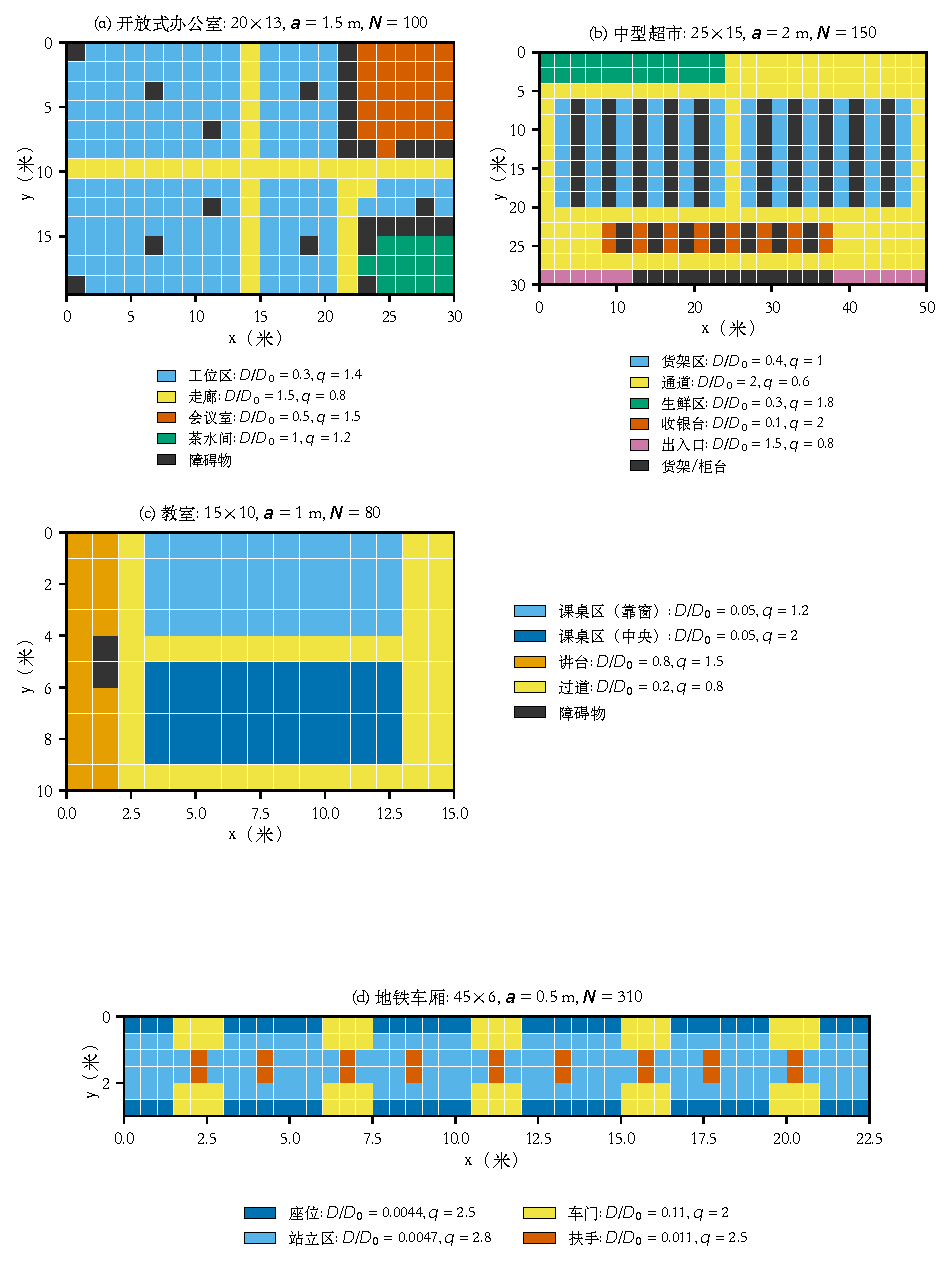
\includegraphics[width=0.84\textwidth]{fig3_scene_maps_zh}
\caption{四个场景的平面布局。每个小方块是一个边长为 $a$ 的格点；颜色标示各分区，其迁移率倍数 $D/\Dz$ 与传染效率
$q$ 见图例；深色格点为障碍物，不属于 $\cells$。各分图标题给出以格点计的格子尺寸、格点间距 $a$ 和人数 $\Npop$。
分区在地面上的布置与分区取值都是示意性假设（见正文）。}
% src: figures/fig3_scene_maps_{en,zh}.pdf, script code/bsc_sim/experiments/20_figures.py (fig_scenes), scenes code/bsc_sim/scenes/*.json
\label{s2_model:fig:scenes}
\end{figure}

模型在四个场景上进行评估：开放式办公室、超市、教室和地铁车厢（表~\ref{s2_model:tab:scenes}，
图~\ref{s2_model:fig:scenes}）。理论与模拟使用同一套场景文件。格子尺寸与格点间距、各分区及其 $d$ 与 $q$ 取值、
人数以及分区在地面上的布置，都是示意性假设；它们既不是测量值，也不是由任何标准推导而来。在办公室中，各分区分别
占地面 260 个格点的 60、15、10、5 和 10\,\%（工位区、走廊、会议室、茶水间和障碍物；234 个可行走格点不含障碍物）；
在超市中，货架与柜台充当障碍物；教室课桌划分为靠窗区块（$q=1.2$）与中央区块（$q=2.0$）；车厢设有车门、座位与
扶手。
% src: code/bsc_sim/scenes/office.json (zone_counts 156, 39, 26, 13, 26 of 260 cells); code/bsc_sim/scenes/supermarket.json, classroom.json, metro.json
地铁的迁移率遵循拥挤规则 $d=c\,n_{\mathrm{d}}^{-\eta}$（站立区 $\eta=2$，其他区域 $\eta=1$），在人群密度
$n_{\mathrm{d}}=310/67.5\,\mathrm{m}^2=4.59$ 人/$\mathrm{m}^2$ 处取值；其面积平均为 $0.028$。
% src: data/s2_model_scenes.json -> scenes.metro (density_used_for_metro_rule_per_m2 4.5926, d_mean 0.0282, zones); code/bsc_sim/scenes/metro.json (D_coef, D_exp)
进入第~\ref{s3_r0:sec}~节上下界的量是 $q$ 在可行走格点上的平均，其值为 $1.300$、$0.914$、$1.318$ 和 $2.536$。
在办公室与超市中，1\,m 接触核就是同格接触核；在教室中，它包含该格点及至多四个相邻格点（平均 $4.6$ 个格点），
在车厢中至多包含 13 个格点（平均 $11.1$ 个）。对这两个场景，同格接触核的结果作为敏感性情形一并报告。
% src: data/s2_model_scenes.json -> scenes.<name>.q_mean; scenes.<name>.kernel1m_cells_mean (1.0, 1.0, 4.62, 11.13), kernel1m_cells_max (1, 1, 5, 13)

\subsection{参数与物理区间}\label{s2_model:sec:regime}

默认的流行病学参数为 $\beta=0.5\perday$ 和 $\gamma=0.14\perday$，对应平均感染期 $7.1$ 天，$\beta/\gamma=3.571$。
它们是示意性取值，未针对任何疾病或数据集进行标定。默认的迁移率尺度 $\Dz=1\cellday$ 同样如此，而这一取值对下文的
每一个结果都有影响。它被用作一个参考性的低迁移率取值，在该取值下模型的空间效应清晰可见；大多数结果也在 $\Dz=10$
与 $100\cellday$ 下给出，各场景在步行迁移率下的 $\Rz$ 亦一并给出（表~\ref{s2_model:tab:regime}）。
% src: data/s2_model_scenes.json -> beta, gamma, beta_over_gamma (3.5714), office_regime.infectious_period_days (7.14)

\paragraph{$\Dz=1$ 意味着什么。}在办公室中（$a=1.5$\,m），$\Dz=1\cellday$ 相当于每天 $2.25\,\mathrm{m}^2$。此时，
$d=1$ 的游走者的均方根位移 $\sqrt{4Dt}$ 在一天内为 $3$\,m，在一个平均感染期内为 $8$\,m，而房间大小为
$30\,\mathrm{m}\times19.5\,\mathrm{m}$。该场景会议室（26 个格点）中的游走者以主离开率 $\muZ=0.00877\perday$ 离开
会议室：其驻留时间 $1/\muZ$ 为 $114$ 天，相当于十六个感染期。在 $\Dz=1$ 的地铁车厢中，乘客平均每天跳跃 $0.075$
次（每次 $0.5$\,m）：在感染期的时间尺度上，车厢是冻结的。
% src: data/s2_model_scenes.json -> office_regime (D0_m2_per_day 2.25, rms_m_per_day_D0 3.0, rms_m_per_infectious_period_D0 8.02), scenes.office.floor_m
% src: data/s2_model_scenes.json -> office_regime (meeting_room_mu_Z_per_day 0.008769, meeting_room_1_over_mu_Z_days 114.04)
% src: data/s2_model_scenes.json -> scenes.metro.hop_rate_mean_per_day_D0=1 (0.0749)

\paragraph{步行迁移率。}对于速度自相关按 $\langle\mathbf{v}(0)\cdot\mathbf{v}(t)\rangle=v^2\e^{-t/\tau}$ 衰减的游走者，
二维扩散系数为 $D=\tfrac12\int_0^\infty\langle\mathbf{v}(0)\cdot\mathbf{v}(t)\rangle\,\dd t=v^2\tau/2$
\citep{taylor1922diffusion,kubo1966fluctuation}。假定步行速度为 $v=1.3\,\mathrm{m\,s^{-1}}$（行人的典型值
\citep{weidmann1993transporttechnik}），并假定持续时间（persistence time）为 $\tau=1.5$\,s，则得
$D=1.27\,\mathrm{m^2\,s^{-1}}$，即在 $a=1.5$\,m 时为 $4.9\times10^{4}\cellday$；若人们只有 5\,\% 的时间在步行，
则为 $2.4\times10^{3}\cellday$。在四个场景中，这些步行取值介于 $1.4\times10^{3}$ 与 $4.4\times10^{5}\cellday$
之间（表~\ref{s2_model:tab:regime}）：$\Dz=1$ 比步行人群的迁移率低三个到接近六个数量级。
% src: data/s2_model_scenes.json -> walking (D_m2_per_s 1.2675), scenes.office (walking_D0_cell2_per_day 48672, walking_5pct_D0_cell2_per_day 2433.6); same values in data/bsc_theory/worked_examples.json -> E9_physical_D
% src: data/s2_model_scenes.json -> scenes.<name>.walking_5pct_D0_cell2_per_day (smallest: supermarket 1368.9), walking_D0_cell2_per_day (largest: metro 438048); log10: 3.14 to 5.64 (data/misc_checks.json -> mobility_gap)

\begin{table}[tbp]
\centering
\caption{本文所用各迁移率尺度 $\Dz$（单位为 \cdunit）及步行迁移率下平均场模型的基本再生数 $\Rz$
（$\beta=0.5\perday$，$\gamma=0.14\perday$）；括号内以及标为“超出量”的列给出 $\Rz$ 超出均匀混合值
$\beta\langle q\rangle/\gamma$ 的百分比。对办公室与超市，1\,m 接触核即同格接触核；对教室与地铁车厢，两种接触核
的结果均列出。$\Dz$ 的步行取值为 $v^2\tau/2$（$v=1.3\,\mathrm{m\,s^{-1}}$，$\tau=1.5$\,s），按各场景的格点间距
换算，分别对应 5\pct{} 的时间在步行和全部时间都在步行的人。}
\label{s2_model:tab:regime}
\footnotesize
% src: data/s2_model_scenes.json -> scenes.<name>.R0_1m, scenes.<name>.R0_samecell (rows as generated in
%      data/s2_model_table_rows.tex); D0 = 1, 10, 100 agree with data/plan_theory_checks.json ->
%      scenes.<name>.R0_1m_D0=*, R0_samecell_D0=*
\setlength{\tabcolsep}{3pt}
\begin{tabular}{@{}llcccccccc@{}}
\toprule
 & & & \multicolumn{3}{c}{$\Rz$（超出量，\%），$\Dz=$}
 & \multicolumn{2}{c}{步行 5\pct{} 时间} & \multicolumn{2}{c}{步行} \\
\cmidrule(lr){4-6}\cmidrule(lr){7-8}\cmidrule(l){9-10}
场景 & 接触核 & $\beta\langle q\rangle/\gamma$ & 1 & 10 & 100 & $\Dz$ & 超出量 & $\Dz$ & 超出量 \\
\midrule
办公室 & 同格 & 4.643 & 5.107 (10.0) & 4.676 (0.72) & 4.646 (0.06) & $2.4\times10^{3}$ & 0.0026 & $4.9\times10^{4}$ & 0.00013 \\
超市 & 同格 & 3.263 & 4.394 (34.6) & 3.391 (3.93) & 3.275 (0.37) & $1.4\times10^{3}$ & 0.0268 & $2.7\times10^{4}$ & 0.00134 \\
教室 & 1\,m & 4.706 & 5.866 (24.7) & 4.931 (4.79) & 4.731 (0.53) & $5.5\times10^{3}$ & 0.0098 & $1.1\times10^{5}$ & 0.00049 \\
 & 同格 &  & 6.182 (31.4) & 4.960 (5.42) & 4.733 (0.57) & $5.5\times10^{3}$ & 0.0105 & $1.1\times10^{5}$ & 0.00053 \\
地铁车厢 & 1\,m & 9.056 & 9.241 (2.1) & 9.164 (1.20) & 9.078 (0.25) & $2.2\times10^{4}$ & 0.0013 & $4.4\times10^{5}$ & 0.00006 \\
 & 同格 &  & 9.836 (8.6) & 9.308 (2.79) & 9.086 (0.33) & $2.2\times10^{4}$ & 0.0016 & $4.4\times10^{5}$ & 0.00008 \\
\bottomrule
\end{tabular}
\end{table}

\paragraph{后果。}在 $\Dz=1$ 时，$q$ 的异质性使 $\Rz$ 比均匀混合值 $\beta\langle q\rangle/\gamma$ 高出 $2$ 至
$35\pct$（1\,m 接触核），具体取决于场景。在步行迁移率下，办公室中的超出量低于 $0.003\pct$，所有场景中均低于
$0.03\pct$：在平均场模型中，有人员步行走动的封闭房间是均匀混合的，就实际应用而言
$\Rz=\beta\langle q\rangle/\gamma$。
% src: data/s2_model_scenes.json -> scenes.<name>.R0_1m.*.excess_over_wellmixed_pct (D0=1: 10.0, 34.6, 24.7, 2.05;
%      walking_5pct: 0.0026, 0.0268, 0.0098, 0.0013; walking: 0.00013, 0.00134, 0.00049, 0.00006);
%      office at D0 = 2400 and 48700 in data/plan_theory_checks.json -> office.mobility_table (0.0027, 0.00013)
第~\ref{s3_r0:sec}--\ref{s6_scenes:sec}~节所报告的封闭房间中的一切空间效应，都只在低迁移率下才较大；
第~\ref{s5_pair:sec}~节的配对层次修正也是如此。经局部的门发生的泄漏是例外：其影响随迁移率增大
（第~\ref{s4_geometry:sec:leaky}~节）。因此，结果针对较低的默认值 $\Dz=1$，以及房间趋近均匀混合极限的 $\Dz=10$
和 $100$ 给出；后续各节将回指本段，不再重复。较小的 $\Dz$ 或可理解为对待在办公桌或座位上的人的一种替代描述，
但不带固定位置的随机游走并不是这类人的恰当模型：慢速游走者会逐渐漂离且不再返回，而且平稳占据在所有可行走格点上
均匀分布，走廊和过道也包括在内。第~\ref{s8b_evidence:sec:contacts}~节以实测接触为对照展示了这一后果，所用迁移率
与实测接触时长相匹配：按六个室内场所中接触的总量与时长标定的自由游走，在六个场所中的五个使每个人的接触对象过多，
且在任何一个场所中都没有群组结构。

\paragraph{封闭房间。}除非另有说明，每个场景都是一个封闭房间，在整个流行过程中由同样的 $\Npop$ 个人每天 24 小时
占据。这对办公室和教室是一种理想化；对超市和地铁车厢则不是一个现实的物理情形，场景文件为二者分别假定了 27 分钟和
20 分钟的到访；
% src: code/bsc_sim/scenes/supermarket.json, metro.json ("dwell")
第~\ref{s6_scenes:sec:interventions}~节给出了每次到访以及每天只有部分时间被占用的房间所对应的数值。

% m3_r0.tex -- Main text, Section 3: the basic reproduction number of the mean-field model.
% Proofs are in the Supplementary Material (supp_r0.tex); they follow code/bsc_theory/scripts and the
% derivations checked there, in the article's notation (cells x, y; column index = source cell).
% Numbers: data/plan_theory_checks.json (canonical scenes; code/plan_theory_checks.py) and
% data/s3_r0_checks.json (written by code/s3_r0_checks.py, which recomputes them with
% other code and agrees with the first file to 2e-14).
% Paths in "% src:" comments are relative to the repository root.
\section{平均场模型的基本再生数}\label{s3_r0:sec}

本节确定平均场模型~\eqref{s2_model:eq:meanfield} 的基本再生数 $\Rz$、它的上下界及其对迁移率的依赖关系。本节始终在
假设~\ref{s2_model:ass:A} 下讨论，记 $\Vm=\gamma\Id-\gen$，矩阵的列指标对应源格点，向量或矩阵之间的不等式均按逐元素
理解。每条结论都注明了它所需要的接触核：多数结论要求同格接触核 $\Fm=\beta\Qm$，其中 $q\ge0$，$q\not\equiv0$。
主要结果对传染病斑块模型而言是已知的（第~\ref{s1_intro:sec}~节，表~\ref{s1_intro:tab:known}），本文不主张其新颖性。
补充材料第~\ref{S-appS_r0:sec}~节从非负矩阵的标准结论出发给出了完整证明，因为证明确定了每条结论成立的条件（哪种
接触核、跳跃率具有何种对称性）。分区下界、慢混合系数和逐边单调性都是同一矩阵理论的初等推论；一次定向检索
（2026 年 10 月 1 日在 Crossref 上就斑块模型的再生数与扩散所做的查询）未找到它们的出处，但这并不能证明不存在出处。
% src: data/refs_search.json (searches; manual_checks: gao2020fast, tien2015disease, allen2007asymptotic)

\begin{theorem}[下一代矩阵]\label{s3_r0:thm:ngm}
  在假设~\ref{s2_model:ass:A} 下，设 $\Fm\ge0$，$\Fm\neq0$，$\Vm=\gamma\Id-\gen$，并定义
  \begin{equation}\label{s3_r0:eq:ngm}
     \ngm=\Fm\Vm^{-1},\qquad \Rz=\srad(\ngm),\qquad \lamone=\sabs(\Jm),\quad \Jm=\gen+\Fm-\gamma\Id .
  \end{equation}
  \begin{enumerate}[label=\textup{(\alph*)},leftmargin=*]
    \item 逐元素地有 $\Vm^{-1}=\int_0^\infty \e^{-\gamma t}\e^{\gen t}\,\dd t>0$。对 $\Fm=\beta\ker^{\T}\Qm$，
      $K_{yx}=\beta\sum_{z}P_{zy}\,q_z\int_0^\infty \e^{-\gamma t}P_t(z\,|\,x)\,\dd t$ 是在完全易感的房间中、于格点 $x$
      引入的一个感染者在格点 $y$ 所造成感染的期望数；对同格接触核，
      $K_{yx}=\beta q_y\int_0^\infty \e^{-\gamma t}P_t(y\,|\,x)\,\dd t$。
    \item $\Rz>0$，且 $\Rz$ 是满足 $\sabs(\gen+\Fm/R-\gamma\Id)=0$ 的唯一 $R>0$。
    \item $\lamone<0\iff\Rz<1$，$\lamone=0\iff\Rz=1$，$\lamone>0\iff\Rz>1$。
    \item 式~\eqref{s2_model:eq:meanfield} 的每个解对所有 $t\ge0$ 逐分量满足 $I(t)\le \e^{\Jm t}I(0)$。因此，若
      $\Rz<1$，则感染者人数从 $t=0$ 起即以一个衰减指数函数为上界：$\one^{\T}I(t)\le C\,\e^{\lamone t}\,\one^{\T}I(0)$，
      其中 $\lamone<0$，且 $C$ 与初始条件无关。若 $\Rz>1$，则无病平衡态不稳定，线性化解按 $\e^{\lamone t}$ 增长。
  \end{enumerate}
\end{theorem}

在封闭的 SIR 模型中，无论 $\Rz$ 取何值，感染者最终都会消失；(d) 的内容在于：当 $\Rz<1$ 时，任何时刻都不会出现
增长，而当 $\Rz>1$ 时，少量初始感染会增长，直到易感者的耗竭使其停止。$\ngm$ 的列和是在格点 $x$ 引入的指示病例
所致二代病例的期望数，即后代数 $\noff(x)$；对每个行随机的接触核，
\begin{equation}\label{s3_r0:eq:offspring}
  \noff(x)=\sum_yK_{yx}=\beta\,\Exp_x\!\int_0^{\tau}q(X_t)\,\dd t ,\qquad
  \frac{\beta\qmin}{\gamma}\le\noff(x)\le\frac{\beta\qmax}{\gamma},\qquad \sum_x\pi_x\noff(x)=\frac{\beta\qmean}{\gamma},
\end{equation}
其中 $X_t$ 是从 $x$ 出发的游走，$\tau$ 是其服从指数分布的感染期。在 $\Dz=1\cellday$ 的办公室场景中，$\noff(x)$ 在
各格点上的取值范围为 $3.995$ 至 $5.335$，其均匀平均值为 $4.643$。
% src: data/plan_theory_checks.json: office/D0=1/offspring_min, offspring_max, offspring_uniform_mean
下一代矩阵为 $\ngm=\Fm\,\widehat G(\gamma)$，其中 $\widehat G(\gamma)=(\gamma\Id-\gen)^{-1}$ 是格点传播子的拉普拉斯
变换在恢复率处的取值；对可逆移动，$\Rz$ 还有一个变分（瑞利）形式，以及一个以移动生成元的特征模态表示的模态矩阵
形式，其最大的对角元只是一个下界（补充材料定理~\ref{S-s3_r0:thm:rayleigh} 与推论~\ref{S-s3_r0:cor:modal}）。

\begin{theorem}[上下界；同格接触核]\label{s3_r0:thm:bounds}
  在假设~\ref{s2_model:ass:A} 下，设 $\Fm=\beta\Qm$，其中 $q\ge0$，$q\not\equiv0$。则对每个不可约生成元（无论可逆
  与否），
  \begin{equation}\label{s3_r0:eq:bounds}
    \frac{\beta\qmean}{\gamma}\le\Rz\le\frac{\beta\qmax}{\gamma},\qquad
    \beta\qmean-\gamma\le\lamone\le\beta\qmax-\gamma .
  \end{equation}
  若 $q$ 为常数，则四处均取等号；若 $q$ 不为常数，则四个不等式均严格成立。
\end{theorem}

由式~\eqref{s3_r0:eq:offspring}，$\beta\qmean/\gamma$ 是按平稳分布放置的指示病例所致二代病例的平均数。$\Rz$ 之所以
更大，是因为二代病例并非按平稳分布产生：它们优先产生于 $q$ 高的格点，并在那里开始其感染期。迁移会抹去这种对出生地
的记忆（定理~\ref{s3_r0:thm:mobility}）。因此，在同格接触核下，不存在任何机制能使空间隔离把平均场 $\Rz$ 降到均匀
混合值 $\beta\qmean/\gamma$ 以下；空间隔离对离散个体有何作用，则是另一个问题（第~\ref{s5_pair:sec}~节和
第~\ref{s6_scenes:sec}~节）。

\begin{theorem}[迁移率；同格接触核]\label{s3_r0:thm:mobility}
  设 $\gen=\Dz\genz$，其中 $\genz$ 是平稳分布为 $\stat$ 的不可约生成元，且 $\Fm=\beta\Qm$。则
  \begin{enumerate}[label=\textup{(\alph*)},leftmargin=*]
    \item $\lim_{\Dz\to\infty}\Rz(\Dz)=\beta\qmean/\gamma$；
    \item $\lim_{\Dz\to0^+}\Rz(\Dz)=\beta\qmax/\gamma$；
    \item $\lamone(\Dz)$ 是凸的且单调不增，$\Rz(\Dz)$ 单调不增；若 $q$ 不为常数，则 $\Rz(\Dz)$ 在 $(0,\infty)$ 上
      严格递减。
  \end{enumerate}
  本定理不需要可逆性。
\end{theorem}

\begin{proposition}[渐近展开]\label{s3_r0:prop:expansions}
  在定理~\ref{s3_r0:thm:mobility} 的条件下：
  \begin{enumerate}[label=\textup{(\roman*)},leftmargin=*]
    \item 当 $\Dz\to\infty$ 时，$\Rz(\Dz)=\dfrac{\beta\qmean}{\gamma}+\dfrac{\beta\,C}{\qmean\,\Dz}+O(\Dz^{-2})$，其中
      $C=\qvec^{\T}\mathbf{y}\ge0$，$\mathbf{y}$ 满足 $-\genz\mathbf{y}=\Qm\stat-\qmean\stat$，$\one^{\T}\mathbf{y}=0$
      （速率对称时，$C=\ncell^{-1}\,\delta q^{\T}(-\genz)^{+}\delta q$，其中 $\delta q=\qvec-\langle q\rangle\one$，
      $(\cdot)^{+}$ 表示伪逆）；
    \item 当 $\Dz\to0$ 时，$\Rz(\Dz)=\dfrac{\beta\qmax}{\gamma}\Bigl(1-\dfrac{\Dz\,\mu^0_Z}{\gamma}\Bigr)+o(\Dz)$，其中
      $Z=\{x:q_x=\qmax\}$，$\mu^0_Z=-\sabs(\genz[Z,Z])$。
  \end{enumerate}
\end{proposition}

\begin{proposition}[分区下界]\label{s3_r0:prop:zone}
  在假设~\ref{s2_model:ass:A} 下，设 $\Fm=\beta\Qm$。则对每个非空的 $Z\subset\cells$，
  \begin{equation}\label{s3_r0:eq:zone}
    \Rz\ \ge\ \frac{\beta\,q_Z}{\gamma+\muZ},\qquad q_Z=\min_{x\in Z}q_x,\qquad \muZ=-\sabs(\gen[Z,Z])\ge0 .
  \end{equation}
\end{proposition}

其中 $\muZ$ 是一旦走出 $Z$ 即消亡的游走者的主衰减率。由命题~\ref{s3_r0:prop:expansions}(ii)，取
$Z=\{x:q_x=\qmax\}$ 的分区下界在 $\Dz\to0$ 时精确到一阶。因此，形如 $\beta q/(\gamma+\mu)$ 的表达式在封闭房间中确实
会出现，但它是一个下界，由一个高风险分区贡献，感染者会从该分区逃入风险较低的空间；式中的 $q$ 和 $\mu$ 是该分区的
量，而不是整个房间的量。

\begin{theorem}[逐边单调性；对称速率，同格接触核]\label{s3_r0:thm:edges}
  若对所有连边有 $\hop{x}{y}=\hop{y}{x}$，且 $\Fm=\beta\Qm$，则 $\Rz$ 与 $\lamone$ 都是每一条连边速率的单调不增函数。
  因此，在规则~\eqref{s2_model:eq:hop} 下并对固定的格点集合 $\cells$，降低任意一组格点中的 $D$ 或封闭连边（在格点
  之间设墙）都不能降低 $\Rz$。
\end{theorem}

该定理只涉及保持格点集合不变的操作。把格点变为障碍格，会将这些格点及其 $q$ 从 $\cells$ 中移除；这会改变 $\qmean$
以及定理~\ref{s3_r0:thm:bounds} 的两个界，此时 $\Rz$ 可能下降（第~\ref{s4_geometry:sec:examples}~节）。对称性是
必不可少的：在出发点规则下，改变 $D$ 也会改变平稳占据分布；在 $300$ 个随机算例中，将某一个格点的 $D$ 乘以 $3$，
有 $201$ 个算例的 $\Rz$ 上升，$98$ 个下降，一个不变（在 $10^{-10}$ 的精度内）。
% src: data/bsc_theory/verify_theorems.json: T3p/departure_up, departure_down

\begin{proposition}[接触核]\label{s3_r0:prop:kernel}
  设 $\Fm=\beta\ker^{\T}\Qm$，其中 $\ker$ 为行随机矩阵。则
  \begin{enumerate}[label=\textup{(\roman*)},leftmargin=*]
    \item 定理~\ref{s3_r0:thm:ngm} 成立；
    \item $\beta\qmin/\gamma\le\Rz\le\beta\qmax/\gamma$，且若 $q\equiv q_0$，则 $\Rz=\beta q_0/\gamma$；
    \item 当 $\Dz\to\infty$ 时 $\Rz(\Dz)\to\beta\qmean/\gamma$，当 $\Dz\to0$ 时 $\Rz(\Dz)\to\srad(\beta\ker^{\T}\Qm)/\gamma$；
    \item 定理~\ref{s3_r0:thm:bounds} 的下界 $\beta\qmean/\gamma\le\Rz$ 和定理~\ref{s3_r0:thm:mobility}(c) 的单调性都可能
      不成立。例：排成一行的三个格点，相邻格点之间的跳跃率为 $\Dz$，$\ker$ 在一个格点及其相邻格点上均匀分布，
      $q=(1,0,1)$：则 $\Rz(\Dz)=(\beta/\gamma)(\gamma+4\Dz)/(2\gamma+6\Dz)$，它在 $\Dz=0$ 时为 $0.5\,\beta/\gamma$，
      低于 $\beta\langle q\rangle/\gamma=0.667\,\beta/\gamma$，且随 $\Dz$ 增大而增大。
  \end{enumerate}
\end{proposition}
% src: data/plan_theory_checks.json: checks/kernel_counterexample_q=[1.0, 0.0, 1.0] (0.500, 0.503, 0.529,
%      0.614, 0.659, 0.666, 0.6667 at D0 = 0, 0.001, 0.01, 0.1, 1, 10, 1000 with gamma = 0.14);
%      closed form checked to 8e-14 in data/s3_r0_checks.json: kernel_closed_form_max_abs_diff

在接触核下，位于高 $q$ 格点的感染者会感染相邻格点中的人；若这些格点的 $q$ 较低且无人移动，新病例就很少再传播，
于是在同格接触核下抬高 $\Rz$ 的规模偏倚发生了逆转。在本文中 1\,m 接触核与同格接触核不同的两个场景里，该下界恰好
成立（在 $\Dz=1\cellday$ 时，教室中为 $5.866\ge4.706$，地铁车厢中为 $9.241\ge9.056$），但这并无保证。
% src: data/plan_theory_checks.json: scenes/classroom, scenes/metro (R0_1m_D0=1, lower)

\subsection{场景}\label{s3_r0:sec:scenes}

\begin{figure}[tbp]
  \centering
  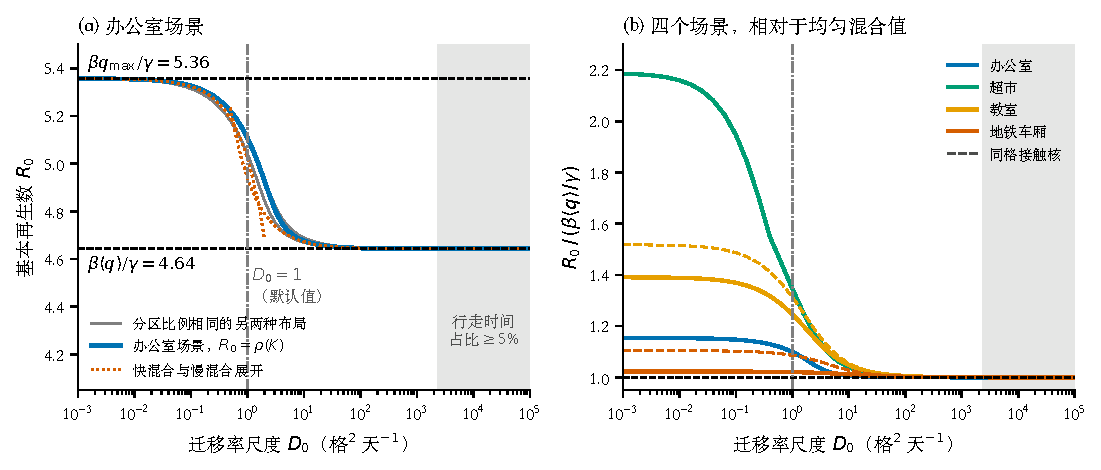
\includegraphics[width=\textwidth]{fig_r0_mobility_zh}
  \caption{平均场基本再生数 $\Rz=\srad(\ngm)$ 随迁移率尺度 $\Dz$（\cdunit）的变化，$\beta=0.5\perday$，
  $\gamma=0.14\perday$；$\Rz$ 与人数 $\Npop$ 无关（频率依赖发生率），且不涉及任何模拟。
  (a)~办公室场景（234 个可行走格点，同格接触核）：$\Rz$（粗线）、定理~\ref{s3_r0:thm:bounds} 的上下界
  $\beta\langle q\rangle/\gamma$ 与 $\beta\qmax/\gamma$（虚线）、命题~\ref{s3_r0:prop:expansions} 的两个渐近展开（点线），
  以及分区比例相同的另两种平面布局（细灰线）。(b)~四个场景，以 $\Rz$ 与均匀混合值 $\beta\langle q\rangle/\gamma$
  之比表示，分别采用 1\,m 接触核（实线）和同格接触核（虚线；对办公室和超市二者重合）。点划竖线标出默认值
  $\Dz=1$；阴影带为 $\Dz\ge2.4\times10^{3}$，就办公室的格点间距（$a=1.5$\,m）而言，这是至少有 5\pct{} 的时间在步行的
  人的迁移率（第~\ref{s2_model:sec:regime}~节；其他场景的相应取值见表~\ref{s2_model:tab:regime}）。}
  % src: code/plan_fig_theory.py (fig_r0_mobility) <- data/plan_theory_checks.json, plan_theory_sweeps.npz
  \label{s3_r0:fig:mobility}
\end{figure}

对具有办公室场景分区比例（$\langle q\rangle=1.300$，$\qmax=1.5$）的任何平面布局，定理~\ref{s3_r0:thm:bounds} 都给出
$4.643\le\Rz\le5.357$。在该场景本身中，$\Dz=1\cellday$ 时 $\Rz=5.107$，增长率 $\lamone=0.602\perday$（倍增时间
$1.15$ 天）；分区比例相同的另两种平面布局分别给出 $5.109$ 和 $5.041$。
% src: data/plan_theory_checks.json: office/lower_bound, upper_bound, q_mean, q_max
% src: data/plan_theory_checks.json: office/D0=1 (R0, lambda1, doubling_time); alternative_layouts/O1, O2 (R0_D0_1)
曲线 $\Rz(\Dz)$ 从上界递减至下界（图~\ref{s3_r0:fig:mobility}(a)），命题~\ref{s3_r0:prop:expansions} 的两个渐近展开为
$\Rz\simeq4.643+0.296/\Dz$（$\Dz\to\infty$）和 $\Rz\simeq5.357\,(1-0.0626\,\Dz)$（$\Dz\to0$；$\Dz$ 的单位为 \cdunit）。
第一个展开在 $\Dz=10$ 处精确到 $0.004$，在 $\Dz=100$ 处精确到 $3\times10^{-5}$；第二个展开在 $\Dz=0.1$ 处精确到
$0.003$。
% src: data/plan_theory_checks.json: office/largeD_coefficient_betaC_over_qbar, office/smallD_slope_muZ0_over_gamma
% src: data/s3_r0_checks.json: office/expansions/rows (err_fast, err_slow)
慢混合展开中的集合 $Z$ 是会议室（26 个格点，$q=1.5$），其在 $\Dz=1$ 时的拟平稳驻留时间为 $1/\muZ=114$ 天；其分区
下界~\eqref{s3_r0:eq:zone} 为 $5.041$。这些都是该平面布局的性质：在这一布局中，会议室只通过一个格点与走廊相连。
% src: data/plan_theory_checks.json: office/zone_bound_meeting_room (mu_Z, exit_time_days, bound, cells)
在四个场景中，$\Dz=1$ 时 $\Rz$ 相对于均匀混合值的超出量在超市中最大（$+34.6\pct$），该场景的 $\qmax$ 是 $\langle q\rangle$ 的
两倍以上（表~\ref{s2_model:tab:regime}，图~\ref{s3_r0:fig:mobility}(b)）。
% src: data/s3_r0_checks.json: scenes/supermarket/D0=1/excess_1m_pct

对于在 $20\times13$ 格子上由工作区（$q_W=1.5$，$D=0.3\,\Dz$）和中央走廊带（$q_C=0.5$，$D=2\,\Dz$）组成、
$\langle q\rangle=1.2$ 的两区房间，定理~\ref{s3_r0:thm:bounds} 给出 $\Rz\ge1.2\,\beta/\gamma$：把低风险走廊与高风险
工作区隔开，不能降低平均场 $\Rz$。数值上，$\Dz=1$ 时 $\Rz=4.972=1.39\,\beta/\gamma$，$\Dz=10$ 时为
$1.24\,\beta/\gamma$，$\Dz\ge100$ 时为 $1.20\,\beta/\gamma$。同样两个分区的另外四种排布（工作区占 $69$--$70\pct$）在
$\Dz=1$ 时给出 $1.43\,\beta/\gamma$（走廊带沿一面墙）和 $1.22$--$1.23\,\beta/\gamma$（过道、过道网格、分散的走廊
格点）：两个分区交错得越细，$\Rz$ 就越接近均匀混合值。
% src: data/bsc_sim/05_heterogeneity.json: "D0=1|N=100|c=0.5833"/R0_ngm = 4.972; data/s3_r0_checks.json: two_zone/rows (1.3922, 1.2395, 1.2043, 1.2004)
% src: data/bsc_theory/worked_examples.json: E1_two_zone/{side,aisles,grid,scatter}/symmetric/R0_over_beta_gamma
%      (1.425, 1.224, 1.221, 1.227; workspace 180/260 or 182/260 cells)

本节的每一条结论都在四族生成元的随机算例上做了检验，复核中还重新推导了各项证明、重新实现了各项计算（补充
材料第~\ref{S-appA_numerics:sec:theorems}~节）；例如，在 $2{,}000$ 个随机算例中，上下界~\eqref{s3_r0:eq:bounds} 的
最大违反量为 $4\times10^{-14}$，处于舍入误差的量级。
% src: data/bsc_theory/verify_theorems.json: T2 (n_instances 2000, max_viol_upper 4.0e-14, max_viol_lower 2.3e-15)

% m4_geometry.tex -- Main text, Section 4: Room size, leaks and hotspot maps.
% Paths in "% src:" comments are relative to the repository root.
% Numbers come from  data/plan_theory_checks.json (canonical office scene, written by
% code/plan_theory_checks.py),  data/bsc_theory/worked_examples.json and
% fig2_room_size_data.json (room size, leaks; written by code/bsc_theory/scripts/worked_examples.py
% and make_figures.py),  data/s4_geometry_checks.json (derived numbers and a second computation;
% written by code/s4_geometry_checks.py), data/s4_geometry_barriers_leak.json and
% data/s4_geometry_leak_kernels.json.  Proofs: Supplementary Section S3.
\section{房间尺寸、泄漏与热点分布图}\label{s4_geometry:sec}

第~\ref{s3_r0:sec}~节表明，迁移率与 $q$ 的异质性共同把 $\Rz$ 限定在 $\beta\qmean/\gamma$ 与 $\beta\qmax/\gamma$ 之间。
本节考察房间的几何形状还会带来哪些影响。本节内容均不作为新结果提出：定理~\ref{s4_geometry:thm:closed} 的不变性对于
各斑块再生数相等的斑块模型是已知的\citep{gao2011sis}；经吸收边界的流失即 Skellam 的临界斑块尺寸机制
\citep{skellam1951random,cantrell2003spatial}；定理~\ref{s4_geometry:thm:leaky} 中的拟平稳对象可追溯到
\citet{darroch1967quasi}；定理~\ref{s4_geometry:thm:hotspots} 则是 Perron--Frobenius 理论与单重特征值灵敏度的结合
\citep{berman1994nonnegative,horn2013matrix}。对于此处所述的泄漏房间表述，我们不知道有任何出处；我们只检索了
第~\ref{s1_intro:sec}~节中的斑块模型结果。证明见补充材料第~\ref{S-appS_geometry:sec}~节。

\subsection{封闭房间：不存在有限尺寸效应}\label{s4_geometry:sec:closed}

\begin{theorem}[封闭房间，均匀 $q$]\label{s4_geometry:thm:closed}
  在假设~\ref{s2_model:ass:A} 下，设 $q\equiv q_0$，且 $\Fm=\beta\ker^{\T}\Qm$，其中接触核为任意行随机矩阵。则对任意
  房间尺寸、形状、障碍物布局、迁移率场与迁移率尺度，均有 $\Rz=\beta q_0/\gamma$ 和 $\lamone=\beta q_0-\gamma$；并且在
  平均场模型中，每个指示病例无论从何处开始，所致二代病例数的期望均为 $\noff(x)=\beta q_0/\gamma$。
\end{theorem}

反射壁不会损失任何人：$\ngm$ 的各列和均等于 $\beta q_0/\gamma$。等价地，对均匀 $q$，补充材料
推论~\ref{S-s3_r0:cor:modal} 的模态矩阵是对角矩阵，对角元为 $\beta q_0/(\gamma+\mu_j)$，其中最大者是均匀模态
（$\mu_0=0$）对应的元素；边长为 $L$（格）的方形房间的第一个非零特征值 $\mu_1=2D[1-\cos(\pi/L)]\approx\pi^2D/L^2$
不起任何作用。$L=3,\dots,40$、$D=0.5\cellday$ 的方形房间给出 $\srad(\ngm)=\beta q/\gamma$，相对误差在
$6\times10^{-15}$ 以内；40 个随机房间（含障碍格，迁移率跨越四个数量级，生成元既有对称的也有非对称的，接触核随机
选取）均在 $10^{-13}$ 以内再现了 $\Rz=\beta q_0/\gamma$、$\lamone=\beta q_0-\gamma$ 和 $\noff(x)=\beta q_0/\gamma$。
因此，在封闭房间中，几何形状只通过迁移率与 $q$ 的异质性之间的相互作用进入 $\Rz$。
% src: data/bsc_theory/fig2_room_size_data.json (refl: max |ratio-1| = 5.8e-15);
% src: data/s4_geometry_checks.json: B_closed_room_general_kernel (1.9e-14, 1.8e-14, 6.5e-14)

\subsection{泄漏房间}\label{s4_geometry:sec:leaky}

真正的边界效应要求人员会离开。设位于格点 $x$ 的人以速率 $\kappa_x\ge0$ 离开房间（经由门格、敞开的一侧，
或在一段与位置无关的停留时间之后），并立即由一名从同一格点进入的易感者替换，使占据人数保持为 $N^*$；只计入
发生在房间内的感染。于是感染者遵循生成元为 $\genk=\gen-\diag\kappa$ 的带消亡的游走。

\begin{theorem}[泄漏房间；同格接触核]\label{s4_geometry:thm:leaky}
  在假设~\ref{s2_model:ass:A} 下，设 $\Fm=\beta\Qm$，$\kappa\ge0$，$\kappa\not\equiv0$，并令
  $\genk=\gen-\diag\kappa$，$\Vm_\kappa=\gamma\Id-\genk$，$\Rroom=\srad(\beta\Qm\Vm_\kappa^{-1})$，
  $\muk=-\sabs(\genk)$。设 $\uvec_\kappa,\lvec_\kappa>0$ 为 $\genk$ 的右、左 Perron 向量，且
  $\nu=(\lvec_\kappa\circ\uvec_\kappa)/(\lvec_\kappa^{\T}\uvec_\kappa)$。则
  \begin{enumerate}
    \item[(1)] 将 $\gen$ 替换为 $\genk$ 后，定理~\ref{s3_r0:thm:ngm}(a)--(c) 仍成立；
    \item[(2)] $0<\muk\le\langle\kappa\rangle_\pi:=\sum_x\pi_x\kappa_x$；$\muk$ 关于每个 $\kappa_x$ 单调不减；并且对
       门集合 $\Delta\subsetneq\cells$ 与 $\kappa=k\,\one_\Delta$，当 $k\to\infty$ 时
       $\muk\uparrow\mu^{\mathrm{abs}}_\Delta:=-\sabs(\gen[\cells\setminus\Delta,\cells\setminus\Delta])$；
    \item[(3)] 若 $q\equiv q_0$，则 $\Rroom=\beta q_0/(\gamma+\muk)$；
    \item[(4)] 一般地，$\beta\langle q\rangle_\nu/(\gamma+\muk)\le\Rroom\le\beta\qmax/(\gamma+\muk)$，其中
       $\langle q\rangle_\nu=\sum_x\nu_xq_x$。
  \end{enumerate}
\end{theorem}

$\uvec_\kappa$ 是条件于仍在房间内的游走者的拟平稳分布\citep{darroch1967quasi}，$1/\muk$ 是其渐近平均驻留时间，
$\nu$ 则是条件于永不离开的游走的平稳分布。当 $\kappa\to0$ 时，$\nu\to\stat$，(4) 退化为
定理~\ref{s3_r0:thm:bounds}。有两种情形可以显式求解。

\begin{corollary}[显式情形]\label{s4_geometry:cor:cases}
  \emph{(a) 均匀泄漏（停留时间）。} 若 $\kappa_x\equiv1/T$，则 $\muk=1/T$，$\nu=\stat$，并且
  第~\ref{s3_r0:sec}~节中关于同格接触核的每个结果，在把 $\gamma$ 替换为 $\gamma+1/T$ 后都对 $\Rroom$ 成立；特别地，
  \begin{equation}\label{s4_geometry:eq:dwell}
     \frac{\beta\qmean\,T}{1+\gamma T}\;\le\;\Rroom\;\le\;\frac{\beta\qmax\,T}{1+\gamma T},
  \end{equation}
  并且在服从 $\stat$ 分布的位置进入房间的感染者，在房间内所致感染数的期望为 $\beta\qmean T/(1+\gamma T)$。对任意
  行随机接触核，令 $\Rroom:=\srad(\beta\ker^{\T}\Qm\Vm_\kappa^{-1})$，则第~\ref{s3_r0:sec}~节中对该接触核成立的每个
  结果，在把 $\gamma$ 替换为 $\gamma+1/T$ 后都对 $\Rroom$ 成立；特别地，当 $q\equiv q_0$ 时
  $\Rroom=\beta q_0/(\gamma+1/T)$。

  \emph{(b) 两端吸收的走廊。} 对排成一行的 $L$ 个格点，相邻格点间的跳跃率为 $w$，$q$ 均匀，两个端格上
  $\kappa=w$（越过任一端的跳跃即离开房间），有
  \begin{equation}\label{s4_geometry:eq:corridor}
     \muk=2w\Bigl[1-\cos\frac{\pi}{L+1}\Bigr]=\frac{\pi^2w}{(L+1)^2}+O\bigl(wL^{-4}\bigr),\qquad
     \Rroom=\frac{\beta q}{\gamma+2w\bigl[1-\cos\frac{\pi}{L+1}\bigr]} .
  \end{equation}
\end{corollary}

设格点间距为 $a$，$w=D/a^2$，物理长度为 $\ell=La$，则式~\eqref{s4_geometry:eq:corridor} 趋于
$\beta q/(\gamma+\pi^2D/\ell^2)$；因此，这是两端为\emph{吸收}端的走廊的再生数，而不是封闭房间的再生数。其机制即
空间生态学中的临界斑块尺寸\citep{skellam1951random,cantrell2003spatial}：速率为 $\beta q-\gamma$ 的增长与速率为
$\muk$ 的边界流失相互竞争，只有当走廊长度大于约 $\pi\sqrt{D/(\beta q-\gamma)}$ 时才有 $\Rroom>1$。取
$w=1\perday$、$\beta q=0.5\perday$，这一连续估计为 $5.2$ 格；在格点上，$\Rroom$ 在 $L=5$ 时首次超过 1（$L=4$ 时为
$0.958$，$L=5$ 时为 $1.226$）。
% src: data/bsc_theory/fig2_room_size_data.json: L1, r1 (L = 4, 5);
% src: data/s4_geometry_checks.json: A_room_size_and_leaks/corridor_critical_L_continuum (5.236)

门为局部时，第 (3)、(4) 部分不能推广到其他接触核：在一端设门的三格点例子中，对最近邻接触核，第 (3) 部分的
公式偏差 $-3.0\,\%$；对一个偏斜的接触核，在两种门位置之一下，$\Rroom$ 比第 (4) 部分的上界高出 $10.9\,\%$（补充
材料注~\ref{S-s4_geometry:rem:kernels}）。对异质 $q$ 和局部的门，替换 $\gamma\to\gamma+\muk$ 也不精确：在办公室
场景中，于一条走廊支路的末端设一个 $\kappa=100\perday$ 的门、取 $\Dz=10$，得 $\Rroom=4.220$，而替换给出 $4.133$，
低于第 (4) 部分的下界 $4.139$；原因在于，位于低 $q$ 分区的门使条件于留在房间内的游走偏向较高的 $q$。
% src: data/s4_geometry_leak_kernels.json (a_uniform_q_neighbour_kernel_end_door: -2.99 %; b_uniform_q_skew_kernel_end_door: excess 10.91 %)
% src: data/s4_geometry_barriers_leak.json: B_leak_heterogeneous_q/cases/"D0=10|kappa=100" (R_room 4.2201, R_substitution 4.1331, lower_bound 4.1386)

泄漏会降低再生数，房间越小降幅越大（补充材料图~\ref{S-s4_geometry:fig:leak}(a)）。有两点需要注意。第一，在
$D=0.5\cellday$ 时，这些泄漏率很小（$\muk\le0.1\perday$，驻留时间介于 $10$ 天与 $19$ 年之间）。对于固定的几何形状
和离开率本身就是一个跳跃率的门（$\kappa=D$），$\muk$ 与迁移率尺度成正比，因此在 $D=2.4\times10^{3}\cellday$ 时
（第~\ref{s2_model:sec:regime}~节），同样的驻留时间将介于 $3$ 分钟与 $1.5$ 天之间。离开率 $\kappa$ 固定的门则表现
不同：其泄漏率随迁移率增大，但始终低于 $\langle\kappa\rangle_\pi$；在设一个门格、$\kappa=1\perday$ 的办公室中，
$\Dz=1$、$10$、$100$ 和 $2{,}400$ 时 $\Rroom/\Rz$ 分别为 $0.99998$、$0.977$、$0.971$ 和 $0.970$。因此在应用中，停留
时间 $T$ 应作为输入给定（如推论~\ref{s4_geometry:cor:cases}(a)），而不应是走向门的随机游走的输出。
% src: data/s4_geometry_checks.json: A_room_size_and_leaks/residence_days_range_D0.5 (10.1 d, 7041 d = 19.3 yr),
%      max_mu_D0.5 (0.099), residence_range_at_D2400 (3.0 min, 1.47 d); data/s4_geometry_leak_kernels.json
%      (d_office_door_against_mobility: fixed_kappa_1 R_room_over_R0 0.99998, 0.977, 0.971, 0.970)
第二，$\Rroom$ 计的是一次停留期间的感染数。每天都回到同一房间的感染者在一个感染期内会有多次停留，因此按每次
到访计的数并不是被反复到访的场所的再生数；日内作息安排在第~\ref{s6_scenes:sec:interventions}~节中讨论。

\subsection{热点分布图}\label{s4_geometry:sec:hotspots}

\begin{theorem}[热点分布图；同格接触核]\label{s4_geometry:thm:hotspots}
  在假设~\ref{s2_model:ass:A} 下，设 $\Fm=\beta\Qm$，且对所有 $x$ 有 $q_x>0$。设 $\uvec,\lvec>0$ 为 $\Jm$ 的
  右、左 Perron 向量（$\one^{\T}\uvec=1$），$\wvec,\zvec>0$ 为 $\ngm$ 的右、左 Perron 向量
  （$\ngm\wvec=\Rz\wvec$，$\zvec^{\T}\ngm=\Rz\zvec^{\T}$，$\one^{\T}\wvec=1$），并设 $\xi>0$ 满足
  $\beta\Qm\xi=\Rz(\gamma\Id-\gen)\xi$。
  \begin{enumerate}
    \item[(i)] （现患）对每个 $\delta'<\delta$，有
       $\e^{\Jm t}I(0)=\e^{\lamone t}\bigl[(\lvec^{\T}I(0)/\lvec^{\T}\uvec)\,\uvec+O(\e^{-\delta' t})\bigr]$，其中
       $\delta=\lamone-\max\{\operatorname{Re}\lambda:\lambda\in\sigma(\Jm)\setminus\{\lamone\}\}>0$；若 $\Jm$
       可对角化（特别是对可逆移动），可取 $\delta'=\delta$。$\uvec\propto\stat$ 当且仅当 $q$ 为常数。
    \item[(ii)] （发病）当 $g\to\infty$ 时，$\ngm^{g}I_0=\Rz^{g}\bigl[(\zvec^{\T}I_0/\zvec^{\T}\wvec)\,\wvec+o(1)\bigr]$；
       $\wvec\propto\Qm\xi$；并且按 $\stat$ 放置的指示病例所产生的第一代感染为
       $(\ngm\stat)_x=\beta q_x\pi_x/\gamma$。
    \item[(iii)] （弹性）$e_x:=\partial\ln\Rz/\partial\ln q_x=z_xw_x/(\zvec^{\T}\wvec)\ge0$，且 $\sum_xe_x=1$。
       对可逆移动，$\zvec\propto\Pi^{-1}\xi$，$\Pi=\diag\stat$，且 $e_x\propto q_x\xi_x^2/\pi_x$。
    \item[(iv)] （极限）设 $\gen=\Dz\genz$。当 $\Dz\to\infty$ 时：$\uvec\to\stat$，$\wvec\to\Qm\stat/\qmean$，
       $e_x\to q_x\pi_x/\qmean$。当 $\Dz\to0$ 时：$\uvec$、$\wvec$ 和 $\evec$ 集中于 $Z=\{x:q_x=\qmax\}$。
  \end{enumerate}
\end{theorem}

三种分布图回答不同的问题：$\uvec$ 说明指数增长阶段感染者位于何处，$\wvec$ 说明感染在何处产生，$\evec$ 则说明在
何处降低 $q$ 能带来收益——因为在格点集合 $A$ 上把 $q$ 降低一个小比例 $\varepsilon$，在一阶近似下会使 $\Rz$ 降低比例
$\varepsilon\sum_{x\in A}e_x$。扩散算子的最低模态在反射壁下是常数，不携带任何空间信息；在可逆情形下起作用的
振幅平方 $e_x\propto q_x\xi_x^2/\pi_x$，是一个含 $q$ 的广义特征问题的主向量的振幅平方。

\begin{figure}[tbp]
  \centering
  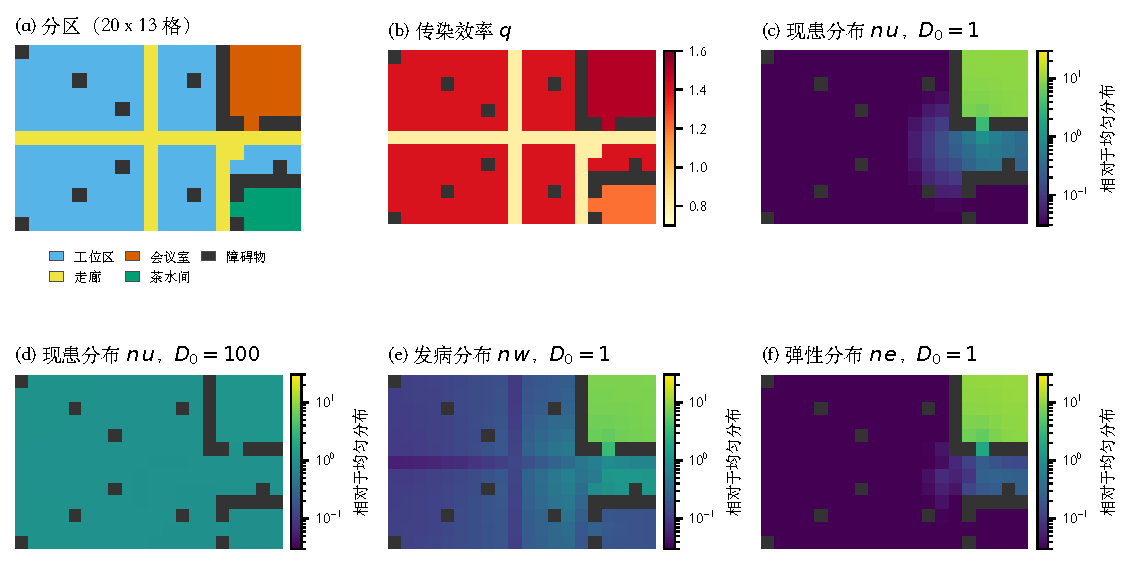
\includegraphics[width=\textwidth]{fig_hotspot_maps_zh}
  \caption{平均场模型中办公室场景的热点分布图（$\beta=0.5\perday$，
  $\gamma=0.14\perday$，同格接触核；$20\times13$ 格子中有 $\ncell=234$ 个可行走格点）。
  (a)~分区。(b)~传染效率 $q$。(c)、(d)~$\Dz=1$ 和 $\Dz=100\cellday$ 时的现患分布 $\uvec$（$\Jm$ 的右 Perron 向量）。
  (e)~发病分布 $\wvec$（$\ngm$ 的右 Perron 向量）和 (f)~弹性分布
  $e_x=\partial\ln\Rz/\partial\ln q_x$，均取 $\Dz=1\cellday$。各分布均乘以 $\ncell$，使 $1$ 对应
  均匀分布的值；色标采用对数刻度。}
  % src: data/plan_theory_sweeps.npz (office_u_D1, office_u_D100, office_w_D1, office_e_D1);
  %      drawn by code/plan_fig_theory.py
  \label{s4_geometry:fig:hotspots}
\end{figure}

图~\ref{s4_geometry:fig:hotspots} 给出办公室场景的各分布图；在该场景中，会议室（$26$ 个格点，占 234 个格点的可行走
地面的 $11.1\,\%$，$q=1.5$）只通过一条格点连边与地面的其余部分相连。在 $\Dz=1\cellday$ 时，会议室占 $\uvec$ 的
$95.9\,\%$、$\wvec$ 的 $79.2\,\%$ 和弹性的 $98.1\,\%$：$\Rz=5.107$ 实际上就是会议室的再生数，而会议室的分区下界为
$5.041$。会议室的弹性份额在 $\Dz=10$ 时降至 $20.8\,\%$，在 $\Dz=100\cellday$ 时降至 $13.4\,\%$，接近其快混合极限
$12.8\,\%$。
% src: data/plan_theory_checks.json: office/zone_counts/M, office/D0=1/area_share/M;
%      data/s4_geometry_checks.json: C_office_hotspot_identities/meeting_room_boundary_edges
% src: data/plan_theory_checks.json: office/D0=1/{prevalence_share_u,incidence_share_w,elasticity_share}/M,
%      office/D0=1/R0, office/zone_bound_meeting_room/bound
% src: data/plan_theory_checks.json: office/D0=10, office/D0=100 (elasticity_share/M);
%      limit: data/s4_geometry_checks.json: C_office_hotspot_identities/meeting_room_share_limit_e_and_w
现患分布是一个渐近对象。它需经过量级为 $1/\delta$ 的时间才能达到，而在 $\Npop$ 人中由一个指示病例引发的指数增长
阶段持续约 $\ln\Npop/\lamone$。在 $\Dz=1\cellday$ 时，$1/\delta=16$ 天，$\ln100/\lamone=7.6$ 天：在线性化动力学中，
若初始感染集中于远离会议室的某个工位格（单格初始），则在总数从初始值的 $10^2$ 倍增至 $10^4$ 倍时，其空间分布与
$\uvec$ 的全变差距离仍为 $0.996$；因此在远离热点处引入的暴发在饱和之前达不到该分布（补充材料第~\ref{S-appS_geometry:sec:hotspot}~节
中的注~\ref{S-s4_geometry:rem:transient}）。对处于这一迁移率的离散个体，平均场分布图同样不能描述感染发生在何处
（第~\ref{s6_scenes:sec:hotspot}~节）。
% src: data/plan_theory_checks.json: office/D0=1/gap, office/transient_linear/D0=1|far_workstation/tv_to_u;
% src: data/s4_geometry_checks.json: D_derived/{mixing_time_1_over_gap_days,linear_phase_ln100_over_lambda1_days}

\subsection{平均场模型中的干预措施}\label{s4_geometry:sec:examples}

补充材料第~\ref{S-appS_geometry:sec:examples}~节在办公室场景上详细计算了各项干预措施。按照定理~\ref{s3_r0:thm:edges}
的要求，走廊减速会提高 $\Rz$（走廊迁移率 $\times0.1$：$5.107\to5.222$）。隔断墙所封闭的工位间连边从
$10\pct$ 到连通性所允许的最大数目不等，在 $\Dz=1$ 时使 $\Rz$ 升高 $0.009\pct$ 至 $0.080\pct$；在三种迁移率中的任何一种下，
$80$ 次随机抽取均无一低于基线。将 $39$ 个工位格改为障碍格，移除了 $q$ 高于均值的地面：均匀混合值降低 $1.5\pct$；
$\Rz$ 在 $\Dz=1$ 时（此时它由会议室锁定）变化 $+0.065\pct$，在 $\Dz=10$ 和 $100$ 时分别变化 $-1.07\pct$ 和
$-1.49\pct$。在按弹性分布选定、并随处理进程重算分布图的一组格点上将 $q$ 减半，在 $\Dz=1$ 时比随机选格更能降低
$\Rz$（处理面积在 $5\pct$ 至 $75\pct$ 之间时，$\Rz$ 比随机选格时低 $0.35$ 至 $0.48$），但在 $\Dz=100$ 时几乎没有差别，此时定向处理
退化为处理 $q$ 最大的格点。均匀措施按精确比例缩放 $\Rz$：将 $\beta$ 乘以 $s_\beta$、每个 $q_x$ 乘以 $s_q$，使
$\Rz$ 乘以 $s_\beta s_q$。
% src: data/plan_theory_checks.json: office/corridor_multiplier_symmetric
% src: data/s4_geometry_barriers_leak.json: A_partitions/walls/*/D0=*/{change_pct,n_below_baseline}, A_partitions/barrier_cells_39_workstations
%      (wellmixed_change_pct -1.54; D0=1: +0.065; D0=10: -1.07; D0=100: -1.49)
% src: data/s4_geometry_checks.json: D_derived/targeted_ventilation/D0=1/*/gain_recomputed_vs_random (0.359, 0.352, 0.449, 0.409, 0.453, 0.482)

以上一切都属于低迁移率区间。在平均场模型中，封闭办公室在 $\Dz\gtrsim100\cellday$ 时是均匀混合的：除
命题~\ref{s3_r0:prop:expansions} 给出的修正外，$\Rz=\beta\qmean/\gamma$；定理~\ref{s4_geometry:thm:hotspots} 中的
各分布图退化为 $\stat$ 和 $\Qm\stat/\qmean$；平面布局只通过 $q$ 的面积加权均值起作用。在现实迁移率下仍然成立的是：
封闭房间中不存在尺寸效应，$\Rz$ 随 $\beta$ 和 $q$ 按比例缩放，以及停留时间形式~\eqref{s4_geometry:eq:dwell} 下的
泄漏。对离散个体，尺寸依赖性确实存在，但原因不同；这是第~\ref{s5_pair:sec}~节的主题。

% m5_pair.tex -- Main text, Section 5: discrete individuals, pair-level theory.
% Paths in "% src:" comments are relative to the repository root.
% Numbers not stored verbatim in the research directories are recomputed by code/s5_pair_checks.py
% -> data/s5_pair_checks.json (table bodies: data/s5_pair_tables.tex).  Proofs:
% Supplementary Section S4.
\section{离散个体：配对层次理论}\label{s5_pair:sec}

第~\ref{s3_r0:sec}~节的下一代矩阵计数的是传染性\emph{接触}：其列和 $\noff(x)$（式~\eqref{s3_r0:eq:offspring}）是产生于
格点 $x$ 的病例的传染率对时间积分后的期望值。在平均场模型中，每一次接触遇到的都是一个新的易感者。在
第~\ref{s2_model:sec:ibm}~节的基于个体的模型中则不然：每个人只能被感染一次，而移动缓慢的感染者会反复遇到相同的少数
几个近邻，因而之后与已感染者的接触都白白浪费了。接触的这种局部饱和是经典现象。正因为如此，具有家庭结构的流行需要
针对群体而非个体定义的再生数\citep{ball1997epidemics}；格子与网络上的配对近似所预测的入侵比质量作用下更慢
\citep{keeling1999effects}；更一般地，离散空间模型与其平均场方程有所不同\citep{durrett1994importance}。在默认参数下
（每格 0.43 人，$\Dz=1\cellday$），这一效应造成两倍之差：在办公室场景中，单独传播的指示病例平均感染 $2.27$ 人，而
$\Rz=5.11$。
% src: data/bsc_sim/02_mobility.json (D0_1.0: R1_pair_uniform_index 2.266, R0_ngm 5.107)

把感染视为两个随机游走者之间的反应并不是新思路。\citet{kenkre2014theory} 与 \citet{sugaya2018analysis} 计算了有约束与
无约束情形下一对游走者的感染概率，\citet{kenkre2021theory} 的专著对这一方法作了进一步发展。与下文最接近的是
\citet{giuggioli2022spatio}：他们在离散时间下把同处一格时的传播映射为双游走者格点游走中的一个部分吸收位点。对于初始
位置均匀随机的 $W$ 个易感游走者中的一个感染游走者，在感染期服从几何分布的情形下，他们得到二代感染的平均数等于 $W$ 乘以
传播概率的生成函数关于位置的平均（其第 6 节），称之为基本再生数，并在带反射壁的正方形区域中与模拟结果作了对照。下文定义
的 $\Ronebar$ 是该量在连续时间下的对应物。单个部分吸收位点的求解技术可追溯到 \citet{szabo1984localized}；含多个反应性缺陷
的格点表述见 \citet{giuggioli2020exact} 与 \citet{giuggioli2022spatio}，惰性异质性的类似表述见
\citet{sarvaharman2023particle}。本文新增的内容列于第~\ref{s1_intro:sec}~节。
% src: data/refs_search.json (searches; Crossref abstracts of giuggioli2022spatio and sarvaharman2023particle: reactive against inert heterogeneities)

\subsection{配对问题}\label{s5_pair:sec:pair}

本节中移动始终遵循对称规则~\eqref{s2_model:eq:hop}，因而 $\gen$ 对称且 $\pi_x=1/\ncell$；$\Npop$ 个人相互独立地从
均匀分布出发。其中一人即指示病例，在时刻 $0$ 于格点 $x$ 开始具有传染性，传染性持续时间 $\tau$ 服从速率为 $\gamma$ 的指数
分布，且与移动相互独立。考虑另外一个人，他在时刻 $0$ 位于格点 $y$。配对 $Z_t=(X_t,Y_t)$ 是 $\cells\times\cells$ 上的
马尔可夫链，其生成元为 $\mathcal{M}=\gen\otimes\Id+\Id\otimes\gen$（列指标 = 出发状态）。当配对处于状态 $(x',y')$ 时，
指示病例以式~\eqref{s2_model:eq:pairhazard} 中的速率 $h(x',y')=\beta q_{x'}P_{x'y'}/\rhobar$ 感染另一人，其中
$\rhobar=(\Npop-1)/\ncell$。

\begin{proposition}[配对感染概率]\label{s5_pair:prop:pair}
  设 $p(x,y)$ 为在其他人都不传播时，指示病例在恢复之前感染该指定的另一人的概率。记
  $\mathcal{M}=\gen\otimes\Id+\Id\otimes\gen$，并在 $\cells\times\cells$ 上记 $\mathbf{H}=\diag\,h$，则
  \begin{equation}\label{s5_pair:eq:pair}
     \one-p=\gamma\bigl(\gamma\Id+\mathbf{H}-\mathcal{M}^{\T}\bigr)^{-1}\one .
  \end{equation}
\end{proposition}

式~\eqref{s5_pair:eq:pair} 就是以速率 $\gamma+h$ 消亡的配对链的费曼–卡茨公式
$1-p(z)=\Exp_z\exp\bigl(-\int_0^{\tau}h(Z_t)\,\dd t\bigr)$：感染是双游走者过程的一个部分吸收缺陷。由于 $\gen$ 对称，
式~\eqref{s5_pair:eq:pair} 中的矩阵对称正定，该方程组可在 $\ncell^2$ 个配对状态（办公室场景为 $54{,}756$ 个）上用
共轭梯度法求解。

\begin{definition}[配对层次再生数]\label{s5_pair:def:R1}
  $\Rone(x)=(\Npop-1)\,\ncell^{-1}\sum_{y}p(x,y)$ 是产生于 $x$ 的单独传播的指示病例所致二代病例数的期望，其中其余
  $\Npop-1$ 人均为易感者、相互独立且服从均匀分布，并且只有指示病例传播；$\Ronebar=\ncell^{-1}\sum_x\Rone(x)$。配对
  层次下一代矩阵 $\ngmone$ 的元素 $(K_1)_{zx}$ 为该指示病例所感染的、\emph{被感染时位于格点 $z$} 的人数的期望；其列和
  为 $\Rone(x)$。
\end{definition}

对基于个体的模型而言，$\Rone(x)$ 是精确的：指示病例与其余每个人构成的 $\Npop-1$ 个配对同分布；它们虽然相互依赖（共享
指示病例的路径与感染期），期望仍然可以相加。当后续病例也传播时，指示病例感染的人数至多如此，因为有些人会先被他人感染。
矩阵 $\ngmone$ 可由另外 $\ncell$ 次线性求解得到；对本文的各场景，全部求解只需数秒。
% src: data/s5_pair_checks.json (saturation/*/seconds: 0.9-4.7 s for K, K1 and p)

\begin{proposition}[饱和]\label{s5_pair:prop:saturation}
  对任意场景、任意行随机接触核及任意 $\Npop\ge2$，对所有 $z,x$ 均有 $0\le(K_1)_{zx}\le K_{zx}$，且凡 $K_{zx}>0$ 处
  不等式严格成立。因此对每个 $x$ 有 $\Rone(x)<\noff(x)$，并且 $\Ronebar<\beta\langle q\rangle/\gamma$，
  $\srad(\ngmone)\le\Rz$。
\end{proposition}

由此可见，平均场矩阵计数的是暴露量，而配对层次矩阵扣除了已被感染者的暴露量。对同格接触核，定理~\ref{s3_r0:thm:bounds}
给出 $\Ronebar<\beta\langle q\rangle/\gamma\le\Rz$：均匀放置的单独传播的指示病例所感染的人数，甚至少于 $\Rz$ 的均匀混合
下界。

\subsection{均匀周期房间：闭式解}\label{s5_pair:sec:closed}

\begin{proposition}[均匀周期房间]\label{s5_pair:prop:torus}
  在 $L_1\times L_2$ 周期格子上，设向四个相邻格点中每一个的跳跃率均为 $D$，$q$ 均匀，接触核为同格接触核，并令
  $h_0=\beta q/\rhobar$。则 $p(x,y)=h_0\,g(y-x)/(1+h_0\,\gz)$，其中
  $g(r)=\int_0^\infty\e^{-\gamma t}\,\Prob(\text{相对游走在时刻 }t\text{ 位于 }0\mid\text{从 }r\text{ 出发})\,\dd t$，
  $\gz=g(0)$，且
  \begin{equation}\label{s5_pair:eq:R1}
     \Rone=\frac{\beta q/\gamma}{1+(\beta q/\rhobar)\,\gz},\qquad
     \gz=\frac1{\ncell}\sum_{k}\frac{1}{\gamma+2\mu_k},\qquad
     \mu_k=2D\,(2-\cos k_1-\cos k_2),
  \end{equation}
  其中 $k=(k_1,k_2)$ 取遍 $\tfrac{2\pi}{L_1}\{0,\dots,L_1-1\}\times\tfrac{2\pi}{L_2}\{0,\dots,L_2-1\}$。
  $\Rone$ 关于 $D$ 和 $\rhobar$ 均递增。极限：在 $\ncell$ 固定时令 $D\to\infty$，则
  $\Rone\to(\beta q/\gamma)/\bigl(1+\beta q/(\gamma(\Npop-1))\bigr)$；令 $D\to0$，则 $\Rone\to\rhobar h_0/(h_0+\gamma)$。
\end{proposition}

式~\eqref{s5_pair:eq:R1} 具有更新论证的结构。如果与该指定之人的传染性接触在其被感染之后仍继续发生，其期望次数将是
$h_0\,g(r)$，即平均场暴露量。在至少发生一次接触的条件下，配对在该时刻同处一格，接触次数的期望为 $1+h_0\gz$。两者之比
即为至少发生一次接触的概率。两个极限分别是：$\Npop$ 人均匀混合人群中的马尔可夫流行，其中每对人以速率
$\beta q/(\Npop-1)$ 相互作用；以及冻结房间，其中指示病例只感染平均 $\rhobar$ 个与其同处一格的人，每人被感染的概率为
$h_0/(h_0+\gamma)$。在四个周期格子上直接求解式~\eqref{s5_pair:eq:pair}，可再现式~\eqref{s5_pair:eq:R1}，精确到 13 位
数字。
% src: data/s5_pair_checks.json (torus: abs_err <= 7e-14); data/plan_theory_checks.json
%      (checks/torus_L5_N11: 2.316775601727); code/bsc_sim/verify/v04_finite.json (torus_L6_D1.0, torus_L8_D0.51)

\begin{corollary}[无限大地面]\label{s5_pair:cor:infinite}
  在 $\rhobar$ 固定时令 $L_1,L_2\to\infty$，则
  $\gz=\dfrac{2}{\pi}\,\dfrac{\mathcal{K}(k_*)}{\gamma+8D}$，模数为 $k_*=\dfrac{8D}{\gamma+8D}$，其中
  $\mathcal{K}$ 为第一类完全椭圆积分。特别地，对任意有限的 $D$ 有 $\Rone<\beta q/\gamma$：对大房间，这一修正并不消失。
\end{corollary}

当 $8D\gg\gamma$ 时，由 $\mathcal{K}$ 的对数奇异性得 $\gz\approx\ln(64D/\gamma)/(8\pi D)$：修正随迁移率只按
$\ln D/D$ 衰减，这反映了平面游走的常返性。

\begin{observation}[反射壁]\label{s5_pair:obs:reflecting}
  对带反射壁的矩形房间，在式~\eqref{s5_pair:eq:R1} 中取
  $\mu_k=2D(2-\cos(k_1\pi/L_1)-\cos(k_2\pi/L_2))$，$k_i=0,\dots,L_i-1$（即按格点平均的 $\gz$），所得结果再现由精确配对
  求解~\eqref{s5_pair:eq:pair} 得到的 $\Ronebar$，在 $L=4,\dots,28$ 与 $D=0.51,1,10$ 下误差在 $0.9\,\%$ 以内
  （最大偏差出现在 $D=0.51$、$L=7$）。
\end{observation}
% src: data/bsc_sim/02_finite_size.json (pair_closed_form, pair_exact);
%      data/s5_pair_checks.json (finite_size: max 0.90 % at D0.51_L7; by D: 0.90 %, 0.46 %, 0.02 %)

\subsection{有限尺寸效应的形式}\label{s5_pair:sec:finite}

对平均场模型而言，封闭房间不存在尺寸效应（定理~\ref{s4_geometry:thm:closed}）。离散的人确实表现出尺寸效应，其形式
正是式~\eqref{s5_pair:eq:R1}。图~\ref{s5_pair:fig:finite}（数值见补充材料表~\ref{S-s5_pair:tab:finite}）在均匀
$L\times L$ 房间中比较了平均场再生数、闭式解、精确配对求解与模拟，每格有 $0.381$ 个其他人（即无障碍物的 $20\times13$
格子的 260 个格点上有 99 人；办公室场景有 234 个可行走格点，该值为 $0.423$）。
% src: data/bsc_sim/02_finite_size.json (rho_bar = 99/260); data/s2_model_scenes.json -> scenes.office.rho_bar (0.4231)

\begin{figure}[tbp]
\centering
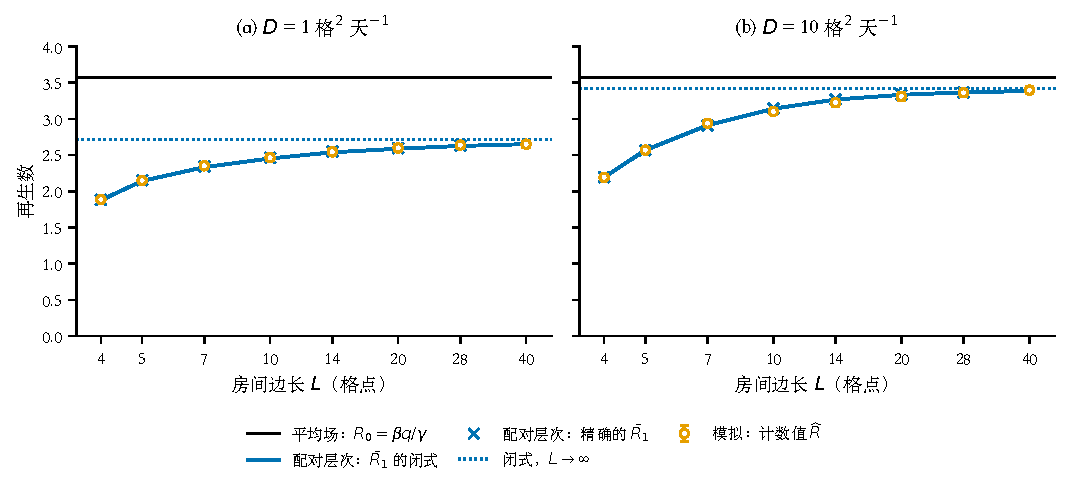
\includegraphics[width=\textwidth]{fig5_1_finite_size_zh}
\caption{离散个体的有限尺寸效应。带反射壁的均匀 $L\times L$ 房间，$q=1$，同格接触核，$\rhobar\approx0.381$（每格其他
人数；$L=4$ 时 $\Npop=7$，至 $L=40$ 时为 $610$），迁移率 (a) $D=1$，(b) $D=10\cellday$。黑线：平均场
$\Rz=\beta q/\gamma=3.571$。蓝线：采用反射壁谱的闭式解~\eqref{s5_pair:eq:R1}；叉号：精确配对求解~\eqref{s5_pair:eq:pair}
（$L\le28$）；点线：无限格子（推论~\ref{s5_pair:cor:infinite}）。圆点：只有指示病例传播时，均匀放置的指示病例的二代病例
计数值 $\Rhat$，每个点 20{,}000 次模拟，误差棒为 95\pct{} 置信区间。}
\label{s5_pair:fig:finite}
% src: data/bsc_sim/02_finite_size.json; figure script code/fig_finite_size.py
\end{figure}

在 $D=1$ 时，单独传播的指示病例在有 7 人的 $4\times4$ 房间中平均感染 $1.88$ 人，在有 153 人的 $20\times20$ 房间中平均
感染 $2.60$ 人，在相同占据率的无限大地面上平均感染 $2.71$ 人；而平均场模型在任意尺寸下均为 $3.57$。修正项是一个格子
格林函数。它随迁移率增大而减小：在 $L=10$ 时，计数值从 $D=1$ 时的 $2.46$ 升至 $D=10$ 时的 $3.10$。并且它在
$L\to\infty$ 时并不消失：无限大地面上的值在 $D=1$ 时为 $\beta q/\gamma$ 的 $76\,\%$，在 $D=10$ 时为 $96\,\%$。原因在于
反复遇到相同的人：在小房间中是因为人少，在大地面上是因为缓慢的平面游走者会回到其近邻身边；并没有任何东西从墙壁泄漏
出去。在所扫描的 24 个房间中，闭式解在 23 个房间落在计数值的 95\,\% 区间内；精确求解在已计算的 21 个房间中有 19 个
落在该区间内；第二模拟器在重新运行的七个房间（包括上述两个例外）中与精确求解相差均在 $1.7$ 个标准误以内。
% src: data/bsc_sim/02_finite_size.json; data/s5_pair_checks.json
%      (finite_size/ratio_to_meanfield: D1.0_Linf 0.759, D10.0_Linf 0.958; closed_outside_sim_ci, exact_outside_sim_ci;
%      finite_size_check: z between -1.35 and 1.65); code/bsc_sim/verify/v04_finite.json

\subsection{迁移率：两个层次上的相反趋势}\label{s5_pair:sec:mobility}

\begin{figure}[tbp]
\centering
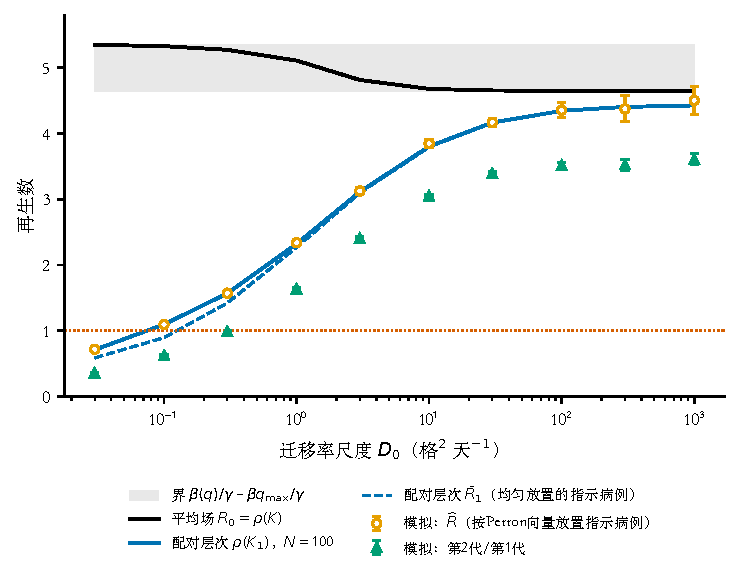
\includegraphics[width=0.72\textwidth]{fig5_5_R_vs_mobility_zh}
\caption{办公室场景的各再生数随迁移率尺度 $\Dz$ 的变化（$\Npop=100$，同格接触核，$\beta=0.5\perday$，
$\gamma=0.14\perday$）。黑线：平均场 $\Rz=\srad(\ngm)$；灰色带：其上下界 $\beta\langle q\rangle/\gamma=4.643$ 与
$\beta\qmax/\gamma=5.357$。蓝色实线：配对层次下一代矩阵的谱半径 $\srad(\ngmone)$；蓝色虚线：对均匀放置的指示病例取平均的
$\Ronebar$，它在 $\Dz$ 较小时更低。圆点：只有指示病例传播时，产生位置按 $\ngmone$ 的 Perron 向量分布的指示病例的二代
病例计数值 $\Rhat$。三角：指示病例及其直接感染的病例都传播时，第二代病例数除以第一代病例数。误差棒为 95\pct{} 置信区间；
模拟次数与数值见补充材料表~\ref{S-s5_pair:tab:mobility}。点线标出数值 1。}
\label{s5_pair:fig:mobility}
% src: data/bsc_sim/02_mobility.json; figure script code/bsc_sim/experiments/21_figures_more.py
\end{figure}

办公室场景的平均场 $\Rz$ 随迁移率减小（定理~\ref{s3_r0:thm:mobility}），从 $\Dz=0.03$ 时的 $5.35$ 降至 $\Dz=1000$ 时的
$4.64$；配对层次的各数则增大，$\Ronebar$ 从 $0.59$ 增至 $4.42$：移动更快的指示病例会遇到更多不同的人
（图~\ref{s5_pair:fig:mobility}）。在 $\Dz=1$ 时，$\Ronebar=2.27$ 为 $\Rz=5.11$ 的 $44\,\%$；在 $\Dz=10$ 时为 $81\,\%$，
在 $\Dz=100$ 时为 $93\,\%$。在 $\Dz=1000$ 时，$\Ronebar=4.425$ 接近
$(\beta\langle q\rangle/\gamma)/\bigl(1+\beta\langle q\rangle/(\gamma(\Npop-1))\bigr)=4.435$，即 100 人均匀混合人群的值
（参见命题~\ref{s5_pair:prop:torus} 中 $D\to\infty$ 的极限）。计数得到的二代病例数与之相符：400{,}000、400{,}000 和
100{,}000 次模拟的样本在 $\Dz=1$、$10$ 和 $100$ 时分别给出 $2.265\pm0.004$、$3.793\pm0.006$ 和 $4.340\pm0.015$，而
$\Ronebar=2.266$、$3.793$ 和 $4.341$。
% src: data/bsc_sim/02_mobility.json; data/s5_pair_checks.json (mobility: R1bar_over_R0
%      0.444, 0.811, 0.934; office_wellmixed_finite_population 4.4349)
% src: data/s5_pair_large_sample.json (office|D0=1: mean 2.2648, se 0.0039; office|D0=10: 3.7930, 0.0064; office|D0=100: 4.3399, 0.0145)
在 $\rhobar=0.381$、$\beta q=0.5\perday$ 的无限均匀格子上，比值 $\Rone/\Rz$ 在 $D=0.24$ 时为 $0.5$，在 $D=3.5$ 时为
$0.9$，在 $D=52\cellday$ 时为 $0.99$（补充材料图~\ref{S-s5_pair:fig:validity}）。因此，当许多人共享同一接触邻域，或者
人们在一个感染期内移动得足够远、能遇到新的人时，平均场再生数是适用的；$\Dz=1$ 的各场景两个条件都不满足。在
$\Dz\approx2.4\times10^3\cellday$（第~\ref{s2_model:sec:regime}~节）时，无限格子上的比值为 $0.9997$，有限房间中剩下的
只是均匀混合的有限人群因子。
% src: data/s5_pair_checks.json (infinite: D_for_ratio_*; D=2400 ratio 0.99970)

\subsection{后续世代：不是阈值}\label{s5_pair:sec:threshold}

配对层次对第一代是精确的，但也仅止于第一代。二代病例的处境不同于单独传播的指示病例：它从其传染者所在格点或相邻格点开始，而
传染者不能再被感染；它也靠近其传染者已造成的其他病例，因此其邻域中已有一部分被用尽。在 $\Dz=1$ 的办公室中，第二代是
第一代的 $1.63$ 倍（$1.61$--$1.65$），而 $\srad(\ngmone)=2.32$。这两个数之比在 $\Dz=0.03$ 时为 $0.50$，在 $\Dz=1$ 时为
$0.70$，在 $\Dz\ge10$ 时为 $0.80$--$0.81$；最后这个值就是 100 人均匀混合人群的值，其中指示病例与其直接感染的病例争夺
相同的易感者（用相同设计的均匀混合模型做 $200{,}000$ 次模拟，得 $0.81$）。
% src: data/bsc_sim/02_mobility.json (sim_gen2_over_gen1, R1_pair_ngm); data/s5_pair_checks.json
%      (mobility: gen_ratio_over_rhoK1; wellmixed_generation_ratio: 3.589 / 4.435 = 0.809)

\begin{remark}[$\Rone$ 与 $\srad(\ngmone)$ 不是阈值量]\label{s5_pair:rem:threshold}
无论 $\Ronebar>1$ 还是 $\srad(\ngmone)>1$，都不意味着可能发生大规模暴发。在采用同格接触核、$\Dz=1$ 的地铁车厢中
（$270$ 个格点上 $310$ 人；按格点取中位数，乘客两次跳跃之间需等待 48 天），$\srad(\ngmone)=2.24$，$\Ronebar=1.51$，
单独传播的指示病例的二代病例计数值为 $1.52$（$1.49$--$1.54$；20{,}000 次模拟）。然而第二代为第一代的 $0.61$ 倍；
在一个模拟器的 2{,}000 次模拟和另一个模拟器的 3{,}000 次模拟中，没有一次暴发波及 $10\pct$ 的乘客（平均罹患率 $1.1\pct$）：
指示病例感染的是与其同格的人，而这些人已无人可感染。同一情形下的平均场值为 $\Rz=9.84$。因此，不能以“$\Rone<1$”来评判
干预措施，也不应把 $\srad(\ngmone)$ 理解为离散系统的基本再生数。格点随机游走者之间的感染存在阈值，这一点是已知的：
对 $\mathbb{Z}^d$ 上带恢复与再感染的独立游走者有严格结果\citep{kesten2006phase}，对扩散流行过程（包括其具有永久免疫的
变体）有模拟结果\citep{maia2007diffusive,carvalho2025generalized}。这些结果针对的是无限或大型的均匀格子，不能为本文所
考虑的小型异质房间给出可计算的阈值。本文没有任何量能够预测低迁移率下基于个体的模型的阈值或最终规模；这些量在
第~\ref{s6_scenes:sec}~节中通过模拟得到。
\end{remark}
% src: data/bsc_sim/03_scenes.json (metro|D0=1|samecell: R1_pair_ngm 2.2437, R1_pair_uniform_index 1.5138,
%      R0_ngm 9.836, n_major 0 of 2000, attack_all_mean 0.0112, gen2_over_gen1 0.608);
%      code/bsc_sim/verify/v05_scenes.json (metro|1.0|same: 0 of 3000, gen2_over_gen1 0.609);
%      data/bsc_sim/01_validation.json (D_pair_theory, metro same cell: 1.517, 1.495-1.539);
%      data/s5_pair_checks.json (saturation/metro: rho_K1 2.2437, R1bar 1.5138, median_cell_time_between_hops_days 48.5)

总之，在低迁移率下，离散个体之间一次暴发的最初几步由三个数刻画，必须将它们区分开来：平均场 $\Rz$，它计数暴露量，其矩阵
从上方界定配对层次的矩阵（命题~\ref{s5_pair:prop:saturation}）；配对层次的 $\Rone(x)$，它是单独传播的指示病例所感染
人数的精确期望；以及从一代到下一代的增长，它还要更低，而我们没有它的公式。

% m6_simulation.tex -- Main text, Section 6: exact stochastic simulation of four indoor scenes and of interventions.
% Paths in "% src:" comments are relative to the repository root.
% Table bodies between "% BEGIN AUTO" and "% END AUTO" are written by code/s6_scenes_tables.py
% (-> data/s6_scenes_tables.tex) and pasted by code/s6_scenes_paste_tables.py; every
% derived number quoted in the prose is stored in data/s6_scenes_numbers.json (key given in the comment).
% Details, further tables and figures: Supplementary Section S5.
% Chinese edition: the numbers of the table body are copied unchanged; only the words are translated.
\section{四个室内场景的精确随机模拟}\label{s6_scenes:sec}

第~\ref{s3_r0:sec}--\ref{s5_pair:sec}~节给出了两种无需模拟即可计算的再生数：平均场 $\Rz$ 与配对层次的 $\Ronebar$。
本节报告：第~\ref{s2_model:sec:ibm}~节的基于个体的模型在表~\ref{s2_model:tab:scenes} 所列四个场景中表现如何、这两个数各自
能在多大程度上描述它，以及模型对干预措施说明了什么。全部结果均针对 $\Dz=1$、$10$ 和 $100\cellday$ 给出，这三个值都
远低于步行迁移率（第~\ref{s2_model:sec:regime}~节）；下文报告的对平均场理论的偏离在 $\Dz=1$ 时很大，在 $\Dz=100$ 时
很小。

\subsection{模拟器与模拟方案}\label{s6_scenes:sec:protocol}

对基于个体的模型逐事件进行精确模拟（补充材料图~\ref{S-appA_numerics:fig:algorithm}）；二代病例数在记录下来的感染树上
计数。每个重复样本使用 xoshiro256** 发生器\citep{blackman2021scrambled}的一条专属随机数流。该模拟器与以下各项在
分布上一致：另行编写的纯 Python 实现、单格模型的精确最终规模分布、（通过暴露恒等式）下一代矩阵，以及高占据率和高
迁移率下的平均场方程（补充材料表~\ref{S-appA_numerics:tab:simulator}）。此外，$\Dz=1$ 时的场景结果以及 $\Dz=10$ 时的
大部分结果，还用第二模拟器重新运行；两者在蒙特卡罗误差范围内一致，两处最大的差异分别为 $1.6$ 和 $2.1$ 个标准误
（补充材料第~\ref{S-appS_sim:sec:scenes}~节）。
% src: code/bsc_sim/verify/v05_scenes.json (p_major, n); data/s6_scenes_numbers.json: check_scenes.*.z_first_minus_check (1.56, 2.11)

人员从平稳（均匀）分布出发，其中一人在时刻 $0$ 具有传染性，因而其所在格点服从均匀分布。对每种场景、迁移率与接触核的
组合，各模拟 2{,}000 次流行过程，直至不再有感染者为止。\emph{罹患率}是 $\Npop$ 人中曾被感染者所占的比例，包括指示病例在内。
若一次暴发的罹患率不低于 $10\,\%$，则称之为\emph{大规模}暴发；$P_{\mathrm{maj}}$ 为大规模暴发所占的比例，并给出
Wilson $95\,\%$ 区间；该阈值是一种约定，其影响在补充材料第~\ref{S-s6_scenes:sec:pmajor}~节中加以量化。二代病例的计数值
$\Rhat$ 是另外 2{,}000 次只有指示病例传播的模拟的均值。平均场对应量为 $\Rz$、式~\eqref{s2_model:eq:meanfield} 的解，以及
分支过程的暴发概率 $P_{\mathrm{br}}$；在该分支过程中，病例以生成元 $\gen$ 游走，以速率 $\gamma$ 恢复，并在位于格点 $x$
时以速率 $\beta q_x$ 产生新病例，每个新病例以概率 $P_{xy}$ 置于格点 $y$；其各传播链的灭绝概率 $s_x$ 是下述方程组的最小
非负解\citep{andersson2000stochastic}：
\begin{equation}\label{s6_scenes:eq:branching}
  \gamma\,(1-s_x)+\beta q_x\,s_x\Bigl(\sum_{y}P_{xy}s_y-1\Bigr)+\sum_{y}\hop{x}{y}\,(s_y-s_x)=0 ,
  \qquad P_{\mathrm{br}}=1-\frac1{\ncell}\sum_{x\in\cells}s_x
\end{equation}
% src: code/bsc_sim/experiments/03_scenes.py (n_rep = 2000, T_MAX = 400 d); code/bsc_sim/src/bsc_sim/theory.py (extinction_probability, meanfield_ode)

\subsection{四个场景中的结局}\label{s6_scenes:sec:outcomes}

\begin{table}[tbp]
\centering
\caption{四个场景的精确模拟结果与平均场理论结果。迁移率尺度为 $\Dz$（\cdunit），$\beta=0.5\perday$，
$\gamma=0.14\perday$，频率依赖发生率；每行 2{,}000 次流行过程，一个均匀放置的指示病例，封闭房间。$\Rz$：平均场基本
再生数。$\Ronebar$：配对层次上均匀放置的指示病例的二代病例期望数（定义~\ref{s5_pair:def:R1}）。$\Rhat\pm$SE：二代
病例数的计数均值，仅指示病例传播（另外 2{,}000 次模拟）。$P_{\mathrm{maj}}$：罹患率不低于 $10\,\%$ 的模拟所占比例
（Wilson 区间）。$P_{\mathrm{br}}$：平均场分支过程值~\eqref{s6_scenes:eq:branching}。罹患率：分别对大规模暴发和对全部
模拟取平均。峰值：对大规模暴发取平均的最大感染比例（0.5 天网格）及其出现日。ODE：从均匀分布的一名感染者出发时平均场
方程给出的罹患率（\%）/ 峰值感染比例（\%）/ 峰值时间，以及一名感染者位于单个格点时的峰值感染比例（\%）/ 峰值时间
（对初始格点取平均；仅 1\,m 接触核）。短横线表示没有发生大规模暴发。}
\label{s6_scenes:tab:scenes}
% src: data/bsc_sim/03_scenes.json (all columns but the last); data/s6_scenes_ode_pointseed.json (last column)
\footnotesize
\setlength{\tabcolsep}{2.7pt}
\begin{tabular}{@{}rccccccccccc@{}}
\toprule
 & & & & & & \multicolumn{2}{c}{罹患率（\%）} & \multicolumn{2}{c}{峰值} & \multicolumn{2}{c}{平均场 ODE}\\
\cmidrule(lr){7-8}\cmidrule(lr){9-10}\cmidrule(l){11-12}
$\Dz$ & $\Rz$ & $\Ronebar$ & $\Rhat\pm{}$SE & $P_{\mathrm{maj}}$（95\,\% 置信区间） & $P_{\mathrm{br}}$ & 大规模 & 全部 &
\% & 天 & 均匀初始 & 单格初始\\
\midrule
% BEGIN AUTO s6_scenes:tab:scenes (numbers copied unchanged from ../sections/m6_simulation.tex)
\multicolumn{12}{@{}l}{\emph{办公室}，$\Npop=100$，$\ncell=234$，1\,m 接触核（与同格接触核相同）；$\beta\langle q\rangle/\gamma=4.64$，$\beta\qmax/\gamma=5.36$}\\
1 & 5.11 & 2.27 & 2.26\,$\pm$\,0.06 & 0.496 (0.474--0.518) & 0.781 & 44.3 & 23.2 & 12.7 & 23.2 & 98.9 / 45.1 / 11.5 & 32.8 / 20.4\\
10 & 4.68 & 3.79 & 3.90\,$\pm$\,0.09 & 0.762 (0.743--0.781) & 0.783 & 96.3 & 73.8 & 39.0 & 16.5 & 99.0 / 45.7 / 11.5 & 44.1 / 12.8\\
100 & 4.65 & 4.34 & 4.11\,$\pm$\,0.10 & 0.770 (0.751--0.788) & 0.784 & 98.8 & 76.4 & 48.4 & 12.6 & 99.0 / 45.9 / 11.5 & 45.9 / 11.6\\
\addlinespace
\multicolumn{12}{@{}l}{\emph{超市}，$\Npop=150$，$\ncell=278$，1\,m 接触核（与同格接触核相同）；$\beta\langle q\rangle/\gamma=3.26$，$\beta\qmax/\gamma=7.14$}\\
1 & 4.39 & 1.99 & 1.97\,$\pm$\,0.05 & 0.436 (0.414--0.458) & 0.667 & 42.0 & 19.4 & 10.1 & 31.5 & 93.6 / 28.9 / 17.0 & 23.7 / 25.7\\
10 & 3.39 & 2.86 & 2.86\,$\pm$\,0.07 & 0.648 (0.627--0.669) & 0.685 & 92.1 & 60.0 & 30.6 & 22.6 & 95.4 / 33.4 / 17.5 & 33.1 / 18.0\\
100 & 3.28 & 3.15 & 3.04\,$\pm$\,0.08 & 0.686 (0.665--0.706) & 0.692 & 95.3 & 65.7 & 36.1 & 19.3 & 95.7 / 33.7 / 18.5 & 33.7 / 18.3\\
\addlinespace
\multicolumn{12}{@{}l}{\emph{教室}，$\Npop=80$，$\ncell=148$，1\,m 接触核（平均 4.6 个格点）；$\beta\langle q\rangle/\gamma=4.71$，$\beta\qmax/\gamma=7.14$}\\
1 & 5.87 & 2.58 & 2.62\,$\pm$\,0.06 & 0.614 (0.592--0.635) & 0.767 & 39.2 & 25.2 & 14.1 & 16.3 & 98.4 / 42.6 / 11.0 & 31.7 / 18.1\\
10 & 4.93 & 3.72 & 3.72\,$\pm$\,0.09 & 0.750 (0.731--0.768) & 0.777 & 94.0 & 70.9 & 35.0 & 17.3 & 98.8 / 45.0 / 10.5 & 41.3 / 12.8\\
100 & 4.73 & 4.32 & 4.30\,$\pm$\,0.10 & 0.779 (0.760--0.797) & 0.785 & 98.6 & 77.2 & 48.8 & 12.2 & 99.1 / 46.5 / 11.0 & 46.5 / 11.0\\
\addlinespace
\multicolumn{12}{@{}l}{\emph{教室}，$\Npop=80$，$\ncell=148$，同格接触核；$\beta\langle q\rangle/\gamma=4.71$，$\beta\qmax/\gamma=7.14$}\\
1 & 6.18 & 1.56 & 1.53\,$\pm$\,0.04 & 0.276 (0.256--0.295) & 0.766 & 19.7 & 7.6 & 8.5 & 15.2 & 98.0 / 40.0 / 11.0 & \\
10 & 4.96 & 3.20 & 3.15\,$\pm$\,0.07 & 0.695 (0.674--0.715) & 0.777 & 89.1 & 62.5 & 29.7 & 20.7 & 98.8 / 44.5 / 10.5 & \\
100 & 4.73 & 4.23 & 4.39\,$\pm$\,0.10 & 0.771 (0.753--0.789) & 0.785 & 98.6 & 76.4 & 48.2 & 12.3 & 99.1 / 46.5 / 11.0 & \\
\addlinespace
\multicolumn{12}{@{}l}{\emph{地铁车厢}，$\Npop=310$，$\ncell=270$，1\,m 接触核（平均 11.1 个格点）；$\beta\langle q\rangle/\gamma=9.06$，$\beta\qmax/\gamma=10.00$}\\
1 & 9.24 & 5.58 & 5.59\,$\pm$\,0.10 & 0.879 (0.864--0.893) & 0.888 & 93.7 & 82.4 & 24.9 & 21.9 & 100.0 / 64.1 / 7.0 & 35.0 / 16.3\\
10 & 9.16 & 6.32 & 6.44\,$\pm$\,0.13 & 0.878 (0.863--0.892) & 0.888 & 98.4 & 86.5 & 27.5 & 21.0 & 100.0 / 64.3 / 7.0 & 36.3 / 15.7\\
100 & 9.08 & 7.54 & 7.58\,$\pm$\,0.16 & 0.891 (0.877--0.904) & 0.889 & 99.9 & 89.0 & 35.3 & 16.5 & 100.0 / 64.6 / 7.0 & 42.2 / 13.8\\
\addlinespace
\multicolumn{12}{@{}l}{\emph{地铁车厢}，$\Npop=310$，$\ncell=270$，同格接触核；$\beta\langle q\rangle/\gamma=9.06$，$\beta\qmax/\gamma=10.00$}\\
1 & 9.84 & 1.51 & 1.56\,$\pm$\,0.04 & 0.000 (0.000--0.002) & 0.888 & -- & 1.1 & -- & -- & 100.0 / 61.4 / 7.0 & \\
10 & 9.31 & 3.00 & 3.05\,$\pm$\,0.07 & 0.349 (0.329--0.371) & 0.888 & 17.3 & 7.7 & 5.0 & 23.4 & 100.0 / 62.9 / 7.0 & \\
100 & 9.09 & 6.10 & 6.24\,$\pm$\,0.14 & 0.858 (0.842--0.873) & 0.889 & 98.6 & 84.7 & 24.0 & 24.4 & 100.0 / 64.4 / 7.0 & \\
% END AUTO s6_scenes:tab:scenes
\bottomrule
\end{tabular}
\end{table}

\paragraph{二代病例。}配对层次的 $\Ronebar$ 在表~\ref{s6_scenes:tab:scenes} 的全部 18 行中都再现了计数值 $\Rhat$：最大
偏差为 $2.3$ 个标准误（办公室，$\Dz=100$），其余各行均不超过 $2$ 个标准误。平均场 $\Rz$ 则不能再现：$\Dz=1$ 时，在
办公室、超市、教室和地铁车厢中，比值 $\Rhat/\Rz$ 分别为 $0.44$、$0.45$、$0.45$ 和 $0.60$，$\Dz=100$ 时升至
$0.84$--$0.93$。后续世代的增长还要更慢：在 $\Dz=1$ 的完整流行中，第二代病例数分别是第一代的 $1.29$、$1.38$、$1.32$ 和
$1.84$ 倍（第二模拟器：$1.39$、$1.40$、$1.29$、$1.87$），而 $\srad(\ngmone)=2.32$、$2.20$、$2.83$ 和 $5.72$。
% src: data/s6_scenes_numbers.json: Rhat_vs_R1bar (largest_abs_z = 2.28, n_rows_abs_z_gt_2 = 1)
% src: data/bsc_sim/03_scenes.json (R_index_alone_mean, R0_ngm); s6_scenes_numbers.json: scenes.*.Rhat_over_R0
% src: data/bsc_sim/03_scenes.json: gen2_over_gen1, R1_pair_ngm (rows D0 = 1, range1m);
%      code/bsc_sim/verify/v05_scenes.json: gen2_over_gen1 (1.388, 1.397, 1.291, 1.869)

\paragraph{低迁移率，$\Dz=1$。}在办公室、超市和教室中，平均场描述对每一项整体流行结局都失效。在办公室中，
$P_{\mathrm{maj}}=0.496$（$0.474$--$0.518$），而 $P_{\mathrm{br}}=0.781$；大规模暴发感染 $44.3\,\%$ 的人（均值的
$95\,\%$ 区间为 $42.9$--$45.6\,\%$），而平均场方程给出 $98.9\,\%$；其感染比例在第 $23.2$ 天达到峰值 $12.7\,\%$，而平均场
方程从均匀初始出发给出第 $11.5$ 天的 $45.1\,\%$，从单个格点出发给出第 $20.4$ 天的 $32.8\,\%$。罹患率分布不呈双峰：全部
模拟中分别有 $27\,\%$、$28\,\%$ 和 $43\,\%$ 以介于 $10\,\%$ 与 $50\,\%$ 之间的罹患率结束，而 $\Dz=10$ 时这一比例至多为
$0.6\,\%$。传播是局部而缓慢的，暴发可在任何规模上停滞。地铁车厢的乘客虽然几乎不移动，结果却更接近其平均场
（$P_{\mathrm{maj}}=0.879$，对比 $0.888$），因为车厢内每格有 $1.15$ 人，且 1\,m 接触核平均覆盖 $11.1$ 个格点，因此一名
感染者的接触范围内约有 $13$ 人。
% src: data/bsc_sim/03_scenes.json: "office|D0=1|range1m" (p_major, p_major_lo/hi, p_major_branching,
%      attack_major_mean/lo/hi (0.4427, 0.4289, 0.4565), ode_attack, peak_prev_major_mean, peak_time_major_mean, ode_peak_prev, ode_peak_time);
%      data/s6_scenes_ode_pointseed.json: "office|D0=1|range1m".point_seed
% src: s6_scenes_numbers.json: summary_by_D0."D0=1".frac_runs_attack_10_to_50pct (0.2715, 0.2765, 0.4285);
%      summary_by_D0."D0=10".frac_runs_attack_10_to_50pct (max 0.006)
% src: 03_scenes.json: "metro|D0=1|range1m" (p_major, p_major_branching, occupancy = 1.148, kernel_cells = 11.13; 1.148 x 11.13 = 12.8)

\paragraph{较高迁移率，$\Dz\ge10$。}采用 1\,m 接触核时，平均场对暴发概率和罹患率是适用的：$\Dz=10$ 时
$P_{\mathrm{br}}$ 比 $P_{\mathrm{maj}}$ 高 $0.01$--$0.04$，$\Dz=100$ 时至多高 $0.014$；大规模暴发的罹患率在 $\Dz=10$ 时
比平均场值低 $1.5$--$4.9$ 个百分点，在 $\Dz=100$ 时与之相差不超过 $0.5$ 个百分点。峰值高度与峰值时间则是另一回事：
$\Dz=10$ 时，即使平均场方程从单个格点出发，模拟所得的峰值仍更低，且推迟约四到五天。
% src: data/s6_scenes_numbers.json: summary_by_D0."D0=10" (branch_minus_sim 0.0096..0.0368; ode_minus_sim_attack_points 1.54..4.87),
%      summary_by_D0."D0=100" (branch_minus_sim -0.0023..0.0143; ode_minus_sim_attack_points 0.10..0.48); four 1 m-kernel rows

\paragraph{暴发概率。}由一个病例引发的传播链的早期灭绝在每个场景中都会发生。指示病例的二代病例数是过度离散的，方差为
均值的 $2.6$ 至 $5.0$ 倍，且有 $10\,\%$ 至 $31\,\%$ 的指示病例没有感染任何人；过度离散会降低暴发概率
\citep{lloydsmith2005superspreading}；以模拟所得的后代分布为输入的 Galton--Watson 过程，在罹患率分布呈双峰的各处都能把
$P_{\mathrm{maj}}$ 再现到 $0.011$ 以内（补充材料表~\ref{S-s6_scenes:tab:pmajor}）。
% src: data/bsc_sim/03b_outbreak_probability.json: var_over_mean (2.598..5.022), p_zero (0.104..0.310);
%      s6_scenes_numbers.json: pmajor_ranges.gw_minus_sim_other_rows_max_abs = 0.0105

\paragraph{接触核}是一种建模选择；当格点小于接触范围时，它的后果很大。采用同格接触核时，地铁车厢（格点边长 $0.5$\,m）
在 $\Dz=1$ 时不产生暴发：2{,}000 次模拟中没有一次达到 $10\,\%$ 的罹患率（第二模拟器的 3{,}000 次中也没有），尽管
$\Rz=9.84$，$\Ronebar=1.51$，$\srad(\ngmone)=2.24$（注~\ref{s5_pair:rem:threshold}）。采用 1\,m 接触核时，同一车厢是暴发
性最强的场景（$P_{\mathrm{maj}}=0.879$）。本文所计算的任何量都不能预测低迁移率下离散系统的阈值；它必须通过模拟得到。
% src: 03_scenes.json: "metro|D0=1|samecell" (n_major = 0, R0_ngm = 9.836, R1_pair_uniform_index = 1.514, R1_pair_ngm = 2.244);
%      code/bsc_sim/verify/v05_scenes.json: "metro|1.0|same" (n = 3000, p_major = 0)

\subsection{感染发生在何处}\label{s6_scenes:sec:hotspot}

对均匀放置的指示病例，第 $g$ 代病例被感染时所在格点的分布，在平均场模型中与 $\ngm^{g}\one$ 成正比，在配对层次描述中
与 $\ngmone^{g}\one$ 成正比。在 $\Dz=1$ 的办公室中，平均场分布图与模拟所得分布图在第一代不相关，在随后两代呈负相关
（$r=0.09$、$-0.23$、$-0.37$；40{,}000 次暴发），而配对层次分布图给出 $r=0.88$、$0.82$、$0.71$（补充材料
表~\ref{S-s6_scenes:tab:hotspot} 与图~\ref{S-s6_scenes:fig:spatial}）。最热的格点是邻接走廊的工位格，而不是主导
第~\ref{s4_geometry:sec:hotspots}~节平均场分布图的会议室：到第三代时，会议室的感染率从平均水平降至 $0.68$，而平均场预测
为 $1.44$，这与局部耗竭相符。因此，“感染集中于会议室”这样的表述是一种平均场表述；对低迁移率下的离散个体，分布图必须
取自 $\ngmone$ 或模拟。
% src: data/bsc_sim/04_spatial.json: "office|D0=1".gen1..3 (r_meanfield 0.092, -0.235, -0.371; r_pair 0.875, 0.816, 0.709)
% src: data/s6_scenes_numbers.json: office_cell_classes."D0=1".classes.M.sim (0.998, 0.877, 0.677), .meanfield (1.154, 1.295, 1.436)

\subsection{干预措施}\label{s6_scenes:sec:interventions}

配对风险率~\eqref{s2_model:eq:pairhazard} 采用两种标定。在\emph{频率依赖}（FD）标定下，$\rhobar=(\Npop-1)/\ncell$ 按
当前房间计算，因此无论房间多么拥挤，位于格点 $x$ 的感染者都以速率 $\beta q_x$ 产生传染性接触。在\emph{密度依赖}（DD）
标定下，$\rhobar$ 固定为某一基线房间的取值 $\rhobar_{\mathrm{ref}}$，因此每对人的风险率固定，接触速率随拥挤程度增加。
在平均场中，
\begin{equation}\label{s7_interventions:eq:dd}
  \Rz^{\mathrm{DD}}=\frac{\rhobar}{\rhobar_{\mathrm{ref}}}\,\Rz^{\mathrm{FD}},\qquad
  \rhobar=\frac{\Npop-1}{\ncell}.
\end{equation}
哪一种传播律能描述室内的人群是一个经验问题\citep{mccallum2001should,begon2002clarification}，模型本身无法判定；下文的
每个结果都注明所用的是哪一种。细节见补充材料第~\ref{S-appS_sim:sec}~节。

\paragraph{分区隔离。}在一个两区房间中（$20\times13$ 格点，工作区占地面 70\,\%，迁移率为 $0.3\,\Dz$；中央走廊带占
30\,\%，迁移率为 $2\,\Dz$），对比度 $c$ 在面积平均 $\langle q\rangle=1.2$ 固定的条件下重新分配 $q$：
\begin{equation}\label{s7_interventions:eq:contrast}
  q_{\mathrm C}=1.2\,(1-c),\qquad q_{\mathrm W}=1.2\,\bigl(1+\tfrac37c\bigr).
\end{equation}
由定理~\ref{s3_r0:thm:bounds}，只要 $c\ne0$，就有 $\Rz>\beta\langle q\rangle/\gamma=4.286$；在 $c=0.583$
（$q_{\mathrm W}=1.5$，$q_{\mathrm C}=0.5$）时，$\Dz=1$ 下 $\Rz=4.972$，比均匀房间高 16\,\%。对于 $\Dz=1$、$\Npop=100$ 的
离散个体，开启对比度后，所计数的一切都\emph{下降}（补充材料图~\ref{S-s7_interventions:fig:hetero}）：按 $\ngmone$
的 Perron 向量放置的指示病例的 $\Rhat$ 从 $2.75$ 降至 $2.10$（$-24\,\%$），大规模暴发概率从 $0.541$ 降至 $0.460$，平均
罹患率从 $0.347$ 降至 $0.231$（$-33\,\%$）。原因在于高传染效率与低迁移率的重合：工作区中的感染者反复遇到相同的邻居，
其接触落在已被感染的人身上。若对比度相同而迁移率均匀，$\Rhat$ 略有上升（$2.76\to2.82$）。在 $\Dz=10$ 时，对比度使暴发
概率和罹患率的变化不足 2\pct。
% src: data/bsc_sim/05_heterogeneity.json keys D0=1|N=100|c=0.0000 and c=0.5833 (R0_ngm, sim_R_perron, p_major, attack_all); data/s7_interventions_numbers.json hetero/changes_D1_N100
% src: data/bsc_sim/05_heterogeneity_extra.json keys extra|uniformD|D0=1|N=100|c=0.0000, c=0.5833 (sim_R_perron)
% src: data/bsc_sim/05_heterogeneity.json keys D0=10|N=100|c=0.0000, c=0.5833; data/s7_interventions_numbers.json hetero/changes_D10_N100

\paragraph{障碍物。}在一个均匀房间中（$20\times13$ 格点，$\Npop=100$，$q=1.2$，同格接触核），随机放置嵌套的障碍格，
各组的初始条件相同；在 FD 下 $\Rz$ 保持为 $4.29$（定理~\ref{s4_geometry:thm:closed}）。在 $D=1$ 时，10\,\% 的障碍物使平均
罹患率降低 $0.040\pm0.003$，30\,\% 时降低 $0.223\pm0.011$（第二模拟器：$0.047\pm0.004$ 和 $0.235\pm0.011$）；10\,\% 时
大规模暴发的峰值推迟 $0.81\pm0.12$ 天（第二模拟器：$0.82\pm0.10$），而暴发概率的降幅小得多（$0.70\to0.69\to0.62$）：
障碍物的作用在于使暴发在碎片化的地面上中途停止，而不在于阻止其起势。在 $D=10$ 时，10\,\% 的障碍物不改变罹患率
（$+0.005\pm0.005$）。在 DD 下，障碍物还会使人群更加拥挤，在 $D=10$ 时罹患率上升（补充材料表~\ref{S-s7_interventions:tab:barriers}）。
% src: data/s7_interventions_barriers.json keys D=1, D=10: arms/*/p_major; paired/*/attack, peak_day_major (mean, SE across 40 layouts);
%      re-check: code/bsc_sim/verify/v08b_obstacles_many.json (diff_0.1_ar, diff_0.3_ar, diff_0.1_pkt)

\paragraph{占据率。}在 FD 下，办公室的平均场 $\Rz$ 与人数无关。对离散的人而言，占据率则通过饱和起作用：在 $\Dz=1$ 时，计数值
$\Rhat$ 在 $\Npop=50$ 时为 $1.47\pm0.04$，$100$ 时为 $2.29\pm0.05$，$400$ 时为 $3.70\pm0.09$，与 $\Ronebar=1.52$、$2.27$、
$3.65$ 相符；在 $\Npop=100$ 附近，$\Ronebar$ 对 $\Npop$ 的弹性在 $\Dz=1$ 时为 $+0.48$，在 $\Dz=10$ 时为 $+0.17$，而 $\Rz$
的弹性为 $0$。在 DD 下，$\Rz$ 与 $\Npop-1$ 成正比。因此，容量限制是否有效是关于接触行为的一个假设，而不是模型的输出。
% src: data/bsc_sim/07_occupancy.json keys D0=1|N=50|FD, N=100, N=400 (R1_pair_uniform, R_index_alone, R_index_alone_se); elasticities: data/s7_interventions_numbers.json occupancy/elasticity|D0=1|FD, D0=10|FD (pair)

\paragraph{均匀措施}（“通风”$q\to q/2$ 与“口罩”$\beta\to0.3\beta$；二者都是输入，而非结果）按精确比例缩放 $\Rz$
（$\Dz=1$ 时 $5.11\to2.55$ 和 $1.53$），但配对层次数值的降幅小于这一比例（$\Ronebar=2.27\to1.51$ 和 $1.05$），因为
较低的风险率也会减少被浪费的接触。在弹性最大的四分之一格点上将 $q$ 减半，比处理弹性最小的四分之一更能降低 $\Rz$；但对
$\Dz=1$ 下的离散个体，处理哪四分之一并不产生可测的差别（补充材料表~\ref{S-s7_interventions:tab:interventions}）。配对层次
的数值低于一并不意味着得到控制：在 DD 下同时采取通风、半数占据和隔断时，$\Ronebar=0.82$，但仍有 16.5\,\% 的模拟达到
10\,\% 的罹患率。
% src: data/bsc_sim/08_interventions.json keys office|D0=1|... (R0_ngm, R1_pair_uniform); office|D0=1|combination|DD (R1_pair_uniform 0.82, p_major = 0.165)

\paragraph{停留时间。}以上所有数值都假定同一个封闭群体在整个感染期内始终留在房间中。对于每天有 $f$ 比例的时间被占用的
房间，移动与传播只在占用时段内开启，而恢复始终进行，此时线性化模型可以精确求解，其阈值参数为
\begin{equation}\label{s7_interventions:eq:duty}
  \Rz^{(f)}=\srad\Bigl(\Fm\bigl(\tfrac{\gamma}{f}\,\Id-\gen\bigr)^{-1}\Bigr)=f\,\Rz(f\Dz)
\end{equation}
（补充材料第~\ref{S-s7_interventions:sec:time}~节中的命题~\ref{S-s7_interventions:prop:duty}）：占空比使 $\Rz$ 乘以 $f$，
同时把有效迁移率降至 $f\Dz$。带作息安排时的精确配对层次期望值，由配对链的一个压缩映射不动点方程得到（补充材料
注~\ref{S-s7_interventions:rem:duty}，同一节）。表~\ref{s7_interventions:tab:dwell} 给出了具体数值。在每天占用八小时的
办公室中（$f=1/3$），$\Dz=1$ 时平均场数值从 $5.11$ 降至 $1.75$，指示病例感染 $0.889$ 至 $0.930$ 人，具体取决于它在工作日
中何时变得有传染性；显式施加作息安排的模拟与之相差在 $1.6$ 个标准误以内（2{,}000{,}000 次模拟）。对每天上课一小时的
班级，2{,}000 次模拟中没有一次达到 10\pct{} 的罹患率。按每次到访计，在 $\Dz=1$ 时，一名指示病例在一个 8 小时的办公日中
造成 $0.175$ 次感染，在一节一小时的课中造成 $0.027$ 次，在一次 20 分钟的地铁乘车中造成 $0.018$ 次，在一次 27 分钟的
超市购物中造成 $0.008$ 次；因此，封闭房间中的场景排序（地铁车厢居首，表~\ref{s6_scenes:tab:scenes}）在现实的停留时间下
不再成立。不过，按每次到访计的数值并不是被反复到访的场所的再生数；对后者适用的是多场景模型的驻留时间表述
\citep{bichara2015sis}。
% src: data/s7_interventions_schedule.json keys duty_exact|office|D0=1 (exact_start 0.9296; exact_uniform_phase 0.8892), duty_large|office|D0=1 (z_start 1.52, z_uni -0.33), duty|office|D0=1 (R0_duty)
% src: data/bsc_sim/11_dwell_time.json keys classroom|D0=1 (p_major); per_visit_sim (office 0.1753, classroom 0.0270, metro 0.0178, supermarket 0.0083)

\begin{table}[tbp]
  \centering\footnotesize\setlength{\tabcolsep}{4pt}
  \caption{停留时间（1\,m 接触核，FD，默认占据率）。(a)~同一封闭群体每天占用房间 $24f$ 小时：连续占用时的 $\Rz$、
  式~\eqref{s7_interventions:eq:duty} 的占空比值 $\Rz^{(f)}$、采用 $\gamma\to\gamma/f$ 的配对层次 $\Ronebar$（“规则
  近似”）、指示病例在占用时段开始时或在时段内均匀分布的时刻变得有传染性时的精确配对层次期望值，以及大规模暴发概率
  （带作息安排的 2,000 次流行过程；$0.0005$ 即一次模拟）。对超市和地铁车厢，同场的其他到访者每次都不同；表中给出的是均匀
  混合值 $f\beta\langle q\rangle/\gamma$，即一名感染者在整个感染期内在该处所感染人数的期望（每天一次 27 分钟的购物，
  或两次 20 分钟的乘车）。(b)~一次时长为 $T$ 的到访：一名感染者所致感染数的期望；平均场值与计数值（200,000 次模拟，
  $\pm$ 标准误）。}
  \label{s7_interventions:tab:dwell}
  % src: data/bsc_sim/11_dwell_time.json (R0_continuous, R0_duty_cycle, R1_pair_duty_cycle, p_major, wellmixed_duty_cycle, per_visit_*); exact columns: data/s7_interventions_schedule.json keys duty_exact|<scene>|D0=* (exact_start, exact_uniform_phase)
  \begin{tabular}{@{}lccccccc@{}}
    \multicolumn{8}{@{}l}{(a) 占空比}\\
    \toprule
    场景，每天小时数 & $\Dz$ & $\Rz$ & $\Rz^{(f)}$ & $\Ronebar$，规则近似 & 精确（时段开始） & 精确（均匀时刻） & $P(\text{大规模暴发})$ \\
    \midrule
    办公室，8 & 1 & 5.11 & 1.754 & 0.889 & 0.930 & 0.889 & 0.061 \\
    办公室，8 & 10 & 4.68 & 1.596 & 1.335 & 1.397 & 1.336 & 0.302 \\
    教室，1 & 1 & 5.87 & 0.271 & 0.182 & 0.194 & 0.182 & 0.000 \\
    教室，1 & 10 & 4.93 & 0.258 & 0.187 & 0.200 & 0.187 & 0.0005 \\
    超市，0.45 & 1 & 4.39 & \multicolumn{2}{c}{0.061} & -- & -- & -- \\
    地铁车厢，0.67 & 1 & 9.24 & \multicolumn{2}{c}{0.252} & -- & -- & -- \\
    \bottomrule
  \end{tabular}

  \medskip
  \begin{tabular}{@{}lcccc@{}}
    \multicolumn{5}{@{}l}{(b) 单次到访}\\
    \toprule
    到访 & $T$（小时） & 平均场 & 计数值，$\Dz=1$ & 计数值，$\Dz=10$ \\
    \midrule
    一个办公日 & 8.00 & 0.2117 & $0.1753\pm0.0009$ & $0.1983\pm0.0010$ \\
    一节课 & 1.00 & 0.0274 & $0.0270\pm0.0004$ & $0.0270\pm0.0004$ \\
    一次地铁乘车 & 0.33 & 0.0176 & $0.0178\pm0.0003$ & $0.0171\pm0.0003$ \\
    一次超市购物 & 0.45 & 0.0086 & $0.0083\pm0.0002$ & $0.0086\pm0.0002$ \\
    \bottomrule
  \end{tabular}
\end{table}

\paragraph{较高迁移率下。}配对层次数值在任何迁移率下对第一代都是精确的，且只需一次线性求解，因此每种效应都可以追踪到
$\Dz=2.4\times10^{3}\cellday$。在 FD 下，$q$ 的对比度与障碍物的效应在 $\Dz=100$ 时缩小到 1\,\% 以下，在
$\Dz=2.4\times10^{3}$ 时缩小到 0.05\,\% 以下（补充材料表~\ref{S-s7_interventions:tab:regime}）；$\Dz=100$ 下的模拟与此一致。
仍然成立的有三点：$q$ 或 $\beta$ 的均匀降低，它们几乎按比例作用于 $\Ronebar$；DD 下的占据率（在 FD 下，办公室人数减半
仍留下约 5\,\% 的残余效应，这是有限人群效应而非空间效应）；以及在房间中度过的时间。$\Dz=2.4\times10^{3}$ 下的流行未作
模拟。
% src: data/s7_interventions_regime.json keys det/* (R0, R1bar) and sim/twozone|D0=100|c=0.0000, c=0.5833 (attack_all_mean), sim/barriers|D0=100|FD/paired (attack); code/s7_interventions_regime.py

% m7_data.tex -- Main text, Section 7: confrontation with documented outbreaks, contact records, tracer
% measurements and a school epidemic.
% Paths in "% src:" comments are relative to the repository root.
% Units in this section: hours and metres (D_p, D_air in m^2/h; \remrate in 1/h).
% Scripts (all in code/): s8_outbreaks_checks.py, s8_outbreaks_numbers.py, s8_outbreaks_fig_callcentre.py,
% s8_first_test_exact.py (first test with the round-off-safe propagator), v2_numbers.py and v2_figures.py (second
% set of analyses: every number and generated table body).  Details: Supplementary Sections S6 to S8.
% Chinese edition: the generated table body data/v2_tab_holdout2.tex is the translated copy in zh/data/
% (every number unchanged).
\section{与数据的对照}\label{s8_outbreaks:sec}\label{s8b_evidence:sec}

第~\ref{s3_r0:sec}--\ref{s6_scenes:sec}~节是关于一个模型的论断。本节考察数据对该模型说明了什么。数据有四类：有文献
记录的暴发（两个数据集共 38 条记录；其中 18 条在两项距离梯度检验中用于标定或留出，另有四条进入第一项检验的水平检验
与阴性对照）、来自六个室内场所的 RFID 接触记录、交通工具与房间中的示踪测量，以及 29 所学校中的一次流感疫情。共进行了
五项主要检验：两项以暴发为对照的样本外检验，以及对接触记录、示踪测量和分区层面结构的各一项分析。每项检验都遵循一份
在受检模型于其数据上运行之前即已确定的方案。我们称这些方案为\emph{预先设定的}，而不称为预注册的，原因有三，且三者对全部
方案均适用。它们是\emph{知晓数据的}：撰写方案之前已读过暴发计数、接触记录和学校数据，分层、先验和排除标准等选择都是在
知晓这些数据的情况下作出的。它们是\emph{对模型盲的}：冻结方案时，受检模型尚无任何输出（对示踪分析而言，所用暴发在
其他模型下的结局当时已经知道）。它们的时间先后是\emph{自证的}：方案通过作者计算机上文件的 SHA-256 哈希值冻结，没有
外部时间戳、版本控制历史或登记平台；随代码发布的方案文件是经删改的副本（每一处改动的行都在仓库中列出），而哈希值
对应的是未删改的原件，因此仅凭仓库无法核查这一时间先后（补充材料第~\ref{S-appC_protocol:sec}~节）。在结果已知之后
添加的比较称为\emph{事后}比较，并一律标明；补充材料表~\ref{S-appS_prot2:tab:register} 列出了每项检验及其状态。本节中
时间一律以小时计，长度一律以米计。
% src: data/bsc_outbreaks/outbreaks.csv (27 rows); code/bsc_validation2/a1_more_outbreaks/PREREGISTRATION.md section 2.1 (11 events); events in a test: 2 + 5 (first), 6 + 5 (second); level checks and negative controls of the first test: T3, C3, S1, T7 (outbreaks.csv protocol_role; data/appC_protocol_tables.tex rows A3, A4)
% src: code/bsc_validation/PREREGISTRATION.md section 0; code/bsc_validation/PREREG_FREEZE.json; notes/VERIFICATION.md (Section 4.5, first outbreak test, item 1: partially confirmed); notes/VERIFICATION.md section 4.10 (reservations common to all analyses)

\subsection{暴发记录}\label{s8_outbreaks:sec:dataset}

第一数据集包含来自 31 篇已发表文献（每篇均有登记的 DOI）的 27 条记录，其中 23 条有病例数与暴露人数。这 27 条记录
包括：五个办公室及其他工作场所、四个零售场所、五个教室及类似教室的房间、七条交通工具舱室记录、两家餐厅、两次合唱团
或教堂活动，以及两条超出模型范围的大型场所记录（一艘邮轮和劳工宿舍）；后两条仅作为单一封闭房间模型所不涵盖的共享场所的例子
记录在案，以供参考，不参与任何比较（补充材料第~\ref{S-appB_dataset:sec}~节）。我们没有找到暴露乘客人数已知的地铁
车厢暴发记录（检索并不详尽），以大巴、长途客车、列车和客机舱室作为替代；超市有一条带分母、无几何布局信息的记录。
% src: data/bsc_outbreaks/outbreaks.csv; data/bsc_outbreaks/tables/doi_verification.json; data/appB_dataset_numbers.json -> records_by_group, records_with_counts (23)
第二数据集在第一项检验之后收集，仅限于公布了每名暴露者的位置或按距离给出计数的事件：八个航班
\citep{olsen2003transmission,kenyon1996transmission,baker2010transmission,young2014international,toyokawa2022transmission,speake2020flight,swadi2021genomic,hoehl2020assessment}，
一个病房（观察了两次，两次的指示病人相同）\citep{wong2004cluster,yu2005temporal}，以及一条肉类加工线
\citep{guenther2020}；后者即第一数据集的记录 O4，此处补入了其按距离的计数。因此，两个数据集的 38 条记录描述了 35 起
不同的暴发：除加工线外，病房的两条记录以及长途客车与小巴的两条记录（记录 T2 与 T3）分别是同一起暴发的两个暴露
队列。
% src: data/bsc_outbreaks/outbreaks.csv (T3 protocol_role "same index as T2"; O4); data/outbreaks2/SOURCES.md (ward: students and inpatients, same index patient); 38 - 3 = 35
病原体为 SARS-CoV-2（五个事件）、SARS-CoV-1（三个）、甲型 H1N1 流感（A(H1N1)pdm09，两个）和结核分枝杆菌
（\emph{Mycobacterium tuberculosis}，一个）。
% src: code/bsc_validation2/a1_more_outbreaks/PREREGISTRATION.md section 2; data/outbreaks2/SOURCES.md; data/v2_tab_events2.tex

这些记录本身显示出距离梯度。若将“近区”定义为：客机上距源两排以内（即 \citet{hertzberg2016risk} 讨论的接触追踪规则
所划的区域），病房中指示病人本人所在的多床位区（bay）或隔间（cubicle），加工线上 8\,m 以内，则第二数据集十一条记录合并的近/远风险比为
3.98（95\,\% 区间 2.32--6.82；随机效应，DerSimonian--Laird），异质性中等（Cochran $Q=18.9$，自由度为 10，$p=0.041$；
$I^2=0.47$；补充材料图~\ref{S-s8_outbreaks:fig:forest}）；采用固定效应时为 3.16。两条病房记录有同一名指示病人，此处
将二者视为相互独立的研究；去掉其中第二条时，合并比值为 4.64（2.57--8.40）。加工线的 8\,m 区域是原文献在同一批数据上
挑出的最显著的半径；去掉加工线后合并比值为 3.30（1.99--5.45；事后计算），仅计八个航班时为 3.75（2.01--7.00）。按
病原体分，SARS-CoV-2 为 6.66（3.38--13.1），SARS-CoV-1 为 2.34（1.53--3.59），两个流感航班为 1.15（0.35--3.72），
后者未显示可检测的梯度。在第一项检验中具有距离分层的四个留出事件上，用同一估计量得到的合并比值为 2.05（1.15--3.65；
固定效应为 2.00），且这四个事件彼此相容（Cochran $Q=3.77$，自由度为 3，$p=0.29$；$I^2=0.20$）。两个合并值基于不同的
选取（一方是第二数据集的全部十一条记录，包括标定事件，另一方是第一项检验的四个留出事件），并不构成场所之间的比较。
没有对同行者或同坐的家庭成员作任何调整，而且座位图是选择性公布的。这是关于数据的陈述，而不是对任何模型的检验。
% src: data/v2_numbers.json (out2.rr_pooled.*: "all 11 events" RR_random 3.978, RR_fixed 3.159, I2 0.472; "without W2" 4.643 (2.567-8.399); "without P1": 3.296 (1.992-5.455), computed by code/v2_numbers.py; "aircraft (8)" 3.747 (2.006-6.998)); data/bsc_validation2/a1_more_outbreaks/07_descriptive.json (pooled, by pathogen)
% src: data/s8_outbreaks_checks.json (heterogeneity: cochran_Q 3.772, I2 0.205, pooled_rr_random_DL 2.047 (1.147-3.654), pooled_rr 1.996 (fixed effects))

\subsection{三个模型与两个通用竞争模型}\label{s8_outbreaks:sec:models}

在持续数小时的单一事件中，只有一名感染者，且没有第二代。所有模型都把事件 $k$ 中易感者 $j$ 的感染概率写成
\begin{equation}\label{s8_outbreaks:eq:risk}
  p_j = 1-\exp(-\varepsilon_k X_j),
\end{equation}
其中每个事件有一个传染力参数 $\varepsilon_k$；暴露量 $X_j$ 在带反射壁的矩形格子上计算，每个座位位置对应一个格点，
物理间距为 $(a_x,a_y)$；$P_t(y|x)$ 是跳跃率为 $D/a_x^2$ 与 $D/a_y^2$ 的对称游走的传播子。设指示病例位于 $x_0$，
易感者 $j$ 在 $x_j$ 处停留时间 $T_j$，格点数为 $\ncell$，则
\begin{align}
  \Mzero:&\quad X_j=\frac{1}{\ncell}\left[\frac{T_j}{\remrate}-\frac{1-\e^{-\remrate T_j}}{\remrate^{2}}\right],
     \label{s8_outbreaks:eq:m0}\\
  \Mone:&\quad X_j=\int_0^{T_j}\sum_{x}P_t(x|x_0)\,P_t(x|x_j)\,\dd t=\int_0^{T_j}P_{2t}(x_j|x_0)\,\dd t
     \qquad(D=\Dp),\label{s8_outbreaks:eq:m1}\\
  \Mtwo:&\quad X_j=\int_0^{T_j}(T_j-s)\,\e^{-\remrate s}\,P_s(x_j|x_0)\,\dd s\qquad(D=\Dair).
     \label{s8_outbreaks:eq:m2}
\end{align}
$\Mzero$ 是均匀混合房间的瞬态 Wells--Riley 模型\citep{wells1955airborne,riley1978,gammaitoni1997using}。$\Mone$ 是
第~\ref{s2_model:sec}~节的模型：人员游走，传播只发生在位于同一格点的两人之间（同格接触核），因此暴露量是两人的期望
共处时间；于是式~\eqref{s8_outbreaks:eq:risk} 的形式在 $\varepsilon_k$ 的一阶上是精确的，否则由 Jensen 不等式可知
它是一个上界。在 $\Mtwo$ 中，指示病例释放感染量子（quanta）；这些量子以系数 $\Dair$ 在格子上游走，并以速率 $\remrate$
被去除，$\remrate$ 等于通风换气率加上代表沉降与失活的 $0.93\,\mathrm{h}^{-1}$（\citet{ou2022} 沿用 \citet{miller2021}
所取的数值）；易感者的吸入量与其所在格点上的量子数成正比。$\Mzero$ 是 $\Mtwo$ 在 $\Dair\to\infty$ 时的极限。$\Mtwo$
属于涡扩散型的空间分辨空气传播暴露模型\citep{cheng2011modeling,venkatram2021modeling,lau2022predicting}；它与 $\Mone$
共有的只是格点传播子（表~\ref{s8_outbreaks:tab:models}）。
% src: code/bsc_validation/PREREGISTRATION.md section 3; notes/VERIFICATION.md (Section 4.5, first outbreak test, further point 5)

两个通用竞争模型既无格子，也无物理机制。\emph{恒定比值模型}令近区中每个易感者所受的感染压力为其他所有人的 $\varrho$
倍；近区在第一数据集中是源所在的分层，在第二数据集中是客机上距源两排以内的区域。在第一项检验中，该模型只在揭盲之后
才加入，且取固定值 $\varrho=2$ 至 3；在第二项检验中，它是预先设定的竞争模型，每个场所类别有一个 $\varrho$，与 $\Mtwo$
在相同的事件上标定。\emph{指数核}取 $X_j\propto\exp(-d_j/\ell)$，其中 $d_j$ 为到源的距离，每个场所类别有一个长度
$\ell$；它是在第二项检验的复核过程中事后添加的。
% src: code/bsc_validation2/a1_more_outbreaks/PREREGISTRATION.md section 3 (CRR); notes/VERIFICATION.md (Section 4.6, second outbreak test, item 15)

\begin{table}[tbp]
  \centering\small
  \caption{所比较的三个模型。每个模型对每个事件有一个传染力参数 $\varepsilon_k$。混合系数由同一场所类别的全部
  事件共享（第一项检验：交通工具舱室、就座房间；第二项检验：客机客舱、房间）；去除率 $\remrate$ 取实测值或对
  先验积分，从不拟合。}
  \label{s8_outbreaks:tab:models}
  \begin{tabular}{@{}l>{\raggedright\arraybackslash}p{0.36\textwidth}>{\raggedright\arraybackslash}p{0.2\textwidth}>{\raggedright\arraybackslash}p{0.22\textwidth}@{}}
    \toprule
    模型 & 传播方式 & 在格子上游走的对象 & 共享参数 \\
    \midrule
    $\Mzero$ & 均匀混合的空气，式~\eqref{s8_outbreaks:eq:m0} & 无 & 无 \\
    $\Mone$  & 位于同一格点的两人之间，式~\eqref{s8_outbreaks:eq:m1} & 人员 & $\Dp$ \\
    $\Mtwo$  & 吸入指示病例释放的感染量子，式~\eqref{s8_outbreaks:eq:m2} & 感染量子 & $\Dair$ \\
    \bottomrule
  \end{tabular}
\end{table}

\subsection{两项暴发检验的方案}\label{s8_outbreaks:sec:protocol}

\emph{第一项检验。}交通工具舱室在高铁上 2{,}334 名指示病例的接触者队列上标定\citep{hu2021}（22 个座位偏移单元格
中的罹患率；相邻座位单元格因结伴出行的同行者抬高其数值而排除），就座房间在广州餐厅上标定\citep{lu2020,li2021}
（采用区间删失计数，因为每个邻桌家庭只能确定有一例感染发生在那次午餐中）。四个单一事件（一辆大巴\citep{shen2020}、
一辆长途客车\citep{luo2020,ou2022}、一个航班\citep{khanh2020}和一间教室\citep{lamhine2021}）作为留出事件，在给定
事件总数的条件下，以其病例在近区与远区两个分层之间的分配作为检验对象；首尔呼叫中心\citep{park2020}则以其病例座位的
连接计数 $z$ 作为检验对象。得分 $S$ 是观测分配的预测概率的对数，且 $\Delta=S(\text{模型})-S(\Mzero)$。判定规则要求：
合并 $\Delta$ 为正，且在 $\Mzero$ 下单侧 $p<0.05$（A1）；每个事件的双侧预测 $p\ge0.05$（A2）；由标定场所迁移而来的两个
事件（一辆小巴\citep{luo2020}和戴口罩的教室\citep{hershow2021}）的病例数落在各自的 90\,\% 预测区间之内（水平检验，
A3）；在病例很少或没有病例的四个群组中不出现高估（阴性对照，A4）。A2 中出现两项或更多未通过时，结局为 W4：列出哪些
被再现、哪些未被再现，且不作普遍一致的表述。该方案在首次运行模型之前 87 秒冻结（补充材料第~\ref{S-appC_protocol:sec}~节）。
% src: code/bsc_validation/PREREGISTRATION.md sections 2.1 (V1, V2), 3.4, 5.1, 5.2, 6, 8; code/bsc_validation/PREREG_FREEZE.json

\emph{第二项检验。}它是针对第一项检验的弱点设计的：恒定比值能够通过第一项检验（第~\ref{s8_outbreaks:sec:holdout}~节）。
划分不使用结局：由 SARS-CoV-2 以外的病原体引起的六个事件（均发表于 2020 年之前）用于标定；五个 SARS-CoV-2 事件（四个
航班和加工线）留出。观测量是在给定事件总数的条件下，病例计数在二至四个距离分层上构成的向量；$\Delta_0$ 与
$\Delta_{\mathrm{C}}$ 分别是 $\Mtwo$ 相对于 $\Mzero$ 与相对于恒定比值模型的对数得分之差之和。规则为：B1，$\Delta_0>0$，
且在 $\Mzero$ 下单侧 $p<0.05$；B2，$\Delta_{\mathrm{C}}>0$，且在恒定比值模型下单侧 $p<0.05$（镜像表述，即
$\Delta_{\mathrm{C}}<0$ 且在 $\Mtwo$ 下 $p<0.05$，意味着恒定比值的预测更好）；B3，每个留出事件的双侧预测 $p\ge0.05$；
B3 中出现两项或更多未通过时，结局为 V5，即列出被再现的事件和未被再现的事件。在标定之后、任何留出分层计数被计分之前
算得的检验效能为（采用冻结的传播子；括号内为采用下文所述修正后传播子的值）：若标定后的 $\Mtwo$ 为真，则 B1 与 B2 同时
满足的概率为 0.96（0.93；仅计四个航班时为 0.82）；若暴发服从恒定比值，则该概率为 0.03（0.05），而单看 B1，其满足的概率为
0.65（0.73），因此只有 B2 才能算作支持该接触核的证据。
% src: code/bsc_validation2/a1_more_outbreaks/PREREGISTRATION.md sections 0, 4-7; code/bsc_validation2/a1_more_outbreaks/PREREG_ADDENDUM_power.md; data/v2_numbers.json (out2.power.registered: M2 P_B1_B2 0.956, CRR P_B1_B2 0.028, CRR P_B1 0.652; out2.power.registered_air: M2 P_B1_B2 0.821; out2.power.corrected: M2 B1B2 0.926, CRR B1B2 0.049, CRR B1 0.732)

\emph{与冻结代码的一处偏离}影响两项检验。冻结的传播子是对余弦模态的求和，其绝对误差可达一个事件中最大暴露量的约
$10^{-10}$；在混合系数较小时，远处接收者的真实暴露量小于这一误差，模态求和在其位置上返回符号不定的舍入噪声，使远处的
感染显得可能。这一点是在第二项检验的留出事件已计分之后发现的。下文全部结果采用这样一种传播子：在模态求和可分辨之处
保留模态求和，在其余位置代之以镜像项的正值求和；在第一项检验的教室中，它与第三种方法（均匀化方法）的相对差异小于
$10^{-8}$，在第二项检验的病房中（两者均可分辨之处）与镜像求和的相对差异约为 $10^{-4}$。这一修正不改变航班的任何数值，
也不改变两项规则中任何一项的结局；采用冻结传播子得到的数值见补充材料第~\ref{S-s8_outbreaks:sec:holdoutdetail}~节
和第~\ref{S-appS_prot2:sec:numerics}~节。
% src: data/s8_first_test_exact.json (kernel.rows: spectral_min_rel down to -1.28e-10, fixed_vs_uniformisation_max_rel_err <= 8.4e-9, classroom C1 layouts); code/bsc_validation2/a1_more_outbreaks/POSTHOC_LOG.md (P5); data/bsc_validation2/a1_more_outbreaks/09_numerics_check.json (largest relative difference 8.4e-5, ward inpatients; Supplementary Section S10)

\subsection{第一项检验}\label{s8_outbreaks:sec:holdout}

在高铁队列上，两个空间模型都以多一个参数为代价，比 $\Mzero$ 多获得 26.6--26.7 个单位的对数似然；$\Mtwo$ 给出
$\Dair=25\sqmh$（90\,\% 后验区间 9.7--43；此处及下文中的后验是一个伪后验，在 $\log_{10}D$ 的平坦先验下与剖面似然成正比，
见补充材料第~\ref{S-s8_outbreaks:sec:calibration}~节），$\Mone$ 给出 $\Dp=0.50\sqmh$（0.31--0.79）。然而，二者都被其
标定所用的数据拒绝（偏差为 72.6--72.9，自由度为 20）：各向同性的接触核无法跟随高铁数据表的各向异性。对餐厅而言，$D$
只能在三个数量级的范围内识别，并且拟合得到的 $\Mtwo$ 与 \citet{li2021} 的示踪气体测量相冲突（补充材料
第~\ref{S-s8_outbreaks:sec:calibration}~节）。
% src: data/bsc_validation/tables.md (Table V1); data/s8_outbreaks_numbers.json (calibration.trains.M2: joint_max_D 25.1, q05 9.67, q95 43.4)

\begin{table}[tbp]
  \centering\small
  \caption{第一项检验，留出事件：近区/远区分配（事件总数固定，每个事件一个 $\varepsilon_k$）。RR：近区/远区风险比，
  观测值附其 95\,\% 区间，或某一模型下两个分层期望罹患率之比；$p$：双侧预测 $p$ 值；$\Delta$：相对于 $\Mzero$ 的对数
  得分之差。对大巴、航班和教室，$\Mone$ 在精确模拟器中评估。文献：大巴\citep{shen2020}，长途客车
  \citep{luo2020,ou2022}，航班\citep{khanh2020}，教室\citep{lamhine2021}。}
  \label{s8_outbreaks:tab:holdout}
  % src: data/s8_first_test_exact.json (primary.events.*.{M0,M1,M2}: rr_pred, p_two_sided, delta_vs_M0; primary.pooled.M2.all: delta 2.835, p_under_M0 2.48e-4; without_T5: -3.195; primary.pooled.M1.all: -2.939); data/bsc_validation/tables.md (Tables V5, V6)
  \setlength{\tabcolsep}{2.2pt}
  \begin{tabular}{@{}lccccccc@{}}
    \toprule
    & & & $\Mzero$ & \multicolumn{2}{c}{$\Mone$} & \multicolumn{2}{c}{$\Mtwo$} \\
    \cmidrule(lr){4-4}\cmidrule(lr){5-6}\cmidrule(l){7-8}
    事件（近区分层） & 近区对远区 & 观测 RR & $p$ & RR; $p$ & $\Delta$ & RR; $p$ & $\Delta$ \\
    \midrule
    大巴（第 5--11 排）       & 14/33 对 9/34 & 1.60 (0.81--3.19) & 0.20   & 4.0; 不适用$^{a}$ & $+0.30$ & 2.4; 0.38  & $+0.32$ \\
    长途客车（后排）          & 3/19 对 4/26  & 1.03 (0.26--4.06) & 1.00   & 34; 0.0002      & $-7.64$ & 11; 0.007  & $-3.94$ \\
    航班（相距 $\le2$ 个座位） & 11/12 对 1/8  & 7.33 (1.16--46.2) & 0.0008 & 1.4; 0.009      & $+2.38$ & 3.6; 0.61  & $+6.03$ \\
    教室（前排）              & 8/10 对 4/14  & 2.80 (1.16--6.78) & 0.036  & 1.4; 0.31$^{b}$ & $+2.02$ & 5.5; 0.068$^{c}$ & $+0.43$ \\
    \midrule
    合并 & & & & & $-2.94$ & & $+2.83^{d}$ \\
    \bottomrule
  \end{tabular}

  \smallskip
  \begin{minipage}{0.96\textwidth}\footnotesize
  $^{a}$\,观测总数不可达：$\Prob(\text{总数}\ge23)=0.0002$；在给定总数的条件下，$p=0.46$。
  $^{b}$\,24 个后验抽样中只有 2 个能够达到 12 例。
  $^{c}$\,并非真正的预测：在后验众数处被拒绝（$p=0.0009$）；见正文。
  $^{d}$\,在 $\Mzero$ 下精确单侧 $p=2.5\times10^{-4}$；去掉航班时为 $-3.19$。
  \end{minipage}
\end{table}

表~\ref{s8_outbreaks:tab:holdout} 给出了留出结果。对 $\Mtwo$ 而言：\emph{VN54 航班}被再现（距指示病例至多两个座位的
12 名乘客中有 11 人感染，较远的 8 人中有 1 人感染；$\Mzero$ 被拒绝，$p=0.0008$，$\Mtwo$ 未被拒绝，$p=0.61$），且对
标定和通风先验都是稳健的；这是第一项检验中唯一稳健的正面结果，而它很单薄：暴露乘客只有 20 人，其中有四对并排就座的
同行者。\emph{大巴}是相容的，但无区分力。\emph{湖南长途客车}未通过：感染沿车厢均匀分布（后半部 3/19，前半部 4/26），
而 $\Mtwo$ 把七例中的六例放在后半部（预测比值为 11，$p=0.007$），在 12 个预先设定的敏感性变体中有 10 个同样未通过。
\emph{马林县教室}通过了，但这并非预测：0.068 的预测 $p$ 值来自餐厅后验的弥散上尾，在那里接触核在整个房间内几乎是平的；
在后验众数处，观测被拒绝（$p=0.0009$），并且在 83\,\% 的后验抽样中，产生 12 例病例所需的释放率超过 $10^{4}\qph$。采用
冻结的传播子时，该 $p$ 值为 0.11（第~\ref{s8_outbreaks:sec:protocol}~节）。
% src: data/bsc_validation/03_holdout_shape.json (T5, T1, T2: p = 0.0069, k_pred_mean 6.2); data/s8_outbreaks_numbers.json (sensitivity_M2: n_coach_fails 10)
% src: data/s8_first_test_exact.json (mode: D 0.501, p_two_sided 0.00093; vent.primary.events.C1: emission_share_above_1e4 0.833; primary.events.C1.M2.p_two_sided 0.068); data/bsc_validation/03_holdout_shape.json (C1: 0.115)
\emph{首尔呼叫中心}同样未通过。在其已发表的座位图上，受影响一翼 137 个工位中的 79 个病例座位在工位尺度上没有聚集
（连接计数 $z=-0.64$；随机重标记，单侧 $p=0.76$），而在餐厅上标定的 $\Mtwo$ 预测有强烈的聚集（中位数 $z\approx11$）；
对后验积分，得到不大于观测值的 $z$ 的概率为 0.007 或 0.013（取决于后验抽样如何加权），低于中央 95\,\% 区间的界限
0.025。$\Mzero$ 是相容的（$P=0.26$）。方案用 40 个后验抽样估计这一概率（0.031 和 0.017，分处界限两侧）；取代该估计的
数值积分是在结果已知之后于复核中添加的，其值取决于 $\log_{10}D$ 平坦先验的上限：采用全文所用的上限 $10^{4}\sqmh$ 时为
0.007 和 0.013，若把先验扩展到 $10^{6}\sqmh$，则为 0.013 和 0.024（事后）。
% src: data/bsc_outbreaks/tables/analysis_results.json (callcentre.joincount); data/validation_checks/callcentre_quadrature.json (equal_weight 0.0068, pooled_weight 0.0128; prior_upper_limit_sensitivity 1e6_flat_extension: equal 0.0127, pooled 0.0238); data/bsc_validation/tables.md (Table V9: M2 median z 10.99, M0 0.262; 40-draw estimate 0.031 pooled, 0.017 equal weight)

$\Mtwo$ 的合并得分为 $\Delta=+2.83$（在 $\Mzero$ 下精确单侧 $p=2.5\times10^{-4}$），因此 A1 通过；但它依赖于航班，去掉
航班时 $\Delta=-3.19$。两项适配失败使 $\Mtwo$ 的结局为 W4。而且，该规则无需任何格子即可通过：一个不经标定、给每个事件
赋予相同的近/远风险比 2、2.5 或 3 的模型，得分分别为 $\Delta=+7.6$、$+7.7$ 和 $+7.1$，高于 $\Mtwo$，且没有任何单个事件
未通过（事后比较）。通过 A1 表明这些数据中存在邻近梯度；它并不表明格点接触核或其标定增添了预测价值。
% src: data/s8_first_test_exact.json (primary.pooled.M2: all 2.835, p 2.48e-4; without_T5 -3.195); data/validation_checks/v05_generic.txt (RR = 2: +7.63; 2.5: +7.74; 3: +7.09; failures [])

\emph{同格点模型 $\Mone$} 在合并检验中未通过（$\Delta=-2.94$），并在三个单一事件上未通过，其结局同样是 W4；它在大巴上
的未通过依赖于事后记录中的规则 P4——该规则在结果已知之后采用，把精确模拟器无法达到其观测总数的事件计为未通过（补充
材料第~\ref{S-appC_protocol:sec}~节）。在高铁上标定得 $\Dp=0.50\sqmh$：就座的乘客每小时换几次格点。在这样的迁移率下，
无论传染率取多大，在四个留出事件中的三个上，平均病例数都低于观测数，因为罹患率饱和于易感者曾与指示病例同处一格的
概率：在大巴上，平均数至多约为 9 例（观测为 23 例）；达到观测总数的概率在大巴上为 0.0002，在航班上为 0.025，在教室中
为 0.081（补充材料表~\ref{S-s8_outbreaks:tab:m1}）。更大的迁移率会抬高这一上限，但被高铁数据排除；而在步行迁移率下，
房间是均匀混合的，$\Mone$ 失去其空间结构。
% src: data/bsc_validation/02b_m1_exact.json (events.*.rows: p_total_ge_K, mean 0.00019 (T1), 0.0247 (T5), 0.0810 (C1)); data/bsc_validation/tables.md (Table V8: 8.9 (7.5-12.2)); data/bsc_validation/03_holdout_shape.json (pooled.M1)

\subsection{第二项检验}\label{s8_outbreaks:sec:second}

\begin{table}[tbp]
  \centering\footnotesize
  \setlength{\tabcolsep}{3.2pt}
  \caption{第二项检验：留出事件（事件总数固定，每个事件一个 $\varepsilon_k$；接触核与比值在六个 2020 年之前的事件上
  标定）。恒定比值模型（CR）与 $\Mtwo$ 下各分层的期望病例数；观测向量在 $\Mzero$、CR 与 $\Mtwo$ 下的双侧预测 $p$ 值；
  $\Delta_0$ 与 $\Delta_{\mathrm{C}}$：$\Mtwo$ 的对数得分分别减去 $\Mzero$ 与 CR 的对数得分。}
  \label{s8_outbreaks:tab:second}
  % generated: data/v2_tab_holdout2.tex (code/v2_numbers.py <- data/bsc_validation2/a1_more_outbreaks/10_corrected.json, primary_corrected)
  \begin{tabular}{@{}>{\raggedright\arraybackslash}p{0.155\textwidth}c>{\raggedright\arraybackslash}p{0.135\textwidth}>{\raggedright\arraybackslash}p{0.1\textwidth}>{\raggedright\arraybackslash}p{0.1\textwidth}>{\raggedright\arraybackslash}p{0.15\textwidth}cc@{}}
    \toprule
    事件 & 近区对远区 & 各分层观测值（暴露人数） & 期望值，CR & 期望值，$\Mtwo$ &
      $p$：$\Mzero$ / CR / $\Mtwo$ & $\Delta_0$ & $\Delta_{\mathrm{C}}$ \\
    \midrule
    \tabinput{data/v2_tab_holdout2}
    \bottomrule
  \end{tabular}
\end{table}

\emph{标定。}在四个 2020 年之前的航班上，恒定比值为 $\varrho=3.2$（90\,\% 后验区间 1.6--5.3），$\Mtwo$ 的混合系数为
$\Dair=126\sqmh$（52--438）。在病房中，比值为 3.5（1.8--5.5），系数为 $794\sqmh$（302--4{,}390），接近均匀混合极限，
因为两个病房数据集相互矛盾：暴露 40 分钟的学生要求陡峭的接触核，而暴露数天的住院病人要求平坦的接触核。
% src: data/v2_numbers.json (out2.cal.air|CRR: map 3.16, q05 1.61, q95 5.32; out2.cal.air|M2: 125.9, 51.6, 437.5; out2.cal.room|CRR: 3.55, 1.83, 5.53; out2.cal.room|M2: 794.3, 301.9, 4390.8)

\emph{相对于均匀混合模型：通过。}在五个留出事件上 $\Delta_0=+14.35$（在 $\Mzero$ 下的 200{,}000 次抽样中没有一个值这样
大；复核用其自行编写的几何代码和传播子得到 $+14.30$），仅计四个航班时为 $+10.19$；每个留出事件都有贡献
（表~\ref{s8_outbreaks:tab:second}）。
% src: data/v2_numbers.json (out2.pooled.M2.all: delta0 14.351; out2.pooled.M2.air: 10.193; out2.pooled_check.M2.all: 14.299)

\emph{相对于恒定比值：未通过。}合并后 $\Delta_{\mathrm{C}}=-9.15$；若 $\Mtwo$ 为真，则在 200{,}000 次抽样中它从未产生
这样的值：按镜像判据，恒定比值的预测更好。其中十分之九（$-8.38$）来自加工线，而那里的比较并不对等，因为 8\,m 的近区
是原文献在同一批数据上挑出的半径；若取 4\,m 的区域，$\Mtwo$ 在加工线上领先 2.2，若取 12\,m 则落后 0.6（事后）。在四个
留出航班上，两个模型不分高下：$\Delta_{\mathrm{C}}=-0.77$，“$\Mtwo$ 更好”的 $p=0.16$，“恒定比值更好”的 $p=0.065$；
而若 $\Mtwo$ 为真，该检验有 0.82 的检验效能显示 $\Mtwo$ 更好。在 15 个预先设定的敏感性变体中，航班上的
$\Delta_{\mathrm{C}}$ 从 $-3.42$ 到 $+1.21$ 不等：其符号取决于结局、分层与近区的定义，而这些是数据无法确定的。
% src: data/v2_numbers.json (out2.pooled.M2.all: deltaC -9.150, p_mirror 0; out2.pooled.M2.room: deltaC -8.378; out2.pooled.M2.air: deltaC -0.772, p_B2 0.160, p_mirror 0.065; out2.pooled.plant_share_of_deltaC 0.916; out2.check.near1_4m: room deltaC +2.19; out2.check.near5_12m: room -0.64; out2.variants.summary: dC_air_min -3.42, dC_air_max 1.21)

\emph{适配性：两项未通过。}五个留出事件中有两个落在 $\Mtwo$ 的预测分布之外：飞往那霸的航班（$p=0.047$，边缘性的，且
不稳固；若同一家庭只计一次，则 $p=0.25$）和加工线（$p=1.4\times10^{-5}$）；在加工线上，罹患率在 8\,m 以内是平的，然后
骤降，而在病房上标定的接触核几乎是均匀混合的。结局为 V5。竞争模型同样有未通过之处：恒定比值在一个航班上未通过
（$p=0.020$），均匀混合模型在三个事件上未通过。
% src: data/v2_numbers.json (out2.hold.F5: M2 p 0.0472; out2.hold.P1: M2 p 1.42e-5; out2.hold.F7: CRR p 0.0195; out2.pooled.M2.decision: B3_failures [F5, P1], outcome V5); data/checks/outbreaks2.json: naha (p 0.25 with households collapsed)

\emph{同格点模型}在第二项检验中只以一种闭式形式计分，而其方案事先确定了解读方式：第一项检验已用精确模拟器表明，该闭式
形式高估了 $\Mone$ 的可达范围（合并值 $-11.11$，而模拟所得模型为 $-2.94$），因此闭式形式即使通过也与 $\Mone$ 无关，
未通过则印证第一项检验。该闭式形式相对于均匀混合模型通过（$\Delta_0=+15.45$，主要来自加工线），但无论合并计算
（$\Delta_{\mathrm{C}}=-8.06$）还是在航班上（$-4.63$）都劣于恒定比值，并在五个留出事件中的三个上未通过。
% src: data/v2_numbers.json (out2.pooled.M1.all: delta0 15.446, deltaC -8.055; out2.pooled.M1.air: deltaC -4.634; out2.pooled.M1.decision: B3_failures [F5, F7, P1], V5); code/bsc_validation2/a1_more_outbreaks/PREREGISTRATION.md section 3 (M1cf); data/s8_first_test_exact.json (primary.pooled: M1cf -11.109, M1 -2.939)

\emph{一个不含物理机制的接触核表现同样好。}在一项事后比较中，以同样方式标定的指数核（客机上的衰减长度为 2.5\,m）得分
$\Delta_0=+18.0$；$\Mtwo$ 在航班上领先它 0.31，这并不显著，而在五个事件上落后它 3.7。在本检验中，没有任何东西能把格点
传播子或通风对气溶胶的去除，与一般的随距离平滑衰减区分开来。其他预先设定的次要分析，包括把第一项检验的高铁接触核
迁移到八个航班（它胜过均匀混合模型，并在四个航班上被拒绝），见补充材料第~\ref{S-s8_outbreaks:sec:seconddetail}~节。
% src: data/v2_numbers.json (out2.check.exp_vs_crr.all: delta0 18.02; out2.check.m2_vs_exp.air: deltaC +0.313; out2.check.m2_vs_exp.all: deltaC -3.72; out2.sec.train_kernel.flights: delta0 7.555; out2.sec.train_kernel.padeq); data/checks/outbreaks2.json: exponential_kernel.aircraft_decay_length_m (2.5)

\subsection{混合系数与水平}\label{s8_outbreaks:sec:mixing}\label{s8_outbreaks:sec:levels}

单独拟合时，第一项检验中的各交通工具事件所要求的混合系数相差几个数量级：航班为 0.06--$0.1\sqmh$，高铁为 25，大巴为
63，长途客车至少为 $6{,}300\sqmh$；共同取值被拒绝（似然比 9.52，自由度为 3，近似 $p=0.023$，事后检验）。在第二项检验
中，三个房间事件的共同系数被拒绝（似然比 17.4，自由度为 2，近似 $p=1.6\times10^{-4}$），八个航班的共同系数也被拒绝，
但较弱（15.2，自由度为 7，近似 $p=0.034$）；这些近似 $p$ 值采用卡方参照分布，而当最大值位于网格边缘时，其适用条件并不
满足。没有任何场所类别具有单一系数，也没有任何系数能在类别之间迁移。两项检验都对每个事件拟合一个传染力参数，因此本节
中没有任何罹患率是预测值；由第一数据集中五个单一指示病例事件和一个有多名教练的聚集性疫情推算出的释放率，最大值为最小值的 76 倍
（若只计合唱团的确诊病例，则为 53 倍；补充材料表~\ref{S-s8_outbreaks:tab:levels}）。已发表的暴发因规模大而被选中，
其水平无法由一个典型的指示病例预测。
% src: data/appC_protocol_numbers.json (loo.vehicle: LR 9.52, p 0.0231); data/bsc_validation/07_loo.json (classes.vehicle.M2: D_own_mode 25.1, 63.1, 6310, 0.1); data/validation_checks/v10_c1_loo.txt (T5 0.063)
% src: data/v2_numbers.json (out2.D.room: LR 17.44, df 2, p 1.63e-4; out2.D.air: LR 15.18, df 7, p 0.0338)
% src: data/bsc_validation/04_level_controls.json (implied.H1.E_implied = 2734.3; implied.T2.E_implied = 36.0; implied.R2.E_implied = 1921.0); ratios 2734.3/36.0 = 76, 1921.0/36.0 = 53

\subsection{实测接触}\label{s8b_evidence:sec:contacts}

模型的移动机制——在共享格点上发生接触的随机游走——能否描述室内谁与谁相遇？我们使用了六个公开的 SocioPatterns 数据集，
它们用可穿戴 RFID 传感器以 20 秒的分辨率记录面对面近距离接触\citep{cattuto2010dynamics}：一座办公楼在 2013 年和 2015 年
的记录\citep{genois2015data,genois2018can}、一所小学\citep{stehle2011high}、一个医院病房\citep{vanhems2013estimating}、
一所高中\citep{mastrandrea2015contact}和一次学术会议\citep{genois2018can,stehle2011simulation}，涉及 75 至 403 人，时长
2 至 10 天。每个模型都用一个数据集前一半的天数标定，再预测后一半。第~\ref{s2_model:sec}~节的游走采用离散时间形式，每个
格点对应一个接触范围，有两个参数（格点数与跳跃概率），由每对同时在场者的接触时间和平均接触时长确定。其竞争模型为一个
均匀混合模型，以及一个在记录的分组中组内与组间接触之比恒定的模型。对七个接触统计量族计分，并在相同的接触总时间下，
分别在实测接触与模型生成的接触上运行四个情景的 SIR 流行；若移动组分在某数据集上满足流行判据并至少通过七族中的六族，
则它在该数据集上得到验证（补充材料第~\ref{S-appS_prot2:sec:contacts}~节）。
% src: code/bsc_validation2/a2_contact_mobility/PREREGISTRATION.md sections 2-7; data/v2_numbers.json (con.dataset.*: N 75-403, n_days 2-10)

游走在全部六个数据集上均未通过（补充材料表~\ref{S-s8b_evidence:tab:contacts}）。它在每个数据集上只通过七族中的一族或
两族，即它据以标定的那几族，而且不能再现谁与谁相遇：在六个数据集中的五个上，游走中每个人的接触对象过多（2013 年办公楼
中每人每日 6.0 个，而实测为 4.6 个；小学中为 90 个，而实测为 47 个），组内接触在游走中占接触时间的 10 至 33\pct{}，在
数据中占 57 至 94\pct{}。由于游走把同样的接触时间分摊给过多且过于均等的接触对象，在全部 24 个情景中，指示病例在游走
生成的接触上感染的人数都多于在实测接触上，按场所平均多 25 至 72\pct{}。两个不含空间的模型表现既不更好也不更差，结局是
方案结局阶梯中的最低一级（方案标记中的 A0），并采用方案为这一情形预留的表述：格点游走相对于不含空间的接触模型没有增添
任何东西。一个让每对人保持其在训练日的接触率的静态网络表现更好（事后）。在游走中，接触数随在场人数的平方增长；在可以
估计这一点的五个场所中，有四个的增长至多是线性的（指数为 0.45 至 0.95），而医院病房中的增长快于平方（2.8）。
% src: data/v2_tab_datasets.tex (S7_alpha observed / walk: 0.45/1.97, 2.83/2.20, 0.95/2.06, 0.76/2.12, 0.81/1.95)
% src: data/v2_numbers.json (con.model.RW0.S: [1,2,2,1,1,1]; con.stats_obs_vs_RW0: S3_deg_mean 4.58/5.96 (InVS13), 46.6/90.4 (LyonSchool); S6_within_frac observed 0.57-0.94, walk 0.10-0.33; con.model.RW0: n_cells_over 24 of 24, ratio_min 1.253, ratio_max 1.715; con.model.WM; con.ladder: A0; con.check.static); data/v2_tab_datasets.tex (S7_alpha)
锚定于固定位置的游走是事后在三个数据集上开发的，并在应用于另外三个确证数据集之前冻结；在事后描述中，它们把模拟罹患率的误差从
0.17 降至 0.04--0.05，但其确证检验无信息量，因为冻结的拟合程序不能从其自身生成的合成数据中还原出所设定的真值；锚定是一个方向，而不是
一项结果。唯一涉及迁移率异质性的变体——带两个不同迁移率分区的游走——在每个数据集上通过七族中的两族，并不优于均匀
游走（补充材料第~\ref{S-s8b_evidence:sec:contactsdetail}~节）。标定所得的跳跃概率对应于每天约 220 至 450 格点$^2$，介于
未以接触数据检验过的 $\Dz=1$ 与步行迁移率之间。
% src: data/v2_numbers.json (con.model.RWhet.S: [2,2,2,2,2,2]; con.model.RWhet.E_datasets 0; con.model.RW0.mean_abs_dA 0.167; con.model.RWclus: 0.041; con.model.RWstickZ: 0.038; con.model.RWstickO: 0.050; con.check.self_power); per-direction hop rate (p/4) x 4,320 steps per day = 219-451 (con.dataset.*.p: 0.203-0.417)

\subsection{由示踪测量确定的空气传播核}\label{s8b_evidence:sec:tracer}

如果 $\Mtwo$ 的非局部项描述的是气溶胶的输运，那么其混合系数无需任何暴发即可测量。已发表的示踪测量涵盖其中四个场所：
湖南长途客车八个座位处的乙烷\citep{ou2022}、宽体客机客舱中由呼吸假人释放的粒子\citep{kinahan2021aerosol}、铁路车厢中
的盐气溶胶\citep{woodward2022evaluation}，以及广州餐厅七张餐桌处的示踪气体\citep{li2021}；对教室，则外推一条在两栋住宅
中测得的湍流扩散系数对换气率的回归关系\citep{cheng2011modeling}。在三种交通工具中，以扩散系数概括的实测场的量级为 100
至 $1{,}000\sqmh$：长途客车中约为 $1{,}300$（仅有下界），客舱中两次释放分别为 700 和 110，车厢中为 900 和 350。这些系数
是一个相邻取值之比为 1.12 的参数网格上的点（两项检验中对暴发拟合的系数则取自相邻取值之比为 1.26 的网格），因此只有前两位有效
数字携带信息。它们是第一项检验中交通工具取值（$25\sqmh$）的 4.5 倍至约 50 倍，而外推得到的房间取值（169 至
$185\sqmh$）是其房间取值（$0.5\sqmh$）的几百倍。第二项检验的客机系数（$126\sqmh$）位于客舱实测范围之内；但这并不使由
暴发拟合的系数成为空气混合的测量值，因为在同一项检验中并不存在共同的系数。暴发所要求的系数吸收了一切使风险随距离陡降
的因素：近距离暴露、同坐的同行者、行为。
% src: code/bsc_validation2/a3_tracer_physics/PREREGISTRATION.md section 3; data/v2_numbers.json (tr.D.coach: D 1259, lo 708; tr.D.cabin: D_5L 708, D_5A 112; tr.D.train: middle 891, end 355; tr.D.table: classroom 169, office 185; out2.cal.air|M2: 126); data/checks/tracer.json: ratio_tracer_to_outbreak_D_at_low_cabin_value (4.5); grids: code/bsc_validation2/a3_tracer_physics/PREREGISTRATION.md section 3 (log10 step 0.05, factor 1.122; 1258.93 = 10^3.10, 707.95 = 10^2.85, 112.20 = 10^2.05, 891.25 = 10^2.95, 354.81 = 10^2.55), code/bsc_validation/PREREGISTRATION.md and code/bsc_validation2/a1_more_outbreaks/PREREGISTRATION.md (61 points over [0.01, 10^4], factor 1.259); tr.D.table: classroom 169.16, office 185.2

以这种方式固定接触核后，第一数据集的各事件以每个事件一个自由参数进行预测（补充材料表~\ref{S-s8b_evidence:tab:tracer}）。
长途客车和呼叫中心不再被拒绝，但这仅仅是因为实测接触核接近均匀混合，而均匀混合模型的拟合同样好或更好。教室是相对于
均匀混合模型唯一的收益（$p=0.42$，对比 $0.036$），而恒定比值 2 和 3 也能做到这一点。VN54 航班未被再现：预测比值为
1.66，而观测为 7.3；形式上的未被拒绝（$p=0.14$）依赖于传感器的零读数（若按方案列出的一个变体把零读数视为缺失，则
$p=0.003$）。餐厅在报告的病例数下未被再现，高铁数据表对每个模型都未通过。在五个分层事件上，示踪接触核相对于均匀混合
模型得分 $+7.87$，相对于恒定比值 2 和 3 分别得分 $-0.80$ 和 $-0.78$；示踪方案的结局是“一项适配失败且相对于通用梯度
没有收益”所对应的结局（方案标记中的 S4），若把形式上的通过依赖于传感器零读数的航班计为未通过，则为“两项适配失败”所
对应的结局（S5）。示踪接触核未被验证为空间预测器。在第二项检验的结果已知之后，又撰写了一项探索性推广，把分析扩展到该检验的
四个留出航班：两个客舱系数胜过均匀混合模型，并与恒定比值 3 不分高下（$-0.16$；补充材料第~\ref{S-s8b_evidence:sec:tracerdetail}~节）。
% src: data/v2_numbers.json (tr.event.C1: P p 0.424, M0 p 0.036; tr.event.T5: P p 0.136, rr_expected 1.660, KA_zeros_missing 0.0028; tr.eval.pooled.P: M0 delta 7.873; CRR2 -0.800; CRR3 -0.780; tr.eval.decision: outcome S4); notes/VERIFICATION.md (Section 4.8, tracer measurements, item 11: outcome S5 if the flight is counted as a failure); data/v2_numbers.json (tr.ext.pooled.P: M0 +10.36, CRR3 -0.16)

\subsection{分区层面的结构}\label{s8b_evidence:sec:zones}

在分区尺度上，模型认为两个群组之间的传播与其成员在同一地点度过的时间成正比，并采用第~\ref{s2_model:sec}~节的频率依赖
归一化：若群组 $i$ 中的一人在分区 $z$ 中度过的时间比例为 $f_{iz}$，则群组 $i$ 所受的感染力为
\begin{equation}\label{s8b_evidence:eq:zone}
  \lambda_i=\beta\sum_z q_z\,f_{iz}\,\frac{\sum_jf_{jz}I_j}{\sum_jf_{jz}N_j},
\end{equation}
这是 \citet{bichara2015sis} 意义下的驻留时间表述。所拟合的模型把实测的接触时长份额放在三个互斥的层次上（本班、同年级
其他班、学校其余部分），这就把 RFID 测得的接触时间等同于共同度过的时间。所用疫情是 2014/15 年日本松本市 29 所公立小学
中的季节性流感，455 个班级的 10{,}923 名学生中有 2{,}548 人感染，记录了发病日\citep{endo2021within}；混合取自里昂一所
小学中测得的学生接触时间份额\citep{stehle2011high,gemmetto2014mitigation}：本班 0.762，同年级其他班 0.104，学校其余
部分 0.134。在按学校二折交叉验证下，拟合一个采用原文献序列间隔核的逐日链二项模型；判定规则分三层（补充材料
第~\ref{S-appS_prot2:sec:zones}~节）。
% src: code/bsc_validation2/a4_zone_level/PREREGISTRATION.md sections 1, 2.1-2.6; data/v2_numbers.json (zone.counts: 10923, 2548, 455, 29); data/schools/lyon_mixing.json (shares 0.762, 0.104, 0.134)

分区模型对留出学校的预测远优于全校均匀混合模型（在 29 所学校中的 27 所领先）和各班相互独立的模型（补充材料
表~\ref{S-s8b_evidence:tab:zone}）。同年级各班之间的份额在两位小数上一致；三个份额完全一致的假设被拒绝，拟合所得的学校
层面份额几乎是实测值的两倍。这一比较存在混杂：模型没有家庭项，而原文献把学生感染的 41\pct{} 归于家庭，并且兄弟姐妹在
同一所学校的不同年级就读。拟合所得的份额落在容差之内，但并不稳妥（11\pct{} 的自助重抽样超出容差）。预先设定的、含一个
拟合比值的通用两层模型并未被胜过，而在拟合份额已知之后选定的猜测 0.7、0.1 和 0.2 表现更好。规则的判定结论为“结构正确、
在容差之内、但并非完全一致”，报告为弱通过：除“大部分传播发生在班级内部”这一表述之外，并未显示该测量有何作用。该检验
依赖于驻留时间约化~\eqref{s8b_evidence:eq:zone}，而这是一个假设；格点游走、房间内的梯度、空气传播项和罹患率水平都不
涉及。首尔呼叫中心整栋楼按楼层划分的分区模型排除了全楼均匀混合——这无需任何模型——此外别无所获：在共用电梯与大堂中
度过的时间没有测量，而若假定更长的时间，同一模型便与数据不一致（补充材料第~\ref{S-s8b_evidence:sec:zonesdetail}~节）。
% src: Endo et al. 2021, Results and Discussion (Europe PMC PMC8609560, read 1 October 2026: household 41.3 % of student cases); data/v2_numbers.json (zone.posthoc.schools_Z_ahead_of_H [27, 29]; zone.primary_other.LR_F_vs_Z 42.71, w_hat; zone.TV_boot_ci; zone.check.P_TV_gt_0.15 0.107); notes/VERIFICATION.md (Section 4.9, zone level, items 4, 5, 7); data/v2_numbers.json (zone.seoul: pred_count_median 4, well_mixed_expected 78.7, obs_other 3); data/checks/zones.json: seoul_by_floor (30-120 min gives 7 to 81)

\subsection{证据支持什么}\label{s8b_evidence:sec:overall}\label{s8_outbreaks:sec:verdict}

\begin{table}[tbp]
  \centering\small
  \caption{经过两项暴发检验以及对接触、示踪和分区的分析之后，模型及其各组分的状况。每一项都是复核之后的结局；补充
  材料表~\ref{S-appS_prot2:tab:register} 登记了全部检验，并注明了哪些是预先设定的、哪些是事后添加的。}
  \label{s8b_evidence:tab:variants}
  % src: the evidence cited is that of Section 7, where each number carries its own src comment; data/v2_numbers.json (out2.pooled.M1.all: delta0 15.446; out2.pooled.M2.all: deltaC -9.150; out2.pooled.plant_share_of_deltaC 0.916)
  \begin{tabular}{@{}>{\raggedright\arraybackslash}p{0.22\textwidth}>{\raggedright\arraybackslash}p{0.48\textwidth}>{\raggedright\arraybackslash}p{0.23\textwidth}@{}}
    \toprule
    组分 & 证据 & 结论 \\
    \midrule
    $\Mone$：人员在格子上游走，传播发生在同一格点上（第~\ref{s2_model:sec}--\ref{s6_scenes:sec}~节的模型） &
      在第一项检验四个就座事件中的三个上，期望罹患率低于观测值（达到大巴总数的概率为 0.0002）；在第二项检验中，其
      闭式形式（它高估了模型的可达范围，按方案其通过与模型本身无关）胜过均匀混合（$+15.45$），但在五个新事件中的
      三个上未通过，且劣于恒定比值；其接触在六个接触数据集中的六个上均未通过，相对于不含空间的模型没有增添任何东西 &
      未获支持 \\\addlinespace[2pt]
    $\Mtwo$：非局部空气传播项，系数由暴发拟合 &
      在两项检验中均优于均匀混合；预先设定的合并比较支持恒定的近/远比值（$-9.15$，十分之九来自加工线）；在四个航班
      上与恒定的两排比值不分高下；指数衰减表现同样好（事后）；在一辆长途客车、一个呼叫中心、一条加工线和一个航班上
      未通过；不存在共同系数；不能从高铁迁移到客机 &
      仅在以下意义上得到支持：一个平滑的单参数梯度胜过均匀混合模型 \\\addlinespace[2pt]
    采用示踪实测系数的 $\Mtwo$ &
      相对于均匀混合有一项收益（教室），恒定比值也能做到；VN54 航班、餐厅和高铁未被再现；向四个航班的探索性推广与
      比值 3 不分高下 &
      未被验证为空间预测器 \\\addlinespace[2pt]
    分区层面约化，式~\eqref{s8b_evidence:eq:zone} &
      在 29 所学校的流感上弱通过；一个拟合比值表现同样好，而猜测 0.7、0.1、0.2（事后）表现更好；按楼层划分的整栋楼
      无定论 &
      作为结构得到弱支持（以班级为主，三个层次）；定量规律未获支持 \\\addlinespace[2pt]
    锚定于固定位置的游走者 &
      在事后描述中模拟流行的误差更小；确证检验无信息量 &
      既未得到支持，也未被否定 \\\addlinespace[2pt]
    迁移率异质性 $D_x$ &
      没有任何数据集测量了迁移率场；两区游走并不优于均匀游走 &
      未经检验 \\
    \bottomrule
  \end{tabular}
\end{table}

证据支持以下表述，且不支持任何更强的表述。以有文献记录的暴发、实测接触、示踪测量和一次学校疫情进行样本外检验时，模型
并不显示普遍一致，而它所得到的正确结论也并非其所特有（表~\ref{s8b_evidence:tab:variants}，补充材料
图~\ref{S-s8_outbreaks:fig:summary}）。仅在位于同一格点的人之间传播的模型未得到支持。带扩散气溶胶项的扩展模型——接触核在
其他暴发上标定、每个事件拟合一个传染力参数——对风险随与源的距离而下降的预测优于均匀混合模型，但未显示其对梯度的预测
优于恒定的近/远风险比：在第二项检验的五个留出事件上合并时，预先设定的比较支持恒定比值，其中十分之九来自单个事件，而该事件的
近区是原文献根据同一批数据选定的；在四个留出航班上，两者在统计上无法区分。不存在一个在各房间之间、各交通工具之间或从高铁
到客机都成立的单一混合系数。有两条结构性表述得到支持，而它们是该模型与更简单的模型所共有的：风险随与源的距离平滑下降
（随机效应合并的近/远风险比在第二数据集中约为 4，去掉加工线后为 3.3，系事后计算；在第一项检验中带距离分层的四个留出事件上
为 2.05）；以及分区之间的传播由人们度过时间的群组主导。接触机制、格点接触核的形状与标定、把拟合系数解读为空气的性质
以及系数在场所之间的迁移，均未得到支持；罹患率水平是拟合得到的，而非预测的。
% src: notes/VERIFICATION.md (Section 4.5, first outbreak test, summary); notes/VERIFICATION.md (Section 4.6, second outbreak test, summary); notes/VERIFICATION.md section 4.10 (statement); data/v2_numbers.json (out2.rr_pooled."all 11 events": RR_random 3.978; "without P1" 3.296); data/s8_outbreaks_checks.json (heterogeneity.pooled_rr_random_DL 2.047)

最重要的是，这些检验没有一项涉及迁移率的异质性，而这正是第~\ref{s2_model:sec}--\ref{s6_scenes:sec}~节的模型区别于更
简单模型之处。在每一起公开了人员位置的暴发中（因而在每一个受检事件中），人们都是就座的或处于固定岗位，因此分区之间
迁移率的异质性从未起作用，而取得正面结果的模型是一个标准的气溶胶模型；接触记录不含位置信息；也没有找到带分母的地铁
车厢或超市暴发。预先设定的检验也不涉及前面各节的示意性取值 $\beta=0.5\perday$ 和 $\Dz=1\cellday$：在每项检验中，传播
水平都是拟合得到的（每起暴发一个传染力参数，学校疫情一个速率，接触记录则匹配接触时间），迁移率与混合系数都在数据上
标定。
% src: notes/VERIFICATION.md (Section 4.5, first outbreak test, further point 5); notes/VERIFICATION.md section 4.10 (reservations: seated or at fixed stations, mobility untested)
这些默认取值并非为单一事件而设，也无法产生大规模的单一事件。在频率依赖风险率~\eqref{s2_model:eq:pairhazard} 下，位于
$x$ 的感染者以期望速率 $\beta q_x$ 造成感染（第~\ref{s2_model:sec:ibm}~节）。对不同个人之间的传播链求和，计算每条链上
有序接触事件的期望数（人们相互独立地移动并保持平稳），可知在持续时间为 $T$ 的事件中，一个指示病例所致感染的期望数至多为
$\e^{\beta\qmax T}-1$。取 $\beta=0.5\perday$ 和各场景中最大的 $q$（$2.8$），对 1.7 小时的浙江大巴行程\citep{shen2020}
（67 名乘客中 23 人感染），这一上界为 $0.10$；对 2.5 小时的斯卡吉特县合唱团排练\citep{hamner2020}（60 名参加者中 52 人
感染，其中 32 人为确诊），为 $0.16$；由马尔可夫不等式，模型赋予这样的计数的概率低于 $0.005$，而只有当 $\beta$ 在大巴上
约为 $16\perday$、在合唱团约为 $14\perday$（只计 32 例确诊病例时为 $12\perday$）时，该上界才能达到这些计数。这一比较是在
检验之后添加的，针对的是第一数据集中短时就座暴露后罹患率最高的两个事件（补充材料表~\ref{S-appS_prot2:tab:register}）。
% src: data/s8_default_level.json (q_max 2.8; events."Zhejiang bus": expected_infections_bound 0.1021, n_infected 23 of 67, markov_bound 0.0044, beta_needed_per_day 16.34; events."Skagit choir": expected_infections_bound 0.1570, 52 / 32 of 60, markov_bound 0.0030 / 0.0049, beta_needed_per_day 13.61 / 11.99), computed by code/s8_default_level.py from data/bsc_outbreaks/outbreaks.csv

% m8_discussion.tex -- Main text, Section 8: discussion and conclusions.
% No new computation is made in this section.  Every number is quoted from a results file of the research
% directories or of the article-level scripts; the `% src:` paths are relative to the repository root.  Most
% of them are collected, with file and key, by code/s9_discussion_numbers.py ->
% data/s9_discussion_numbers.json.
\section{讨论与结论}\label{s9_discussion:sec}

\subsection{成立的结论}\label{s9_discussion:sec:stands}

\emph{平均场理论。}对反应–扩散模型，$\Rz=\srad(\ngm)$（定理~\ref{s3_r0:thm:ngm}）。在同格接触核下，它介于
$\beta\qmean/\gamma$ 与 $\beta\qmax/\gamma$ 之间（定理~\ref{s3_r0:thm:bounds}），并随迁移率尺度递减
（定理~\ref{s3_r0:thm:mobility}）；对其他接触核，下界与单调性都可能不成立（命题~\ref{s3_r0:prop:kernel}）。在 $q$
均匀的封闭房间中，无论房间的尺寸、形状、障碍物或迁移率如何，它都等于 $\beta q/\gamma$（定理~\ref{s4_geometry:thm:closed}）；
在定理~\ref{s4_geometry:thm:leaky} 的条件下，速率为 $\muk$ 的泄漏把 $\gamma$ 替换为 $\gamma+\muk$。这些结论对传染病
斑块模型而言均已为人所知
\citep{diekmann1990definition,vandendriessche2002reproduction,allen2007asymptotic,gao2011sis,gao2019travel,gao2020fast,chen2020asymptotic,altenberg2012resolvent}，
而经由泄漏的损失正是经典的临界斑块尺寸机制\citep{skellam1951random,cantrell2003spatial}。本文新增的是：针对室内格点
模型陈述这些结论，给出每一条成立的条件，并在其不成立之处给出反例。

\emph{配对层次的描述。}它采用关于传播的双游走者理论\citep{kenkre2014theory,giuggioli2022spatio}，并使用按占据率归一化
的风险率。对单独传播的指示病例所致的第一代病例，$\Rone(x)$ 是精确的。它解释了办公室场景中二代病例数的计数值
$\Rhat=2.265\pm0.004$ 与 $\Rz=5.11$ 之间的差距（$\Ronebar=2.27$；$\Dz=1\cellday$，100 人），也解释了计数值为何随迁移率
上升而 $\Rz$ 却随之下降。闭式解对周期房间和无限大地面已得到证明；对带反射壁的房间，它是一种近似，在所检验的情形中
误差在 $1\pct$ 以内。
% src: data/s5_pair_large_sample.json (office|D0=1: mean 2.2648, se 0.0039, R1bar_exact 2.2661, R0_ngm 5.1073); data/s5_pair_checks.json (finite_size: max deviation 0.90 %)

\emph{模拟器}已与精确结果和另行编写的实现相互核对；场景结果与干预结果均由它得到。障碍物、占据率与作息安排的效应是
这些模拟的输出；而称为“通风”和“口罩”的传染效率降低量则是输入。

\emph{数据与检验。}两个数据集收录了 38 条有文献记录的暴发与暴露队列记录（35 起不同的暴发），其中十一条记录（来自十起
暴发）带有经转录的座位或位置数据。两项预先设定的样本外检验在其中 18 条记录上（连同第一项检验的水平检验与阴性对照为
22 条）把两个空间模型与均匀混合模型相比较；另外三项预先设定的分析分别以六个室内场所的实测接触、示踪测量和 29 所学校
中的一次流感疫情为对照。每项主要分析都在同一项目内用另行编写的代码复核过（复核的部分内容沿用了各项分析的数据读取
程序、事件几何与座位图），并按经该复核之后的状态报告；例外情形（未重新运行的分析，以及事后添加的比较）均在其出现之处
和检验登记表中注明。各检验方案是在已知数据的情况下撰写的，通过作者计算机上的文件哈希值冻结，且未提交任何登记平台。
% src: data/bsc_outbreaks/outbreaks.json (27 records); code/bsc_validation2/a1_more_outbreaks/PREREGISTRATION.md section 2.1 (11 events); notes/VERIFICATION.md (Section 4.5, first outbreak test, summary: outcome W4 for M1 and for M2)

\subsection{局限}\label{s9_discussion:sec:limits}

\paragraph{物理区间。}第~\ref{s3_r0:sec}--\ref{s6_scenes:sec}~节所报告的封闭房间中的每一种空间效应，都只在默认值
$\Dz=1\cellday$ 附近才较大；视场景不同，这一取值比步行迁移率的估计值低三个到将近六个数量级。在办公室场景中，$\Rz$
超出均匀混合值 $\beta\langle q\rangle/\gamma$ 的幅度在 $\Dz=1$ 时为 $10.0\,\%$，在 $\Dz=10$ 时为 $0.72\,\%$，在
$\Dz=100$ 时为 $0.06\,\%$，在 $\Dz=2.4\times10^{3}\cellday$ 时不足 $0.003\,\%$：在现实的迁移率下，封闭房间的平均场
模型就是一个均匀混合模型。经由局部的门发生的泄漏是例外；其效应随迁移率增强，应当以作为输入的停留时间来刻画。
% src: data/bsc_theory/worked_examples.json (E9_physical_D: 2433.6 and 48672 cell^2/day); data/plan_theory_checks.json (office.mobility_table: excess_pct 10.003, 0.719, 0.0643, 0.00266)

\paragraph{移动模型。}没有固定位置的随机游走并不符合坐在工位上的人的行为：在 $\Dz=1$ 时，办公室场景中会议室的驻留
时间为 114 天。按六个室内场所中接触的总量与平均时长标定后，游走使每个人的接触对象过多（在六个场所中的五个）、接触份额
过于均等，且没有群组结构；在其接触上模拟的流行，在全部 24 个情景中都高估了指示病例的二代病例数，按场所平均高估 25 至
72\pct{}，均匀混合模型也是如此。无记忆的游走无法再现面对面接触的突发性统计特征，这一点是已知的\citep{starnini2013modeling}；
本文新增的是其对流行的后果以及与不含空间的模型的比较。锚定于固定格点的游走者是自然的下一个模型；相应的双游走者问题
已由 \citet{kenkre2014theory} 与 \citet{sugaya2018analysis} 处理过，而锚定对第~\ref{s3_r0:sec}--\ref{s5_pair:sec}~节
各再生数的影响尚未计算。
% src: data/s2_model_scenes.json (office_regime: meeting_room_1_over_mu_Z_days 114.04); data/v2_numbers.json (con.model.RW0: n_cells_over 24, ratio_min 1.25, ratio_max 1.72; con.model.WM)

\paragraph{缺少离散个体的阈值理论。}$\Rone$ 与 $\srad(\ngmone)$ 都不是阈值量；办公室场景中大规模暴发的平均场分支过程
概率为 0.78，而模拟值为 0.50。对于无限或大型均匀格子上的游走者，阈值的存在性已经确立
\citep{kesten2006phase,maia2007diffusive,carvalho2025generalized}；所欠缺的是小型异质房间中可计算的阈值与最终规模。
超越配对层次的矩闭合\citep{keeling1999effects,kiss2017mathematics}是一种可能的下一步。
% src: data/bsc_sim/03_scenes.json (office|D0=1|range1m: p_major_branching 0.7814, p_major 0.496)

\paragraph{会改变结论的建模选择。}其一是接触核：在 $\Dz=1$ 时，地铁场景中模拟的大规模暴发概率在 1\,m 接触核下为 0.88，
在同格接触核下为零；而下界 $\beta\qmean/\gamma\le\Rz$ 与随迁移率的单调性都要求同格接触核。其二是发生率形式，即频率
依赖还是密度依赖\citep{anderson1991infectious,keeling2008modeling}：把办公室的占据人数减半，在前者下平均场 $\Rz$ 保持
为 5.11，在后者下降至 2.53。
% src: data/bsc_sim/03_scenes.json (p_major: metro|D0=1|range1m 0.879, metro|D0=1|samecell 0.0)
% src: data/bsc_sim/08_interventions.json (office|D0=1|capacity 50 %|FD: R0_ngm 5.107; office|D0=1|capacity 50 %|DD: R0_ngm 2.528)

\paragraph{空气传播。}要达到就座事件中观测到的罹患率，需要一个非局部项（此处为空气传播项）或所建模事件之外的暴露；
本文加入的非局部项（$\Mtwo$）是一个标准的扩散气溶胶模型\citep{venkatram2021modeling,lau2022predicting}。在气流定向或
回流之处，例如湖南长途客车和广州餐厅中，其各向同性接触核会失效；由暴发拟合的系数不是空气的性质；而采用实测系数时，
该接触核无法产生近距离暴露、同坐的同行者或定向气流所造成的陡峭梯度。

\paragraph{参数、数据与方案。}取值 $\beta=0.5\perday$、$\gamma=0.14\perday$ 以及各分区的 $q$ 与 $D$ 都是示意性的，未经
标定；在这些取值下，模型无法产生短时就座暴发的罹患率（第~\ref{s8b_evidence:sec:overall}~节）。所有场景都是封闭房间，
采用 SIR 病程、指数分布的感染期、无潜伏期，且只有一个指示病例。在每项检验中，水平都是拟合的，而非预测的。38 条记录
中的大多数是经过调查的暴发，其中传染性很强的指示病例占比过高\citep{lloydsmith2005superspreading,endo2020estimating}；
各分层规模很小（第一项检验的正面结果依赖于 20 名乘客，第二项检验的五个留出事件各有 2 至 20 例病例）；座位图是从已发表
的图中目视转录的；第一数据集中有六篇文献只读了摘要；客舱、车厢和房间的示踪系数分别迁移自另一种机型、其他铁路车辆和两栋
住宅；分区层面的检验只有一种病原体、一类场所，混合是在另一个国家的一所学校中用两天时间测得的，且没有家庭项。所有方案
都是在已知数据的情况下撰写的，其时间先后仅以作者计算机上的文件哈希值和文件时间戳为凭。正如
第~\ref{s8b_evidence:sec:overall}~节所述，迁移率的异质性未经数据检验。
% src: notes/VERIFICATION.md (Section 4.5, first outbreak test, further point 4); data/v2_tab_holdout2.tex; data/appB_dataset_numbers.json -> sources (abstract 6)

\subsection{什么能改变结论}\label{s9_discussion:sec:next}

有四类数据能够改变结论，但本研究没有其中任何一类可用。第一类是带有\emph{实测迁移率场}的数据集：追踪的位置或按分区的停留时间，
连同感染结局或接触结局；没有它，就无法检验迁移率的异质性，也无法标定 $\Dz$ 或游走者的锚定。第二类针对空气传播项与
通用梯度之间的比较：一组逐座位已知暴露情况、并在看到结局之前选定三个或更多距离分层的暴发，其规模要大到足以区分扩散
接触核与阶跃函数；在四个航班上，检验的效能为 0.82，结果是不分高下。第三类针对锚定的游走者：一个能从其自身生成的合成数据中
还原出所设定真值的拟合程序，以及随后一组新的确证接触记录。第四类针对分区：一起按分区给出分母、并在同一人群中独立测量了混合
的暴发。任何此类检验都应在审视数据之前向第三方登记，并且必须胜过本文的通用基准——这些基准在本文中并未被胜过：对距离
而言，恒定的 2 至 4 的近/远风险比；对接触而言，配对接触率的静态网络；对分区而言，群组、上一层级与其余部分分别取
0.7、0.1 和 0.2 的粗略份额（后两项基准，即静态网络与粗略份额，为事后添加）。
% src: data/v2_numbers.json (out2.power.registered_air; out2.rr_pooled."all 11 events"; con.check.static_total; zone.check.hazard_bound)

\subsection{有保留的实际解读}\label{s9_discussion:sec:practice}

以下内容均未经数据验证；它们是模型的性质，而不是建议。$q$ 或 $\beta$ 的均匀降低使 $\Rz$ 按比例缩放，而这些因子是输入，
不是预测。在对称跳跃率和固定格点集合下，放慢或封闭连接都不能降低平均场 $\Rz$（定理~\ref{s3_r0:thm:edges}）；移除地面
格点会改变 $\langle q\rangle$，在办公室场景中使 $\Rz$ 在 $\Dz=1$ 时变化 $+0.07\pct$，在 $\Dz=10$ 和 $100$ 时分别变化
$-1.1\pct$ 和 $-1.5\pct$。障碍物、分区隔离和容量限制只在低迁移率和低占据率下才明显减少模拟中的暴发，其作用途径是个体的
离散性——这在平均场中并不存在，并随占据率增大而消退；由于 $\Rone$ 不是阈值，“$\Rone<1$”不是控制判据。驻留时间起主导
作用：每天 8 小时相当于把办公室的 $\Rz$ 除以将近 3；一次到访期间所致感染的期望数，一个办公日为 0.21，一节一小时的课
为 0.027，一次 20 分钟的地铁乘车为 0.018，一次 27 分钟的超市购物为 0.0086（平均场）。
% src: data/s4_geometry_barriers_leak.json (A_partitions.barrier_cells_39_workstations: change_pct +0.065, -1.07, -1.49 at D0 = 1, 10, 100)
% src: data/bsc_sim/11_dwell_time.json (office|D0=1: R0_continuous 5.107, R0_duty_cycle 1.754; per_visit_meanfield: office 0.2117, classroom 0.0274, metro 0.0176, supermarket 0.0086)

\subsection{结论}\label{s9_discussion:sec:conclusions}

由此得到三点结论。第一，封闭房间的格点随机游走模型在传染效率均匀时，其平均场再生数不存在尺寸效应；而在步行人群的
迁移率下，该模型几乎不存在任何空间效应：平面布局所贡献的是 $q$ 的面积加权均值，在此之外起作用的是人们停留多久。
% src: data/s2_model_scenes.json (scenes.<name>.R0_1m.walking_5pct.excess_over_wellmixed_pct below 0.03); data/bsc_sim/11_dwell_time.json (office R0_duty_cycle 1.754 against R0_continuous 5.107)
第二，在空间效应较大之处，即低迁移率和低占据率下，平均场数值对离散的人是错误的指引。配对层次数值精确地给出第一代，
但它以及本文计算的任何其他量都不是阈值，因此暴发概率与规模必须通过模拟得到；而且一项干预的作用方向在两个层次上可能
不同（分区隔离提高 $\Rz$，却减少模拟中的暴发）。
% src: data/bsc_sim/05_heterogeneity.json (D0=1|N=100: R0_ngm 4.286 -> 4.972, attack_all 0.347 -> 0.231); data/bsc_sim/03_scenes.json (metro|D0=1|samecell: R1_pair_ngm 2.2437, n_major 0)
第三，以 38 条有文献记录的暴发记录中的 22 条、六个场所的实测接触、示踪测量和 29 所学校中的一次疫情为对照，模型并不
显示普遍一致。同格点模型未得到支持。带扩散气溶胶的扩展模型对风险随距离下降的预测优于均匀混合模型，同格点模型的闭式
形式也是如此（按方案，这一通过与同格点模型本身无关；而且服从恒定近/远比值的暴发满足这一判据的概率为 0.65 至 0.73）；
但预先设定的合并比较支持恒定的近/远风险比，这主要来自单个事件，而该事件的近区是根据同一批数据选定的；在四个留出航班上，两者不分
高下。这些检验最终给出的，是一套空间室内传播模型必须胜过的基准，以及一份要想检验迁移率异质性所需数据的清单。
% src: notes/VERIFICATION.md (Section 4.5, first outbreak test, summary; further point 5); notes/VERIFICATION.md section 4.10 (statement); data/v2_numbers.json (out2.pooled.M2.all: delta0 14.351, deltaC -9.150; out2.pooled.M1.all: delta0 15.446, deltaC -8.055; out2.pooled.plant_share_of_deltaC 0.916; out2.power.registered: CRR P_B1 0.652; out2.power.corrected: CRR B1 0.732)


\section*{数据与代码可得性}
全部代码、场景定义、模拟输出、两个暴发记录数据集及其来源、可再分发的示踪数据与学校数据、下载接触记录的脚本、方案
文件、复核代码以及生成本文及其补充材料中每一幅图和每一张表的脚本，连同给出各项结果重新运行命令的
\texttt{reproduce.md} 和说明结果核对方式的 \texttt{notes/VERIFICATION.md}，共同构成一个代码仓库（版本~\repoversion）。
仓库中的方案记录是经删改的副本，每一处改动的行都列于 \texttt{code/REDACTIONS.md}；冻结记录中的哈希值对应于未删改的
原件（作者可向编辑和审稿人提供原件），因此仅凭仓库无法核查方案的时间先后。
\ifrepopublic
该仓库公开于 \url{https://github.com/zhouyi-xiaoxiao/indoor-epidemic-random-walk}。
\ifrepotagged
本文对应标签 \texttt{v\repoversion}。
\else
本文与该仓库的 \repoversion{} 版配套，版本由文件 \texttt{VERSION} 标识。
\fi
\else
该仓库将公开于 \url{https://github.com/zhouyi-xiaoxiao/indoor-epidemic-random-walk}。
\fi

\section*{伦理与数据}
本文只分析了已发表的暴发报告，以及已发表或已公开发布的匿名化接触数据、示踪数据和学校数据；本研究未收集任何人类
受试者的数据。

\section*{致谢}
本文在作者的本科毕业论文（天津大学数学学院，2025 年）基础上发展而来。

{\small\setlength{\bibsep}{1pt plus 0.5pt}
\bibliographystyle{plainnat-zh}
\bibliography{refs}}

\end{document}
